\documentclass{article}

\usepackage[most]{tcolorbox}
\usepackage[top=1in,bottom=1in,right=1in,left=1in]{geometry}
\usepackage{amssymb, amsmath, changepage,pgfplots, darkmode,tabularx,siunitx}
\usepackage{array}
\usepackage{caption}
\usepackage{chemfig}
\usepackage{colortbl}
\usepackage{fullpage}
\usepackage{makecell}
\usepackage{mathpazo}
\usepackage{mdframed}
\usepackage{multirow}
\usepackage{pgfplots}
\usepackage{polynom}
\usepackage{textgreek}
\usepackage{tikz-3dplot}
\usepackage{tikz}
\usepackage{ulem}

% === Enable dark mode ===
% Comment the line below to switch to light mode.
% Note that some figures will keep a dark background, I might (!) fix this issue later.
\enabledarkmode



% === Define custom color ===
\definecolor{c2c2c2c}{RGB}{44,44,44}
\definecolor{c8d354e}{RGB}{141,53,78}
\definecolor{cbada55}{RGB}{186,218,85}
\definecolor{cc9184a}{RGB}{201,24,74}
\definecolor{cff4d6d}{RGB}{255,77,109}
\definecolor{cff758f}{RGB}{255,117,143}
\definecolor{pag}{HTML}{293133}
\definecolor{pagtwo}{HTML}{3E4547}
\definecolor{red1}{HTML}{ffccd5}
\definecolor{red10}{HTML}{c9181e}
\definecolor{red11}{HTML}{c91876}
\definecolor{red12}{HTML}{e5235a}
\definecolor{red2}{HTML}{ffb3c1}
\definecolor{red3}{HTML}{ff8fa3}
\definecolor{red4}{HTML}{ff758f}
\definecolor{red5}{HTML}{ff4d6d}
\definecolor{red6}{HTML}{c9184a}
\definecolor{red7}{HTML}{a4133c}
\definecolor{red8}{HTML}{800f2f}
\definecolor{red9}{HTML}{590d22}


% === Define custom commands ===
% Text box
\newtcolorbox{qq}[2][]{%
    boxrule=0.75pt,
    sharp corners, % Square edges
    colframe=white, % Set the color of the outline
    colback=pag, % Set the color of the fill
    coltext=white,
    #1,
}

% Boltzmann constant
\def\kB{1.38e-23}

% unified atomic mass unit/Dalton (symbols: m_u or Da)
\def\mu{1.66e-27}




% === Plot settings ===
\usepgfplotslibrary{external}
\tikzexternalize
\usepgfplotslibrary{colormaps,patchplots}
\usepgfplotslibrary{fillbetween}
\usepgfplotslibrary{groupplots}
\usetikzlibrary{3d,perspective}
\usetikzlibrary{backgrounds,intersections}
\usetikzlibrary{calc,arrows.meta}
\usetikzlibrary{decorations.markings,arrows.meta,bending}
\usetikzlibrary{shadings}
\usetikzlibrary{shapes.arrows}
\tikzset{balls/.pic={
            \fill[red5!10!pag] (-.06cm,0) circle (2pt);
            \fill[red5!20!pag] (-.045cm,0) circle (2pt);
            \fill[red5!30!pag] (-.03cm,0) circle (2pt);
            \fill[red5!40!pag] (-0.015cm,0) circle (2pt);
            \fill[red5!50!pag] (0,0) circle (2pt);
            \fill[red5!60!pag] (0.015cm,0) circle (2pt);
            \fill[red5!70!pag] (.03cm,0) circle (2pt);
            \fill[red5!80!pag] (.045cm,0) circle (2pt);
            \fill[red5!90!pag] (.06cm,0) circle (2pt);}
}
\tikzset{threedballs/.pic={
            \pgfmathsetmacro{\randomIntensity}{random(3,5)} % Generates a random number between 3 and 6
            \fill [color= red\randomIntensity!20!pagtwo]  (0.002cm,0.002cm,0) circle (0.02cm);
            \fill [color= red\randomIntensity!35!pagtwo]  (0.001cm,0.001cm,0) circle (0.0225cm);
            \fill [color= red\randomIntensity!50!pagtwo]   (0,0,0) circle (0.025cm);
            \fill [color= red\randomIntensity!70!pagtwo] (-0.001cm,-0.001cm,0) circle (0.0275cm);
            \fill [color= red\randomIntensity] (-0.002cm,-0.002cm,0) circle (0.03cm);
        }}
\def\maxwellboltzmann#1{4 * pi * (\mu / (2 * pi * \kB * #1))^(3/2) * x^2 * exp(-\mu * x^2 / (2 * \kB * #1))}
\tikzset{threedballstwo/.pic={
            \pgfmathsetmacro{\randomIntensity}{random(3,5)} % Generates a random number between 3 and 6
            \fill [color= red\randomIntensity, opacity=0.2]  (0.004cm,0.004cm,0) circle (0.02cm);
            \fill [color= red\randomIntensity, opacity=0.4]  (0.002cm,0.002cm,0) circle (0.0225cm);
            \fill [color= red\randomIntensity, opacity=0.6]   (0,0,0) circle (0.025cm);
            \fill [color= red\randomIntensity, opacity=0.8] (-0.002cm,-0.002cm,0) circle (0.0275cm);
            \fill [color= red\randomIntensity] (-0.004cm,-0.004cm,0) circle (0.03cm);
        }}
\tikzset{threedballsthree/.pic={
            \pgfmathsetmacro{\randomIntensity}{random(3,5)} % Generates a random number between 3 and 6
            \fill [color= red\randomIntensity] (-0.00cm,-0.00cm,0) circle (0.07cm);
        }}

% === Fix broken canvas is xy plane at z option ===
% for more information, see: https://tex.stackexchange.com/a/48776/121799
\makeatletter
\tikzoption{canvas is xy plane at z}[]{%
    \def\tikz@plane@origin{\pgfpointxyz{0}{0}{#1}}%
    \def\tikz@plane@x{\pgfpointxyz{1}{0}{#1}}%
    \def\tikz@plane@y{\pgfpointxyz{0}{1}{#1}}%
    \tikz@canvas@is@plane}
\makeatother

\usepackage{enumitem}

\begin{document}

\section*{\LARGE\uline{Gases}}

\begin{qq}{1cm}

	\begin{minipage}{5cm}
		\begin{center}
			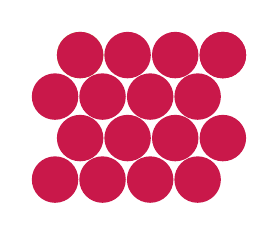
\begin{tikzpicture}[y=1cm, x=1cm,]

				\begin{scope}[shift={(1.3053, -1.5169)}]
					\path[fill=cbada55,draw opacity=0.0] (0.6243, 5.2721).. controls (0.6243, 5.1093) and (0.4921, 4.9771) .. (0.3291, 4.9771).. controls (0.1662, 4.9771) and (0.034, 5.1093) .. (0.034, 5.2721).. controls (0.034, 5.4352) and (0.1662, 5.5673) .. (0.3291, 5.5673).. controls (0.4921, 5.5673) and (0.6243, 5.4352) .. (0.6243, 5.2721) -- cycle(0.6243, 5.2721);

					\path[draw=c2c2c2c,fill=cc9184a,draw opacity=0.0,line width=0.1054cm,miter limit=10.0,cm={ 0.1,-0.0,-0.0,-0.1,(-1.3053, 2.0745)}] (19.2953, -31.9766).. controls (19.2953, -30.3478) and (17.9738, -29.0262) .. (16.3435, -29.0262).. controls (14.7147, -29.0262) and (13.3932, -30.3478) .. (13.3932, -31.9766).. controls (13.3932, -33.6068) and (14.7147, -34.9284) .. (16.3435, -34.9284).. controls (17.9738, -34.9284) and (19.2953, -33.6068) .. (19.2953, -31.9766) -- cycle(19.2953, -31.9766);

				\end{scope}
				\begin{scope}[shift={(1.905, -1.5169)}]
					\path[fill=cc9184a,draw opacity=0.0] (0.6274, 5.2721).. controls (0.6274, 5.1093) and (0.4953, 4.9771) .. (0.3322, 4.9771).. controls (0.1692, 4.9771) and (0.0372, 5.1093) .. (0.0372, 5.2721).. controls (0.0372, 5.4352) and (0.1692, 5.5673) .. (0.3322, 5.5673).. controls (0.4953, 5.5673) and (0.6274, 5.4352) .. (0.6274, 5.2721) -- cycle(0.6274, 5.2721);

					\path[draw=black,draw opacity=0.0,line width=0.1054cm,miter limit=10.0,cm={ 0.1,-0.0,-0.0,-0.1,(-1.905, 2.0745)}] (25.3242, -31.9766).. controls (25.3242, -30.3478) and (24.0027, -29.0262) .. (22.3725, -29.0262).. controls (20.7422, -29.0262) and (19.4221, -30.3478) .. (19.4221, -31.9766).. controls (19.4221, -33.6068) and (20.7422, -34.9284) .. (22.3725, -34.9284).. controls (24.0027, -34.9284) and (25.3242, -33.6068) .. (25.3242, -31.9766) -- cycle(25.3242, -31.9766);

				\end{scope}
				\begin{scope}[shift={(2.54, -1.5169)}]
					\path[fill=cc9184a,draw opacity=0.0] (0.5974, 5.2721).. controls (0.5974, 5.1093) and (0.4652, 4.9771) .. (0.3022, 4.9771).. controls (0.1393, 4.9771) and (0.0072, 5.1093) .. (0.0072, 5.2721).. controls (0.0072, 5.4352) and (0.1393, 5.5673) .. (0.3022, 5.5673).. controls (0.4652, 5.5673) and (0.5974, 5.4352) .. (0.5974, 5.2721) -- cycle(0.5974, 5.2721);

					\path[draw=black,draw opacity=0.0,line width=0.1054cm,miter limit=10.0,cm={ 0.1,-0.0,-0.0,-0.1,(-2.54, 2.0745)}] (31.3738, -31.9766).. controls (31.3738, -30.3478) and (30.0523, -29.0262) .. (28.4221, -29.0262).. controls (26.7932, -29.0262) and (25.4717, -30.3478) .. (25.4717, -31.9766).. controls (25.4717, -33.6068) and (26.7932, -34.9284) .. (28.4221, -34.9284).. controls (30.0523, -34.9284) and (31.3738, -33.6068) .. (31.3738, -31.9766) -- cycle(31.3738, -31.9766);

				\end{scope}
				\begin{scope}[shift={(3.1397, -1.5169)}]
					\path[fill=cc9184a,draw opacity=0.0] (0.6026, 5.2721).. controls (0.6026, 5.1093) and (0.4706, 4.9771) .. (0.3074, 4.9771).. controls (0.1446, 4.9771) and (0.0124, 5.1093) .. (0.0124, 5.2721).. controls (0.0124, 5.4352) and (0.1446, 5.5673) .. (0.3074, 5.5673).. controls (0.4706, 5.5673) and (0.6026, 5.4352) .. (0.6026, 5.2721) -- cycle(0.6026, 5.2721);

					\path[draw=black,fill=cc9184a,draw opacity=0.0,line width=0.1054cm,miter limit=10.0,cm={ 0.1,-0.0,-0.0,-0.1,(-3.1397, 2.0745)}] (37.4234, -31.9766).. controls (37.4234, -30.3478) and (36.1032, -29.0262) .. (34.4716, -29.0262).. controls (32.8428, -29.0262) and (31.5213, -30.3478) .. (31.5213, -31.9766).. controls (31.5213, -33.6068) and (32.8428, -34.9284) .. (34.4716, -34.9284).. controls (36.1032, -34.9284) and (37.4234, -33.6068) .. (37.4234, -31.9766) -- cycle(37.4234, -31.9766);

				\end{scope}
				\begin{scope}[shift={(0.9878, -2.0461)}]
					\path[fill=cc9184a,draw opacity=0.0] (0.6234, 5.2743).. controls (0.6234, 5.1115) and (0.4913, 4.9793) .. (0.3284, 4.9793).. controls (0.1654, 4.9793) and (0.0332, 5.1115) .. (0.0332, 5.2743).. controls (0.0332, 5.4374) and (0.1654, 5.5695) .. (0.3284, 5.5695).. controls (0.4913, 5.5695) and (0.6234, 5.4374) .. (0.6234, 5.2743) -- cycle(0.6234, 5.2743);

					\path[draw=black,draw opacity=0.0,line width=0.1054cm,miter limit=10.0,cm={ 0.1,-0.0,-0.0,-0.1,(-0.9878, 2.6036)}] (16.112, -26.707).. controls (16.112, -25.0781) and (14.7905, -23.7566) .. (13.1617, -23.7566).. controls (11.5314, -23.7566) and (10.2099, -25.0781) .. (10.2099, -26.707).. controls (10.2099, -28.3372) and (11.5314, -29.6587) .. (13.1617, -29.6587).. controls (14.7905, -29.6587) and (16.112, -28.3372) .. (16.112, -26.707) -- cycle(16.112, -26.707);

				\end{scope}
				\begin{scope}[shift={(1.5875, -2.0461)}]
					\path[fill=cc9184a,draw opacity=0.0] (0.6266, 5.2743).. controls (0.6266, 5.1115) and (0.4946, 4.9793) .. (0.3314, 4.9793).. controls (0.1685, 4.9793) and (0.0364, 5.1115) .. (0.0364, 5.2743).. controls (0.0364, 5.4374) and (0.1685, 5.5695) .. (0.3314, 5.5695).. controls (0.4946, 5.5695) and (0.6266, 5.4374) .. (0.6266, 5.2743) -- cycle(0.6266, 5.2743);

					\path[draw=black,draw opacity=0.0,line width=0.1054cm,miter limit=10.0,cm={ 0.1,-0.0,-0.0,-0.1,(-1.5875, 2.6036)}] (22.141, -26.707).. controls (22.141, -25.0781) and (20.8208, -23.7566) .. (19.1892, -23.7566).. controls (17.5604, -23.7566) and (16.2388, -25.0781) .. (16.2388, -26.707).. controls (16.2388, -28.3372) and (17.5604, -29.6587) .. (19.1892, -29.6587).. controls (20.8208, -29.6587) and (22.141, -28.3372) .. (22.141, -26.707) -- cycle(22.141, -26.707);

				\end{scope}
				\begin{scope}[shift={(2.2225, -2.0461)}]
					\path[fill=cc9184a,draw opacity=0.0] (0.5966, 5.2743).. controls (0.5966, 5.1115) and (0.4644, 4.9793) .. (0.3014, 4.9793).. controls (0.1385, 4.9793) and (0.0063, 5.1115) .. (0.0063, 5.2743).. controls (0.0063, 5.4374) and (0.1385, 5.5695) .. (0.3014, 5.5695).. controls (0.4644, 5.5695) and (0.5966, 5.4374) .. (0.5966, 5.2743) -- cycle(0.5966, 5.2743);

					\path[draw=black,draw opacity=0.0,line width=0.1054cm,miter limit=10.0,cm={ 0.1,-0.0,-0.0,-0.1,(-2.2225, 2.6036)}] (28.1905, -26.707).. controls (28.1905, -25.0781) and (26.869, -23.7566) .. (25.2388, -23.7566).. controls (23.6099, -23.7566) and (22.2884, -25.0781) .. (22.2884, -26.707).. controls (22.2884, -28.3372) and (23.6099, -29.6587) .. (25.2388, -29.6587).. controls (26.869, -29.6587) and (28.1905, -28.3372) .. (28.1905, -26.707) -- cycle(28.1905, -26.707);

				\end{scope}
				\begin{scope}[shift={(2.8222, -2.0461)}]
					\path[fill=cc9184a,draw opacity=0.0] (0.5997, 5.2743).. controls (0.5997, 5.1115) and (0.4676, 4.9793) .. (0.3047, 4.9793).. controls (0.1417, 4.9793) and (0.0095, 5.1115) .. (0.0095, 5.2743).. controls (0.0095, 5.4374) and (0.1417, 5.5695) .. (0.3047, 5.5695).. controls (0.4676, 5.5695) and (0.5997, 5.4374) .. (0.5997, 5.2743) -- cycle(0.5997, 5.2743);

					\path[draw=black,draw opacity=0.0,line width=0.1054cm,miter limit=10.0,cm={ 0.1,-0.0,-0.0,-0.1,(-2.8222, 2.6036)}] (34.2195, -26.707).. controls (34.2195, -25.0781) and (32.8979, -23.7566) .. (31.2691, -23.7566).. controls (29.6389, -23.7566) and (28.3173, -25.0781) .. (28.3173, -26.707).. controls (28.3173, -28.3372) and (29.6389, -29.6587) .. (31.2691, -29.6587).. controls (32.8979, -29.6587) and (34.2195, -28.3372) .. (34.2195, -26.707) -- cycle(34.2195, -26.707);

				\end{scope}
				\begin{scope}[shift={(1.3053, -2.54)}]
					\path[fill=cc9184a,draw opacity=0.0] (0.6243, 5.2413).. controls (0.6243, 5.0782) and (0.4921, 4.9461) .. (0.3291, 4.9461).. controls (0.1662, 4.9461) and (0.034, 5.0782) .. (0.034, 5.2413).. controls (0.034, 5.4042) and (0.1662, 5.5363) .. (0.3291, 5.5363).. controls (0.4921, 5.5363) and (0.6243, 5.4042) .. (0.6243, 5.2413) -- cycle(0.6243, 5.2413);

					\path[draw=black,draw opacity=0.0,line width=0.1054cm,miter limit=10.0,cm={ 0.1,-0.0,-0.0,-0.1,(-1.3053, 3.0975)}] (19.2953, -21.4373).. controls (19.2953, -19.8071) and (17.9738, -18.4856) .. (16.3435, -18.4856).. controls (14.7147, -18.4856) and (13.3932, -19.8071) .. (13.3932, -21.4373).. controls (13.3932, -23.0662) and (14.7147, -24.3877) .. (16.3435, -24.3877).. controls (17.9738, -24.3877) and (19.2953, -23.0662) .. (19.2953, -21.4373) -- cycle(19.2953, -21.4373);

				\end{scope}
				\begin{scope}[shift={(1.905, -2.54)}]
					\path[fill=cc9184a,draw opacity=0.0] (0.6274, 5.2413).. controls (0.6274, 5.0782) and (0.4953, 4.9461) .. (0.3322, 4.9461).. controls (0.1692, 4.9461) and (0.0372, 5.0782) .. (0.0372, 5.2413).. controls (0.0372, 5.4042) and (0.1692, 5.5363) .. (0.3322, 5.5363).. controls (0.4953, 5.5363) and (0.6274, 5.4042) .. (0.6274, 5.2413) -- cycle(0.6274, 5.2413);

					\path[draw=black,draw opacity=0.0,line width=0.1054cm,miter limit=10.0,cm={ 0.1,-0.0,-0.0,-0.1,(-1.905, 3.0975)}] (25.3242, -21.4373).. controls (25.3242, -19.8071) and (24.0027, -18.4856) .. (22.3725, -18.4856).. controls (20.7422, -18.4856) and (19.4221, -19.8071) .. (19.4221, -21.4373).. controls (19.4221, -23.0662) and (20.7422, -24.3877) .. (22.3725, -24.3877).. controls (24.0027, -24.3877) and (25.3242, -23.0662) .. (25.3242, -21.4373) -- cycle(25.3242, -21.4373);

				\end{scope}
				\begin{scope}[shift={(2.54, -2.54)}]
					\path[fill=cc9184a,draw opacity=0.0] (0.5974, 5.2413).. controls (0.5974, 5.0782) and (0.4652, 4.9461) .. (0.3022, 4.9461).. controls (0.1393, 4.9461) and (0.0072, 5.0782) .. (0.0072, 5.2413).. controls (0.0072, 5.4042) and (0.1393, 5.5363) .. (0.3022, 5.5363).. controls (0.4652, 5.5363) and (0.5974, 5.4042) .. (0.5974, 5.2413) -- cycle(0.5974, 5.2413);

					\path[draw=black,draw opacity=0.0,line width=0.1054cm,miter limit=10.0,cm={ 0.1,-0.0,-0.0,-0.1,(-2.54, 3.0975)}] (31.3738, -21.4373).. controls (31.3738, -19.8071) and (30.0523, -18.4856) .. (28.4221, -18.4856).. controls (26.7932, -18.4856) and (25.4717, -19.8071) .. (25.4717, -21.4373).. controls (25.4717, -23.0662) and (26.7932, -24.3877) .. (28.4221, -24.3877).. controls (30.0523, -24.3877) and (31.3738, -23.0662) .. (31.3738, -21.4373) -- cycle(31.3738, -21.4373);

				\end{scope}
				\begin{scope}[shift={(3.1397, -2.54)}]
					\path[fill=cc9184a,draw opacity=0.0] (0.6026, 5.2413).. controls (0.6026, 5.0782) and (0.4706, 4.9461) .. (0.3074, 4.9461).. controls (0.1446, 4.9461) and (0.0124, 5.0782) .. (0.0124, 5.2413).. controls (0.0124, 5.4042) and (0.1446, 5.5363) .. (0.3074, 5.5363).. controls (0.4706, 5.5363) and (0.6026, 5.4042) .. (0.6026, 5.2413) -- cycle(0.6026, 5.2413);

					\path[draw=black,draw opacity=0.0,line width=0.1054cm,miter limit=10.0,cm={ 0.1,-0.0,-0.0,-0.1,(-3.1397, 3.0975)}] (37.4234, -21.4373).. controls (37.4234, -19.8071) and (36.1032, -18.4856) .. (34.4716, -18.4856).. controls (32.8428, -18.4856) and (31.5213, -19.8071) .. (31.5213, -21.4373).. controls (31.5213, -23.0662) and (32.8428, -24.3877) .. (34.4716, -24.3877).. controls (36.1032, -24.3877) and (37.4234, -23.0662) .. (37.4234, -21.4373) -- cycle(37.4234, -21.4373);

				\end{scope}
				\begin{scope}[shift={(0.9878, -3.0692)}]
					\path[fill=cc9184a,draw opacity=0.0] (0.6234, 5.2435).. controls (0.6234, 5.0804) and (0.4913, 4.9483) .. (0.3284, 4.9483).. controls (0.1654, 4.9483) and (0.0332, 5.0804) .. (0.0332, 5.2435).. controls (0.0332, 5.4064) and (0.1654, 5.5385) .. (0.3284, 5.5385).. controls (0.4913, 5.5385) and (0.6234, 5.4064) .. (0.6234, 5.2435) -- cycle(0.6234, 5.2435);

					\path[draw=black,draw opacity=0.0,line width=0.1054cm,miter limit=10.0,cm={ 0.1,-0.0,-0.0,-0.1,(-0.9878, 3.6267)}] (16.112, -16.1677).. controls (16.112, -14.5375) and (14.7905, -13.216) .. (13.1617, -13.216).. controls (11.5314, -13.216) and (10.2099, -14.5375) .. (10.2099, -16.1677).. controls (10.2099, -17.7966) and (11.5314, -19.1181) .. (13.1617, -19.1181).. controls (14.7905, -19.1181) and (16.112, -17.7966) .. (16.112, -16.1677) -- cycle(16.112, -16.1677);

				\end{scope}
				\begin{scope}[shift={(1.5875, -3.0692)}]
					\path[fill=cc9184a,draw opacity=0.0] (0.6266, 5.2435).. controls (0.6266, 5.0804) and (0.4946, 4.9483) .. (0.3314, 4.9483).. controls (0.1685, 4.9483) and (0.0364, 5.0804) .. (0.0364, 5.2435).. controls (0.0364, 5.4064) and (0.1685, 5.5385) .. (0.3314, 5.5385).. controls (0.4946, 5.5385) and (0.6266, 5.4064) .. (0.6266, 5.2435) -- cycle(0.6266, 5.2435);

					\path[draw=black,draw opacity=0.0,line width=0.1054cm,miter limit=10.0,cm={ 0.1,-0.0,-0.0,-0.1,(-1.5875, 3.6267)}] (22.141, -16.1677).. controls (22.141, -14.5375) and (20.8208, -13.216) .. (19.1892, -13.216).. controls (17.5604, -13.216) and (16.2388, -14.5375) .. (16.2388, -16.1677).. controls (16.2388, -17.7966) and (17.5604, -19.1181) .. (19.1892, -19.1181).. controls (20.8208, -19.1181) and (22.141, -17.7966) .. (22.141, -16.1677) -- cycle(22.141, -16.1677);

				\end{scope}
				\begin{scope}[shift={(2.2225, -3.0692)}]
					\path[fill=cc9184a,draw opacity=0.0] (0.5966, 5.2435).. controls (0.5966, 5.0804) and (0.4644, 4.9483) .. (0.3014, 4.9483).. controls (0.1385, 4.9483) and (0.0063, 5.0804) .. (0.0063, 5.2435).. controls (0.0063, 5.4064) and (0.1385, 5.5385) .. (0.3014, 5.5385).. controls (0.4644, 5.5385) and (0.5966, 5.4064) .. (0.5966, 5.2435) -- cycle(0.5966, 5.2435);

					\path[draw=black,draw opacity=0.0,line width=0.1054cm,miter limit=10.0,cm={ 0.1,-0.0,-0.0,-0.1,(-2.2225, 3.6267)}] (28.1905, -16.1677).. controls (28.1905, -14.5375) and (26.869, -13.216) .. (25.2388, -13.216).. controls (23.6099, -13.216) and (22.2884, -14.5375) .. (22.2884, -16.1677).. controls (22.2884, -17.7966) and (23.6099, -19.1181) .. (25.2388, -19.1181).. controls (26.869, -19.1181) and (28.1905, -17.7966) .. (28.1905, -16.1677) -- cycle(28.1905, -16.1677);

				\end{scope}
				\begin{scope}[shift={(2.8222, -3.0692)}]
					\path[fill=cc9184a,draw opacity=0.0] (0.5997, 5.2435).. controls (0.5997, 5.0804) and (0.4676, 4.9483) .. (0.3047, 4.9483).. controls (0.1417, 4.9483) and (0.0095, 5.0804) .. (0.0095, 5.2435).. controls (0.0095, 5.4064) and (0.1417, 5.5385) .. (0.3047, 5.5385).. controls (0.4676, 5.5385) and (0.5997, 5.4064) .. (0.5997, 5.2435) -- cycle(0.5997, 5.2435);

					\path[draw=black,draw opacity=0.0,line width=0.1054cm,miter limit=10.0,cm={ 0.1,-0.0,-0.0,-0.1,(-2.8222, 3.6267)}] (34.2195, -16.1677).. controls (34.2195, -14.5375) and (32.8979, -13.216) .. (31.2691, -13.216).. controls (29.6389, -13.216) and (28.3173, -14.5375) .. (28.3173, -16.1677).. controls (28.3173, -17.7966) and (29.6389, -19.1181) .. (31.2691, -19.1181).. controls (32.8979, -19.1181) and (34.2195, -17.7966) .. (34.2195, -16.1677) -- cycle(34.2195, -16.1677);

				\end{scope}
			\end{tikzpicture}
		\end{center}
	\end{minipage}
	\begin{minipage}{5cm}
		\begin{center}
			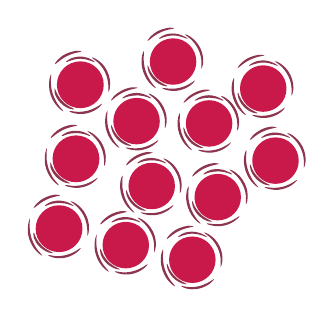
\begin{tikzpicture}[y=1cm, x=1cm]
				\begin{scope}[shift={(5.2211, -1.1642)}]
					\path[draw=black,fill=cc9184a,draw opacity=0.0,line width=0.1054cm,miter limit=10.0,cm={ 0.1,-0.0,-0.0,-0.1,(-5.2211, 1.7217)}] (58.3972, -35.266).. controls (58.3972, -33.6233) and (57.0674, -32.2935) .. (55.4261, -32.2935).. controls (53.7849, -32.2935) and (52.4537, -33.6233) .. (52.4537, -35.266).. controls (52.4537, -36.9072) and (53.7849, -38.237) .. (55.4261, -38.237).. controls (57.0674, -38.237) and (58.3972, -36.9072) .. (58.3972, -35.266) -- cycle(58.3972, -35.266);

				\end{scope}
				\begin{scope}[shift={(5.1153, -1.0231)}]
					\path[fill=c8d354e] (0.4421, 5.5308).. controls (0.4421, 5.5267) and (0.421, 5.5224) .. (0.3872, 5.516).. controls (0.3535, 5.5097) and (0.307, 5.495) .. (0.2629, 5.4739).. controls (0.1701, 5.4296) and (0.1131, 5.3621) .. (0.1047, 5.3707).. controls (0.1027, 5.3727) and (0.1131, 5.3917) .. (0.1364, 5.419).. controls (0.149, 5.4317) and (0.1659, 5.4465) .. (0.1827, 5.4612).. controls (0.2017, 5.4761) and (0.2227, 5.4908) .. (0.2482, 5.5013).. controls (0.2988, 5.5245) and (0.3492, 5.5351) .. (0.383, 5.5393).. controls (0.4188, 5.5393) and (0.4421, 5.5351) .. (0.4421, 5.5308) -- cycle(0.4421, 5.5308);

					\path[fill=c8d354e] (0.0562, 5.2442).. controls (0.0605, 5.2442) and (0.0542, 5.2126) .. (0.0542, 5.1662).. controls (0.0542, 5.1556) and (0.0521, 5.1408) .. (0.0542, 5.1283).. controls (0.0542, 5.1134) and (0.0562, 5.1008) .. (0.0562, 5.0861).. controls (0.0605, 5.0544) and (0.0668, 5.0228) .. (0.0773, 4.9913).. controls (0.09, 4.9575) and (0.1027, 4.928) .. (0.1174, 4.9006).. controls (0.1258, 4.8879) and (0.1322, 4.8753) .. (0.1406, 4.8626).. controls (0.149, 4.8521) and (0.1575, 4.8415) .. (0.1638, 4.831).. controls (0.1933, 4.7952) and (0.2144, 4.7741) .. (0.2122, 4.7719).. controls (0.2102, 4.7678) and (0.1827, 4.7825) .. (0.149, 4.8183).. controls (0.1406, 4.8268) and (0.1301, 4.8352) .. (0.1217, 4.8478).. controls (0.1131, 4.8584) and (0.1027, 4.8732) .. (0.0943, 4.8859).. controls (0.0773, 4.9132) and (0.0605, 4.9449) .. (0.0499, 4.9807).. controls (0.0373, 5.0165) and (0.031, 5.0501) .. (0.031, 5.0839).. controls (0.0288, 5.1008) and (0.0288, 5.1156) .. (0.031, 5.1303).. controls (0.031, 5.1451) and (0.0331, 5.1578) .. (0.0351, 5.1704).. controls (0.0373, 5.1809) and (0.0394, 5.1936) .. (0.0415, 5.202).. controls (0.0435, 5.2126) and (0.0478, 5.2188) .. (0.0499, 5.2251).. controls (0.0499, 5.2378) and (0.0542, 5.2442) .. (0.0562, 5.2442) -- cycle(0.0562, 5.2442);

					\path[fill=c8d354e] (0.2859, 4.7741).. controls (0.2881, 4.7782) and (0.3134, 4.77) .. (0.3514, 4.7678).. controls (0.3914, 4.7614) and (0.4462, 4.7614) .. (0.5053, 4.7741).. controls (0.5643, 4.7867) and (0.6127, 4.812) .. (0.6486, 4.8331).. controls (0.6845, 4.8542) and (0.7014, 4.871) .. (0.7034, 4.8689).. controls (0.7056, 4.8669) and (0.6908, 4.8437) .. (0.6593, 4.8163).. controls (0.6276, 4.7889) and (0.5749, 4.7594) .. (0.5117, 4.7445).. controls (0.4484, 4.7297) and (0.3872, 4.7361) .. (0.3471, 4.7467).. controls (0.307, 4.7551) and (0.284, 4.77) .. (0.2859, 4.7741) -- cycle(0.7856, 5.0165).. controls (0.7813, 5.0165) and (0.7856, 5.0481) .. (0.7836, 5.0945).. controls (0.7813, 5.1408) and (0.7709, 5.2063) .. (0.7414, 5.2673).. controls (0.7119, 5.3306) and (0.6655, 5.3791) .. (0.6317, 5.4065).. controls (0.596, 5.436) and (0.5705, 5.4507) .. (0.5727, 5.455).. controls (0.5749, 5.4571) and (0.6022, 5.4507) .. (0.6444, 5.4233).. controls (0.6634, 5.4106) and (0.6886, 5.3917) .. (0.7097, 5.3685).. controls (0.733, 5.3432) and (0.7519, 5.3158) .. (0.7688, 5.28).. controls (0.8024, 5.2104) and (0.8088, 5.143) .. (0.8046, 5.0945).. controls (0.8024, 5.0439) and (0.7899, 5.0165) .. (0.7856, 5.0165) -- cycle(0.1027, 5.0607).. controls (0.1068, 5.0607) and (0.1131, 5.0397) .. (0.1258, 5.0102).. controls (0.1385, 4.9807) and (0.1638, 4.9385) .. (0.1975, 4.9025).. controls (0.2312, 4.8648) and (0.2734, 4.8394) .. (0.3008, 4.8247).. controls (0.3303, 4.8077) and (0.3514, 4.8015) .. (0.3514, 4.7973).. controls (0.3492, 4.793) and (0.3281, 4.793) .. (0.2923, 4.8036).. controls (0.2587, 4.8141) and (0.2122, 4.8394) .. (0.1743, 4.8795).. controls (0.1342, 4.9195) and (0.1131, 4.9658) .. (0.1027, 5.0018).. controls (0.0984, 5.0376) and (0.1006, 5.0587) .. (0.1027, 5.0607) -- cycle(0.1027, 5.0607);

					\path[fill=c8d354e] (0.6107, 5.3959).. controls (0.6085, 5.3917) and (0.5875, 5.4024) .. (0.5559, 5.4128).. controls (0.5475, 5.4149) and (0.539, 5.419) .. (0.5285, 5.4212).. controls (0.5201, 5.4233) and (0.5095, 5.4276) .. (0.499, 5.4296).. controls (0.4757, 5.4339) and (0.4546, 5.4381) .. (0.4273, 5.4381).. controls (0.402, 5.4381) and (0.3766, 5.436) .. (0.3555, 5.4296).. controls (0.3451, 5.4276) and (0.3345, 5.4254) .. (0.326, 5.4212).. controls (0.3176, 5.419) and (0.307, 5.4149) .. (0.2988, 5.4128).. controls (0.2671, 5.4024) and (0.2482, 5.3917) .. (0.2438, 5.3959).. controls (0.2418, 5.398) and (0.2565, 5.4149) .. (0.2881, 5.4317).. controls (0.2966, 5.436) and (0.305, 5.4401) .. (0.3156, 5.4444).. controls (0.326, 5.4487) and (0.3367, 5.4528) .. (0.3492, 5.455).. controls (0.3725, 5.4612) and (0.3999, 5.4655) .. (0.4251, 5.4655).. controls (0.4525, 5.4655) and (0.48, 5.4612) .. (0.5011, 5.455).. controls (0.5137, 5.4528) and (0.5242, 5.4487) .. (0.5348, 5.4444).. controls (0.5432, 5.4423) and (0.5538, 5.436) .. (0.5622, 5.4317).. controls (0.5979, 5.4149) and (0.6127, 5.4002) .. (0.6107, 5.3959) -- cycle(0.6107, 5.3959);

				\end{scope}
				\begin{scope}[shift={(5.1506, -2.1167)}]
					\path[fill=cc9184a,draw opacity=0.0] (0.6344, 5.2606).. controls (0.6344, 5.0964) and (0.5013, 4.9633) .. (0.3372, 4.9633).. controls (0.1729, 4.9633) and (0.04, 5.0964) .. (0.04, 5.2606).. controls (0.04, 5.4248) and (0.1729, 5.5578) .. (0.3372, 5.5578).. controls (0.5013, 5.5578) and (0.6344, 5.4248) .. (0.6344, 5.2606) -- cycle(0.6344, 5.2606);

					\path[draw=black,draw opacity=0.0,line width=0.1054cm,miter limit=10.0,cm={ 0.1,-0.0,-0.0,-0.1,(-5.1506, 2.6742)}] (57.8501, -25.8636).. controls (57.8501, -24.2224) and (56.5189, -22.8912) .. (54.8777, -22.8912).. controls (53.235, -22.8912) and (51.9052, -24.2224) .. (51.9052, -25.8636).. controls (51.9052, -27.5062) and (53.235, -28.836) .. (54.8777, -28.836).. controls (56.5189, -28.836) and (57.8501, -27.5062) .. (57.8501, -25.8636) -- cycle(57.8501, -25.8636);

				\end{scope}
				\begin{scope}[shift={(5.08, -1.9756)}]
					\path[fill=c8d354e] (0.4225, 5.5432).. controls (0.4225, 5.5389) and (0.4014, 5.5369) .. (0.3678, 5.5285).. controls (0.334, 5.52) and (0.2876, 5.5094) .. (0.2434, 5.4863).. controls (0.1506, 5.442) and (0.0937, 5.3745) .. (0.0852, 5.3829).. controls (0.0831, 5.3851) and (0.0937, 5.4062) .. (0.1169, 5.4314).. controls (0.1295, 5.4462) and (0.1463, 5.4589) .. (0.1632, 5.4736).. controls (0.1822, 5.4883) and (0.2033, 5.501) .. (0.2286, 5.5137).. controls (0.2791, 5.5389) and (0.3298, 5.5494) .. (0.3634, 5.5516).. controls (0.3994, 5.5516) and (0.4225, 5.5475) .. (0.4225, 5.5432) -- cycle(0.4225, 5.5432);

					\path[fill=c8d354e] (0.0367, 5.2566).. controls (0.0409, 5.2544) and (0.0346, 5.2271) .. (0.0346, 5.1786).. controls (0.0346, 5.1659) and (0.0325, 5.1532) .. (0.0346, 5.1405).. controls (0.0346, 5.1258) and (0.0367, 5.1131) .. (0.0367, 5.0963).. controls (0.0409, 5.0668) and (0.0473, 5.033) .. (0.0577, 4.9993).. controls (0.0704, 4.9655) and (0.0831, 4.9362) .. (0.0978, 4.9087).. controls (0.1062, 4.8959) and (0.1126, 4.8834) .. (0.121, 4.8707).. controls (0.1295, 4.8582) and (0.1379, 4.8496) .. (0.1443, 4.8412).. controls (0.1738, 4.8054) and (0.1949, 4.7843) .. (0.1928, 4.7822).. controls (0.1906, 4.778) and (0.1632, 4.7949) .. (0.1295, 4.8285).. controls (0.121, 4.8371) and (0.1105, 4.8455) .. (0.1021, 4.8582).. controls (0.0937, 4.8686) and (0.0831, 4.8834) .. (0.0747, 4.8959).. controls (0.0577, 4.9234) and (0.0409, 4.955) .. (0.0305, 4.9909).. controls (0.0178, 5.0267) and (0.0114, 5.0605) .. (0.0114, 5.0942).. controls (0.0094, 5.111) and (0.0094, 5.1258) .. (0.0114, 5.1405).. controls (0.0114, 5.1553) and (0.0136, 5.168) .. (0.0156, 5.1806).. controls (0.0178, 5.1933) and (0.02, 5.2038) .. (0.0219, 5.2122).. controls (0.0241, 5.2207) and (0.0282, 5.2291) .. (0.0305, 5.2355).. controls (0.0305, 5.2501) and (0.0346, 5.2566) .. (0.0367, 5.2566) -- cycle(0.0367, 5.2566);

					\path[fill=c8d354e] (0.2665, 4.7864).. controls (0.2686, 4.7906) and (0.2939, 4.7822) .. (0.3318, 4.78).. controls (0.3719, 4.7738) and (0.4266, 4.7738) .. (0.4858, 4.7864).. controls (0.5447, 4.7991) and (0.5932, 4.8244) .. (0.6291, 4.8455).. controls (0.6649, 4.8666) and (0.6817, 4.8834) .. (0.6839, 4.8813).. controls (0.686, 4.8793) and (0.6712, 4.856) .. (0.6397, 4.8307).. controls (0.608, 4.8033) and (0.5553, 4.7738) .. (0.4921, 4.759).. controls (0.4288, 4.7442) and (0.3678, 4.7505) .. (0.3276, 4.7612).. controls (0.2876, 4.7675) and (0.2643, 4.7822) .. (0.2665, 4.7864) -- cycle(0.2665, 4.7864);

					\path[fill=c8d354e] (0.7661, 5.0288).. controls (0.7619, 5.031) and (0.7661, 5.0584) .. (0.764, 5.1068).. controls (0.7619, 5.1532) and (0.7513, 5.2185) .. (0.7218, 5.2797).. controls (0.6923, 5.343) and (0.646, 5.3913) .. (0.6123, 5.421).. controls (0.5764, 5.4505) and (0.5511, 5.4652) .. (0.5531, 5.4695).. controls (0.5553, 5.4736) and (0.5828, 5.4652) .. (0.6249, 5.4378).. controls (0.6438, 5.423) and (0.669, 5.404) .. (0.6901, 5.3809).. controls (0.7134, 5.3555) and (0.7323, 5.326) .. (0.7492, 5.2923).. controls (0.783, 5.2227) and (0.7893, 5.1532) .. (0.7851, 5.1068).. controls (0.783, 5.0562) and (0.7703, 5.0288) .. (0.7661, 5.0288) -- cycle(0.7661, 5.0288);

					\path[fill=c8d354e] (0.0831, 5.0731).. controls (0.0874, 5.0752) and (0.0937, 5.0541) .. (0.1062, 5.0224).. controls (0.1189, 4.9929) and (0.1443, 4.9508) .. (0.178, 4.9151).. controls (0.2117, 4.8771) and (0.2538, 4.8539) .. (0.2813, 4.8371).. controls (0.3107, 4.8201) and (0.3318, 4.8138) .. (0.3318, 4.8097).. controls (0.3298, 4.8054) and (0.3087, 4.8054) .. (0.2729, 4.816).. controls (0.2391, 4.8285) and (0.1928, 4.8518) .. (0.1548, 4.8918).. controls (0.1169, 4.9319) and (0.0937, 4.9782) .. (0.0831, 5.014).. controls (0.0788, 5.0499) and (0.081, 5.0709) .. (0.0831, 5.0731) -- cycle(0.5912, 5.4083).. controls (0.5891, 5.404) and (0.568, 5.4146) .. (0.5363, 5.4251).. controls (0.5279, 5.4294) and (0.5195, 5.4314) .. (0.5089, 5.4335).. controls (0.5005, 5.4378) and (0.4899, 5.4398) .. (0.4794, 5.4398).. controls (0.4563, 5.4441) and (0.4352, 5.4462) .. (0.4078, 5.4462).. controls (0.3824, 5.4462) and (0.3572, 5.442) .. (0.3361, 5.4398).. controls (0.3256, 5.4378) and (0.315, 5.4357) .. (0.3065, 5.4335).. controls (0.2982, 5.4314) and (0.2876, 5.4273) .. (0.2791, 5.4251).. controls (0.2475, 5.4124) and (0.2286, 5.404) .. (0.2243, 5.4083).. controls (0.2223, 5.4124) and (0.237, 5.4273) .. (0.2686, 5.4441).. controls (0.2771, 5.4484) and (0.2855, 5.4525) .. (0.296, 5.4568).. controls (0.3065, 5.4609) and (0.3171, 5.4631) .. (0.3298, 5.4673).. controls (0.3529, 5.4736) and (0.3803, 5.4757) .. (0.4056, 5.4757).. controls (0.433, 5.4757) and (0.4604, 5.4715) .. (0.4815, 5.4652).. controls (0.4942, 5.4609) and (0.5048, 5.4589) .. (0.5152, 5.4546).. controls (0.5237, 5.4505) and (0.5343, 5.4462) .. (0.5427, 5.442).. controls (0.5785, 5.4273) and (0.5932, 5.4124) .. (0.5912, 5.4083) -- cycle(0.5912, 5.4083);

				\end{scope}
				\begin{scope}[shift={(4.9389, -2.9986)}]
					\path[fill=cc9184a,draw opacity=0.0] (0.631, 5.255).. controls (0.631, 5.0909) and (0.498, 4.9579) .. (0.3339, 4.9579).. controls (0.1696, 4.9579) and (0.0367, 5.0909) .. (0.0367, 5.255).. controls (0.0367, 5.4193) and (0.1696, 5.5523) .. (0.3339, 5.5523).. controls (0.498, 5.5523) and (0.631, 5.4193) .. (0.631, 5.255) -- cycle(0.631, 5.255);

					\path[draw=black,draw opacity=0.0,line width=0.1054cm,miter limit=10.0,cm={ 0.1,-0.0,-0.0,-0.1,(-4.9389, 3.5561)}] (55.699, -16.989).. controls (55.699, -15.3478) and (54.3692, -14.018) .. (52.7279, -14.018).. controls (51.0853, -14.018) and (49.7555, -15.3478) .. (49.7555, -16.989).. controls (49.7555, -18.6317) and (51.0853, -19.9615) .. (52.7279, -19.9615).. controls (54.3692, -19.9615) and (55.699, -18.6317) .. (55.699, -16.989) -- cycle(55.699, -16.989);

				\end{scope}
				\begin{scope}[shift={(4.8331, -2.8575)}]
					\path[fill=c8d354e] (0.4545, 5.5377).. controls (0.4545, 5.5334) and (0.4334, 5.5313) .. (0.3996, 5.5229).. controls (0.3659, 5.5144) and (0.3196, 5.5039) .. (0.2752, 5.4808).. controls (0.1826, 5.4365) and (0.1255, 5.369) .. (0.1171, 5.3774).. controls (0.1151, 5.3796) and (0.1255, 5.4007) .. (0.1488, 5.4259).. controls (0.1615, 5.4407) and (0.1783, 5.4533) .. (0.1951, 5.4681).. controls (0.2141, 5.4828) and (0.2352, 5.4955) .. (0.2606, 5.5082).. controls (0.311, 5.5334) and (0.3617, 5.544) .. (0.3954, 5.5461).. controls (0.4334, 5.544) and (0.4545, 5.5399) .. (0.4545, 5.5377) -- cycle(0.4545, 5.5377);

					\path[fill=c8d354e] (0.0686, 5.2488).. controls (0.0729, 5.2468) and (0.0666, 5.2194) .. (0.0666, 5.171).. controls (0.0666, 5.1583) and (0.0645, 5.1477) .. (0.0666, 5.133).. controls (0.0666, 5.1203) and (0.0686, 5.1033) .. (0.0686, 5.0887).. controls (0.0729, 5.0592) and (0.0792, 5.0255) .. (0.0897, 4.9917).. controls (0.1024, 4.9579) and (0.1151, 4.9285) .. (0.1298, 4.901).. controls (0.1382, 4.8884) and (0.1446, 4.8758) .. (0.153, 4.8631).. controls (0.1615, 4.8505) and (0.1699, 4.842) .. (0.1763, 4.8336).. controls (0.2056, 4.7977) and (0.2268, 4.7788) .. (0.2248, 4.7725).. controls (0.2226, 4.7704) and (0.1951, 4.7851) .. (0.1615, 4.8188).. controls (0.153, 4.8273) and (0.1425, 4.8379) .. (0.1341, 4.8484).. controls (0.1255, 4.859) and (0.1151, 4.8715) .. (0.1067, 4.8864).. controls (0.0897, 4.9137) and (0.0729, 4.9453) .. (0.0623, 4.9812).. controls (0.0497, 5.0171) and (0.0434, 5.0529) .. (0.0434, 5.0844).. controls (0.0412, 5.1014) and (0.0412, 5.1161) .. (0.0434, 5.1288).. controls (0.0434, 5.1436) and (0.0455, 5.1561) .. (0.0475, 5.1688).. controls (0.0497, 5.1793) and (0.0518, 5.1921) .. (0.0539, 5.2003).. controls (0.0561, 5.2087) and (0.0602, 5.2173) .. (0.0623, 5.2236).. controls (0.0645, 5.2425) and (0.0666, 5.2488) .. (0.0686, 5.2488) -- cycle(0.0686, 5.2488);

					\path[fill=c8d354e] (0.2985, 4.7788).. controls (0.3006, 4.7831) and (0.3258, 4.7766) .. (0.3638, 4.7704).. controls (0.4039, 4.7641) and (0.4586, 4.762) .. (0.5177, 4.7766).. controls (0.5767, 4.7894) and (0.6252, 4.8146) .. (0.661, 4.8357).. controls (0.6969, 4.8568) and (0.7137, 4.8736) .. (0.7158, 4.8695).. controls (0.718, 4.8673) and (0.7032, 4.8462) .. (0.6715, 4.8188).. controls (0.64, 4.7915) and (0.5872, 4.762) .. (0.5241, 4.7472).. controls (0.4608, 4.7325) and (0.3996, 4.7388) .. (0.3595, 4.7493).. controls (0.3196, 4.762) and (0.2985, 4.7766) .. (0.2985, 4.7788) -- cycle(0.2985, 4.7788);

					\path[fill=c8d354e] (0.8001, 5.0234).. controls (0.796, 5.0255) and (0.8001, 5.0529) .. (0.798, 5.0992).. controls (0.796, 5.1455) and (0.7853, 5.211) .. (0.7559, 5.272).. controls (0.7264, 5.3352) and (0.6799, 5.3838) .. (0.6463, 5.4134).. controls (0.6103, 5.4429) and (0.5851, 5.4576) .. (0.5872, 5.4618).. controls (0.5892, 5.466) and (0.6167, 5.4576) .. (0.6588, 5.4301).. controls (0.6779, 5.4155) and (0.7032, 5.3964) .. (0.7243, 5.3733).. controls (0.7474, 5.3479) and (0.7665, 5.3184) .. (0.7833, 5.2847).. controls (0.817, 5.2151) and (0.8234, 5.1477) .. (0.8191, 5.0992).. controls (0.815, 5.0507) and (0.8023, 5.0212) .. (0.8001, 5.0234) -- cycle(0.8001, 5.0234);

					\path[fill=c8d354e] (0.1171, 5.0656).. controls (0.1214, 5.0676) and (0.1277, 5.0466) .. (0.1404, 5.0149).. controls (0.153, 4.9833) and (0.1783, 4.9432) .. (0.2121, 4.9075).. controls (0.2458, 4.8695) and (0.2879, 4.8462) .. (0.3153, 4.8316).. controls (0.3448, 4.8146) and (0.3659, 4.8083) .. (0.3659, 4.8042).. controls (0.3638, 4.8021) and (0.3427, 4.7999) .. (0.3069, 4.8126).. controls (0.2731, 4.8251) and (0.2268, 4.8484) .. (0.1888, 4.8884).. controls (0.1488, 4.9285) and (0.1277, 4.9749) .. (0.1171, 5.0107).. controls (0.113, 5.0423) and (0.113, 5.0656) .. (0.1171, 5.0656) -- cycle(0.6252, 5.4028).. controls (0.623, 5.3985) and (0.6019, 5.4091) .. (0.5704, 5.4196).. controls (0.562, 5.4239) and (0.5534, 5.4259) .. (0.5429, 5.4281).. controls (0.5345, 5.4323) and (0.5241, 5.4345) .. (0.5135, 5.4345).. controls (0.4903, 5.4386) and (0.4692, 5.4407) .. (0.4418, 5.4407).. controls (0.4164, 5.4407) and (0.3912, 5.4365) .. (0.3701, 5.4345).. controls (0.3595, 5.4323) and (0.3491, 5.4301) .. (0.3407, 5.4281).. controls (0.3321, 5.4259) and (0.3216, 5.4218) .. (0.3132, 5.4196).. controls (0.2815, 5.407) and (0.2625, 5.3985) .. (0.2584, 5.4028).. controls (0.2563, 5.407) and (0.2711, 5.4218) .. (0.3026, 5.4386).. controls (0.311, 5.4429) and (0.3196, 5.447) .. (0.33, 5.4511).. controls (0.3407, 5.4556) and (0.3511, 5.4576) .. (0.3638, 5.4618).. controls (0.387, 5.4681) and (0.4144, 5.4703) .. (0.4397, 5.4703).. controls (0.4672, 5.4703) and (0.4944, 5.466) .. (0.5155, 5.4597).. controls (0.5282, 5.4556) and (0.5387, 5.4533) .. (0.5493, 5.4492).. controls (0.5577, 5.4449) and (0.5682, 5.4407) .. (0.5767, 5.4365).. controls (0.6103, 5.4218) and (0.6273, 5.4048) .. (0.6252, 5.4028) -- cycle(0.6252, 5.4028);

				\end{scope}
				\begin{scope}[shift={(5.7856, -3.2103)}]
					\path[fill=cc9184a,draw opacity=0.0] (0.6296, 5.2581).. controls (0.6296, 5.0951) and (0.4975, 4.9629) .. (0.3346, 4.9629).. controls (0.1716, 4.9629) and (0.0394, 5.0951) .. (0.0394, 5.2581).. controls (0.0394, 5.421) and (0.1716, 5.5531) .. (0.3346, 5.5531).. controls (0.4975, 5.5531) and (0.6296, 5.421) .. (0.6296, 5.2581) -- cycle(0.6296, 5.2581);

					\path[draw=black,draw opacity=0.0,line width=0.1054cm,miter limit=10.0,cm={ 0.1,-0.0,-0.0,-0.1,(-5.7856, 3.7678)}] (64.1519, -14.9027).. controls (64.1519, -13.2725) and (62.8303, -11.9509) .. (61.2015, -11.9509).. controls (59.5713, -11.9509) and (58.2497, -13.2725) .. (58.2497, -14.9027).. controls (58.2497, -16.5315) and (59.5713, -17.8531) .. (61.2015, -17.8531).. controls (62.8303, -17.8531) and (64.1519, -16.5315) .. (64.1519, -14.9027) -- cycle(64.1519, -14.9027);

				\end{scope}
				\begin{scope}[shift={(5.715, -3.0692)}]
					\path[fill=c8d354e] (0.4199, 5.5407).. controls (0.4199, 5.5364) and (0.3988, 5.5344) .. (0.3652, 5.5258).. controls (0.3314, 5.5174) and (0.285, 5.507) .. (0.2387, 5.4837).. controls (0.1458, 5.4394) and (0.0889, 5.372) .. (0.0805, 5.3804).. controls (0.0784, 5.3827) and (0.0889, 5.4037) .. (0.1122, 5.429).. controls (0.1247, 5.4437) and (0.1417, 5.4564) .. (0.1585, 5.4711).. controls (0.1775, 5.4859) and (0.1986, 5.4985) .. (0.2238, 5.5111).. controls (0.2723, 5.5364) and (0.323, 5.5469) .. (0.3588, 5.5491).. controls (0.3988, 5.5491) and (0.4199, 5.5448) .. (0.4199, 5.5407) -- cycle(0.4199, 5.5407);

					\path[fill=c8d354e] (0.034, 5.2539).. controls (0.0384, 5.2519) and (0.032, 5.2245) .. (0.032, 5.178).. controls (0.032, 5.1655) and (0.0299, 5.1549) .. (0.032, 5.1401).. controls (0.032, 5.1274) and (0.034, 5.1106) .. (0.034, 5.0959).. controls (0.0384, 5.0664) and (0.0446, 5.0326) .. (0.0551, 4.9989).. controls (0.0678, 4.9652) and (0.0805, 4.9356) .. (0.0952, 4.9083).. controls (0.1036, 4.8957) and (0.11, 4.883) .. (0.1184, 4.8703).. controls (0.1269, 4.8576) and (0.1353, 4.8492) .. (0.1417, 4.8408).. controls (0.1712, 4.805) and (0.1922, 4.786) .. (0.1902, 4.7796).. controls (0.188, 4.7776) and (0.1605, 4.7924) .. (0.1269, 4.8261).. controls (0.1184, 4.8345) and (0.1079, 4.8451) .. (0.0995, 4.8556).. controls (0.0911, 4.8662) and (0.0805, 4.8787) .. (0.0721, 4.8934).. controls (0.0551, 4.9209) and (0.0384, 4.9526) .. (0.0278, 4.9883).. controls (0.0152, 5.0242) and (0.0088, 5.0601) .. (0.0088, 5.0917).. controls (0.0068, 5.1086) and (0.0068, 5.1233) .. (0.0088, 5.1358).. controls (0.0088, 5.1507) and (0.011, 5.1633) .. (0.013, 5.1759).. controls (0.0152, 5.1886) and (0.0174, 5.1991) .. (0.0193, 5.2076).. controls (0.0215, 5.216) and (0.0258, 5.2245) .. (0.0278, 5.2308).. controls (0.0299, 5.2476) and (0.032, 5.2539) .. (0.034, 5.2539) -- cycle(0.034, 5.2539);

					\path[fill=c8d354e] (0.2639, 4.7839).. controls (0.2639, 4.788) and (0.2913, 4.7818) .. (0.3292, 4.7755).. controls (0.3693, 4.7692) and (0.424, 4.7669) .. (0.4831, 4.7818).. controls (0.5421, 4.7944) and (0.5906, 4.8197) .. (0.6265, 4.8408).. controls (0.6623, 4.8619) and (0.6792, 4.8787) .. (0.6813, 4.8746).. controls (0.6834, 4.8724) and (0.6708, 4.8513) .. (0.6371, 4.824).. controls (0.6054, 4.7966) and (0.5527, 4.7669) .. (0.4895, 4.7522).. controls (0.4262, 4.7375) and (0.3652, 4.7439) .. (0.3251, 4.7544).. controls (0.285, 4.765) and (0.2639, 4.7796) .. (0.2639, 4.7839) -- cycle(0.2639, 4.7839);

					\path[fill=c8d354e] (0.7656, 5.0263).. controls (0.7614, 5.0285) and (0.7656, 5.0559) .. (0.7656, 5.1022).. controls (0.7656, 5.1485) and (0.755, 5.214) .. (0.7235, 5.275).. controls (0.6918, 5.3383) and (0.6496, 5.3868) .. (0.6138, 5.4163).. controls (0.5779, 5.4459) and (0.5527, 5.4605) .. (0.5548, 5.4648).. controls (0.5548, 5.4689) and (0.5865, 5.4605) .. (0.6265, 5.4331).. controls (0.6475, 5.4183) and (0.6686, 5.3993) .. (0.6918, 5.3763).. controls (0.713, 5.353) and (0.7341, 5.3215) .. (0.7508, 5.2898).. controls (0.7845, 5.2202) and (0.7909, 5.1507) .. (0.7867, 5.1022).. controls (0.7804, 5.0537) and (0.7677, 5.0263) .. (0.7656, 5.0263) -- cycle(0.7656, 5.0263);

					\path[fill=c8d354e] (0.0825, 5.0707).. controls (0.0868, 5.0726) and (0.0932, 5.0515) .. (0.1058, 5.02).. controls (0.1184, 4.9883) and (0.1437, 4.9483) .. (0.1775, 4.9125).. controls (0.2113, 4.8746) and (0.2534, 4.8513) .. (0.2808, 4.8365).. controls (0.3103, 4.8197) and (0.3314, 4.8134) .. (0.3314, 4.8091).. controls (0.3314, 4.807) and (0.3081, 4.805) .. (0.2723, 4.8177).. controls (0.2387, 4.8302) and (0.1922, 4.8535) .. (0.1543, 4.8934).. controls (0.1142, 4.9336) and (0.0932, 4.98) .. (0.0825, 5.0158).. controls (0.0784, 5.0474) and (0.0784, 5.0685) .. (0.0825, 5.0707) -- cycle(0.5906, 5.4057).. controls (0.5886, 5.4015) and (0.5695, 5.412) .. (0.538, 5.4226).. controls (0.5294, 5.4268) and (0.521, 5.429) .. (0.5106, 5.431).. controls (0.5, 5.4353) and (0.4895, 5.4374) .. (0.4789, 5.4374).. controls (0.4578, 5.4415) and (0.4346, 5.4437) .. (0.4073, 5.4437).. controls (0.3819, 5.4437) and (0.3566, 5.4394) .. (0.3356, 5.4374).. controls (0.3251, 5.4353) and (0.3145, 5.4331) .. (0.3039, 5.431).. controls (0.2934, 5.429) and (0.285, 5.4248) .. (0.2766, 5.4226).. controls (0.2449, 5.4099) and (0.226, 5.4015) .. (0.2217, 5.4057).. controls (0.2197, 5.4099) and (0.2365, 5.4248) .. (0.2682, 5.4415).. controls (0.2766, 5.4459) and (0.285, 5.45) .. (0.2956, 5.4542).. controls (0.3061, 5.4584) and (0.3167, 5.4605) .. (0.3271, 5.4648).. controls (0.3503, 5.4711) and (0.3777, 5.4732) .. (0.4029, 5.4732).. controls (0.4284, 5.4732) and (0.4557, 5.4689) .. (0.4789, 5.4626).. controls (0.4895, 5.4584) and (0.5, 5.4564) .. (0.5106, 5.4521).. controls (0.521, 5.4478) and (0.5294, 5.4437) .. (0.538, 5.4394).. controls (0.5759, 5.4248) and (0.5927, 5.4099) .. (0.5906, 5.4057) -- cycle(0.5906, 5.4057);

				\end{scope}
				\begin{scope}[shift={(6.6322, -3.3867)}]
					\path[fill=cc9184a,draw opacity=0.0] (0.6284, 5.249).. controls (0.6284, 5.086) and (0.4962, 4.9538) .. (0.3332, 4.9538).. controls (0.1702, 4.9538) and (0.038, 5.086) .. (0.038, 5.249).. controls (0.038, 5.412) and (0.1702, 5.544) .. (0.3332, 5.544).. controls (0.4962, 5.544) and (0.6284, 5.412) .. (0.6284, 5.249) -- cycle(0.6284, 5.249);

					\path[draw=black,draw opacity=0.0,line width=0.1054cm,miter limit=10.0,cm={ 0.1,-0.0,-0.0,-0.1,(-6.6322, 3.9442)}] (72.6061, -13.0478).. controls (72.6061, -11.4176) and (71.2846, -10.0961) .. (69.6544, -10.0961).. controls (68.0241, -10.0961) and (66.7026, -11.4176) .. (66.7026, -13.0478).. controls (66.7026, -14.6781) and (68.0241, -15.9982) .. (69.6544, -15.9982).. controls (71.2846, -15.9982) and (72.6061, -14.6781) .. (72.6061, -13.0478) -- cycle(72.6061, -13.0478);

				\end{scope}
				\begin{scope}[shift={(6.5617, -3.2456)}]
					\path[fill=c8d354e] (0.4185, 5.5316).. controls (0.4185, 5.5273) and (0.3974, 5.5231) .. (0.3637, 5.5169).. controls (0.33, 5.5083) and (0.2836, 5.4979) .. (0.2372, 5.4747).. controls (0.1424, 5.4303) and (0.0876, 5.3629) .. (0.0791, 5.3714).. controls (0.077, 5.3734) and (0.0876, 5.3945) .. (0.1108, 5.4199).. controls (0.1213, 5.4325) and (0.1403, 5.4473) .. (0.1571, 5.462).. controls (0.1761, 5.4768) and (0.1993, 5.4914) .. (0.2224, 5.502).. controls (0.273, 5.5253) and (0.3237, 5.5358) .. (0.3573, 5.5399).. controls (0.3974, 5.538) and (0.4185, 5.5335) .. (0.4185, 5.5316) -- cycle(0.4185, 5.5316);

					\path[fill=c8d354e] (0.0328, 5.2428).. controls (0.0369, 5.2406) and (0.0328, 5.2132) .. (0.0306, 5.1669).. controls (0.0306, 5.1542) and (0.0306, 5.1437) .. (0.0306, 5.129).. controls (0.0306, 5.1163) and (0.0306, 5.0995) .. (0.0328, 5.0847).. controls (0.0369, 5.0551) and (0.0433, 5.0215) .. (0.0539, 4.9877).. controls (0.0644, 4.9539) and (0.0791, 4.9245) .. (0.0938, 4.897).. controls (0.1024, 4.8845) and (0.1086, 4.8718) .. (0.117, 4.859).. controls (0.1254, 4.8465) and (0.1339, 4.8381) .. (0.1381, 4.8296).. controls (0.1676, 4.7938) and (0.1887, 4.7748) .. (0.1866, 4.7685).. controls (0.1845, 4.7664) and (0.1571, 4.7811) .. (0.1233, 4.8149).. controls (0.1149, 4.8233) and (0.1045, 4.8338) .. (0.096, 4.8444).. controls (0.0854, 4.8549) and (0.077, 4.8675) .. (0.0685, 4.8823).. controls (0.0517, 4.9097) and (0.0369, 4.9414) .. (0.0244, 4.9771).. controls (0.0138, 5.0129) and (0.0054, 5.0488) .. (0.0033, 5.0804).. controls (0.0033, 5.0973) and (0.0033, 5.112) .. (0.0033, 5.1247).. controls (0.0033, 5.1394) and (0.0054, 5.1521) .. (0.0074, 5.1646).. controls (0.0074, 5.1775) and (0.0117, 5.1879) .. (0.0138, 5.1963).. controls (0.0158, 5.2049) and (0.0201, 5.2132) .. (0.0222, 5.2196).. controls (0.0285, 5.2364) and (0.0306, 5.2428) .. (0.0328, 5.2428) -- cycle(0.0328, 5.2428);

					\path[fill=c8d354e] (0.2625, 4.7727).. controls (0.2625, 4.7769) and (0.2899, 4.7705) .. (0.3278, 4.7642).. controls (0.3679, 4.758) and (0.4228, 4.7558) .. (0.4818, 4.7705).. controls (0.5407, 4.7832) and (0.5892, 4.8086) .. (0.6251, 4.8296).. controls (0.6609, 4.8507) and (0.6779, 4.8675) .. (0.6799, 4.8634).. controls (0.682, 4.8612) and (0.6693, 4.8401) .. (0.6357, 4.8127).. controls (0.604, 4.7853) and (0.5514, 4.7558) .. (0.4881, 4.741).. controls (0.4248, 4.7263) and (0.3637, 4.7326) .. (0.3237, 4.7431).. controls (0.2836, 4.7558) and (0.2625, 4.7705) .. (0.2625, 4.7727) -- cycle(0.2625, 4.7727);

					\path[fill=c8d354e] (0.7641, 5.0172).. controls (0.76, 5.0193) and (0.7641, 5.0467) .. (0.7641, 5.0931).. controls (0.7641, 5.1394) and (0.7536, 5.2049) .. (0.7221, 5.2659).. controls (0.6904, 5.3292) and (0.6482, 5.3777) .. (0.6124, 5.4051).. controls (0.5766, 5.4346) and (0.5514, 5.4494) .. (0.5534, 5.4536).. controls (0.5534, 5.4557) and (0.585, 5.4494) .. (0.6251, 5.4219).. controls (0.6462, 5.4093) and (0.6672, 5.3882) .. (0.6904, 5.3671).. controls (0.7115, 5.3439) and (0.7326, 5.3122) .. (0.7495, 5.2807).. controls (0.7833, 5.2112) and (0.7895, 5.1416) .. (0.7853, 5.0931).. controls (0.7789, 5.0446) and (0.7663, 5.0151) .. (0.7641, 5.0172) -- cycle(0.7641, 5.0172);

					\path[fill=c8d354e] (0.0813, 5.0594).. controls (0.0854, 5.0614) and (0.0918, 5.0403) .. (0.1045, 5.0088).. controls (0.117, 4.9771) and (0.1424, 4.9371) .. (0.1782, 4.9012).. controls (0.2119, 4.8634) and (0.2519, 4.8401) .. (0.2836, 4.8254).. controls (0.3131, 4.8086) and (0.3342, 4.8022) .. (0.3342, 4.798).. controls (0.3342, 4.7959) and (0.311, 4.7938) .. (0.2752, 4.8064).. controls (0.2414, 4.819) and (0.195, 4.8423) .. (0.1571, 4.8823).. controls (0.117, 4.9223) and (0.096, 4.9688) .. (0.0854, 5.0045).. controls (0.077, 5.0362) and (0.077, 5.0594) .. (0.0813, 5.0594) -- cycle(0.5892, 5.3966).. controls (0.5872, 5.3924) and (0.5682, 5.4029) .. (0.5365, 5.4135).. controls (0.5281, 5.4156) and (0.5197, 5.4199) .. (0.5092, 5.4219).. controls (0.4987, 5.424) and (0.4881, 5.4283) .. (0.4776, 5.4303).. controls (0.4565, 5.4346) and (0.4333, 5.4387) .. (0.4058, 5.4387).. controls (0.3806, 5.4387) and (0.3553, 5.4367) .. (0.3342, 5.4303).. controls (0.3237, 5.4283) and (0.3131, 5.4262) .. (0.3026, 5.4219).. controls (0.292, 5.4199) and (0.2836, 5.4156) .. (0.2752, 5.4135).. controls (0.2435, 5.4008) and (0.2224, 5.3924) .. (0.2224, 5.3966).. controls (0.2203, 5.3988) and (0.2351, 5.4156) .. (0.2668, 5.4325).. controls (0.2752, 5.4367) and (0.2836, 5.4409) .. (0.2941, 5.4451).. controls (0.3047, 5.4494) and (0.3152, 5.4536) .. (0.3258, 5.4557).. controls (0.3489, 5.462) and (0.3763, 5.4641) .. (0.4017, 5.4641).. controls (0.4269, 5.4641) and (0.4543, 5.4598) .. (0.4776, 5.4536).. controls (0.4881, 5.4514) and (0.4987, 5.4473) .. (0.5092, 5.443).. controls (0.5197, 5.4409) and (0.5281, 5.4346) .. (0.5365, 5.4303).. controls (0.5745, 5.4156) and (0.5913, 5.3988) .. (0.5892, 5.3966) -- cycle(0.5892, 5.3966);

				\end{scope}
				\begin{scope}[shift={(6.1383, -2.4694)}]
					\path[draw=black,fill=cc9184a,draw opacity=0.0,line width=0.1054cm,miter limit=10.0,cm={ 0.1,-0.0,-0.0,-0.1,(-6.1383, 3.027)}] (67.4412, -22.4075).. controls (67.4412, -20.7773) and (66.1197, -19.4557) .. (64.4909, -19.4557).. controls (62.8593, -19.4557) and (61.5391, -20.7773) .. (61.5391, -22.4075).. controls (61.5391, -24.0363) and (62.8593, -25.3579) .. (64.4909, -25.3579).. controls (66.1197, -25.3579) and (67.4412, -24.0363) .. (67.4412, -22.4075) -- cycle(67.4412, -22.4075);

				\end{scope}
				\begin{scope}[shift={(6.0325, -2.2931)}]
					\path[fill=c8d354e] (0.4312, 5.5149).. controls (0.4312, 5.5108) and (0.4102, 5.5086) .. (0.3765, 5.5002).. controls (0.3427, 5.4918) and (0.2963, 5.4813) .. (0.25, 5.458).. controls (0.155, 5.4138) and (0.1003, 5.3463) .. (0.0918, 5.3548).. controls (0.0898, 5.3569) and (0.1003, 5.378) .. (0.1235, 5.4032).. controls (0.1339, 5.4181) and (0.1531, 5.4306) .. (0.1698, 5.4454).. controls (0.1888, 5.4602) and (0.2119, 5.4728) .. (0.2352, 5.4855).. controls (0.2858, 5.5108) and (0.3364, 5.5213) .. (0.37, 5.5235).. controls (0.408, 5.5213) and (0.4312, 5.5172) .. (0.4312, 5.5149) -- cycle(0.4312, 5.5149);

					\path[fill=c8d354e] (0.0455, 5.2262).. controls (0.0496, 5.224) and (0.0455, 5.1968) .. (0.0433, 5.1482).. controls (0.0433, 5.1356) and (0.0433, 5.1229) .. (0.0433, 5.1102).. controls (0.0433, 5.0955) and (0.0433, 5.0828) .. (0.0455, 5.066).. controls (0.0496, 5.0365) and (0.0561, 5.0027) .. (0.0666, 4.969).. controls (0.077, 4.9352) and (0.0918, 4.9059) .. (0.1065, 4.8784).. controls (0.1151, 4.8656) and (0.1214, 4.8531) .. (0.1298, 4.8404).. controls (0.1382, 4.8279) and (0.1466, 4.8193) .. (0.1509, 4.8109).. controls (0.1804, 4.7751) and (0.2015, 4.754) .. (0.1994, 4.7519).. controls (0.1972, 4.7477) and (0.1698, 4.7646) .. (0.1362, 4.7982).. controls (0.1276, 4.8068) and (0.1171, 4.8152) .. (0.1087, 4.8279).. controls (0.0981, 4.8383) and (0.0898, 4.8531) .. (0.0813, 4.8656).. controls (0.0644, 4.8932) and (0.0496, 4.9247) .. (0.0371, 4.9606).. controls (0.0266, 4.9965) and (0.0181, 5.0302) .. (0.016, 5.0639).. controls (0.016, 5.0807) and (0.016, 5.0955) .. (0.016, 5.1102).. controls (0.016, 5.125) and (0.0181, 5.1376) .. (0.0201, 5.1503).. controls (0.0201, 5.163) and (0.0244, 5.1735) .. (0.0266, 5.1819).. controls (0.0285, 5.1904) and (0.0328, 5.1988) .. (0.0349, 5.2052).. controls (0.0391, 5.2199) and (0.0433, 5.2262) .. (0.0455, 5.2262) -- cycle(0.0455, 5.2262);

					\path[fill=c8d354e] (0.2752, 4.7561).. controls (0.2752, 4.7603) and (0.3026, 4.7519) .. (0.3405, 4.7497).. controls (0.3806, 4.7435) and (0.4355, 4.7435) .. (0.4944, 4.7561).. controls (0.5536, 4.7687) and (0.6019, 4.7941) .. (0.6378, 4.8152).. controls (0.6737, 4.8363) and (0.6905, 4.8531) .. (0.6926, 4.851).. controls (0.6947, 4.8489) and (0.6821, 4.8257) .. (0.6484, 4.8004).. controls (0.6168, 4.773) and (0.564, 4.7435) .. (0.5008, 4.7286).. controls (0.4375, 4.7139) and (0.3765, 4.7202) .. (0.3364, 4.7308).. controls (0.2963, 4.7392) and (0.2731, 4.754) .. (0.2752, 4.7561) -- cycle(0.2752, 4.7561);

					\path[fill=c8d354e] (0.7749, 5.0007).. controls (0.7706, 5.0027) and (0.7749, 5.0302) .. (0.7749, 5.0787).. controls (0.7749, 5.125) and (0.7643, 5.1904) .. (0.7327, 5.2515).. controls (0.701, 5.3147) and (0.659, 5.3632) .. (0.623, 5.3927).. controls (0.5872, 5.4222) and (0.562, 5.4369) .. (0.564, 5.4412).. controls (0.564, 5.4454) and (0.5957, 5.4369) .. (0.6357, 5.4095).. controls (0.6568, 5.3948) and (0.6779, 5.3759) .. (0.701, 5.3526).. controls (0.7222, 5.3274) and (0.7432, 5.2978) .. (0.76, 5.2641).. controls (0.7938, 5.1946) and (0.8001, 5.125) .. (0.796, 5.0787).. controls (0.7917, 5.0281) and (0.7791, 4.9985) .. (0.7749, 5.0007) -- cycle(0.7749, 5.0007);

					\path[fill=c8d354e] (0.0918, 5.0428).. controls (0.096, 5.0449) and (0.1024, 5.0238) .. (0.1151, 4.9921).. controls (0.1276, 4.9626) and (0.1531, 4.9206) .. (0.1888, 4.8848).. controls (0.2226, 4.8467) and (0.2627, 4.8236) .. (0.2942, 4.8068).. controls (0.3237, 4.7898) and (0.3448, 4.7835) .. (0.3448, 4.7793).. controls (0.3448, 4.7751) and (0.3216, 4.7751) .. (0.2858, 4.7857).. controls (0.252, 4.7982) and (0.2057, 4.8215) .. (0.1677, 4.8615).. controls (0.1298, 4.9016) and (0.1065, 4.948) .. (0.096, 4.9837).. controls (0.0876, 5.0195) and (0.0898, 5.0428) .. (0.0918, 5.0428) -- cycle(0.5999, 5.38).. controls (0.5977, 5.3759) and (0.5788, 5.3864) .. (0.5472, 5.397).. controls (0.5387, 5.4011) and (0.5303, 5.4032) .. (0.5198, 5.4054).. controls (0.5092, 5.4095) and (0.4987, 5.4117) .. (0.4881, 5.4117).. controls (0.467, 5.4159) and (0.4439, 5.4181) .. (0.4166, 5.4181).. controls (0.3911, 5.4181) and (0.3659, 5.4138) .. (0.3448, 5.4117).. controls (0.3343, 5.4095) and (0.3237, 5.4075) .. (0.3132, 5.4054).. controls (0.3026, 5.4032) and (0.2942, 5.3991) .. (0.2858, 5.397).. controls (0.2541, 5.3843) and (0.233, 5.3759) .. (0.233, 5.38).. controls (0.231, 5.3843) and (0.2457, 5.3991) .. (0.2774, 5.4159).. controls (0.2858, 5.4201) and (0.2942, 5.4243) .. (0.3048, 5.4285).. controls (0.3153, 5.4328) and (0.3259, 5.4349) .. (0.3364, 5.4392).. controls (0.3595, 5.4454) and (0.387, 5.4476) .. (0.4122, 5.4476).. controls (0.4375, 5.4476) and (0.465, 5.4433) .. (0.4881, 5.4369).. controls (0.4987, 5.4328) and (0.5092, 5.4306) .. (0.5198, 5.4265).. controls (0.5303, 5.4222) and (0.5387, 5.4181) .. (0.5472, 5.4138).. controls (0.5872, 5.3991) and (0.6019, 5.3821) .. (0.5999, 5.38) -- cycle(0.5999, 5.38);

				\end{scope}
				\begin{scope}[shift={(6.8439, -1.6581)}]
					\path[fill=cc9184a,draw opacity=0.0] (0.6295, 5.2511).. controls (0.6295, 5.0879) and (0.4975, 4.9559) .. (0.3345, 4.9559).. controls (0.1714, 4.9559) and (0.0393, 5.0879) .. (0.0393, 5.2511).. controls (0.0393, 5.4139) and (0.1714, 5.5461) .. (0.3345, 5.5461).. controls (0.4975, 5.5461) and (0.6295, 5.4139) .. (0.6295, 5.2511) -- cycle(0.6295, 5.2511);

					\path[draw=black,draw opacity=0.0,line width=0.1054cm,miter limit=10.0,cm={ 0.1,-0.0,-0.0,-0.1,(-6.8439, 2.2156)}] (74.7338, -30.3546).. controls (74.7338, -28.723) and (73.4137, -27.4029) .. (71.7834, -27.4029).. controls (70.1532, -27.4029) and (68.8317, -28.723) .. (68.8317, -30.3546).. controls (68.8317, -31.9835) and (70.1532, -33.305) .. (71.7834, -33.305).. controls (73.4137, -33.305) and (74.7338, -31.9835) .. (74.7338, -30.3546) -- cycle(74.7338, -30.3546);

				\end{scope}
				\begin{scope}[shift={(6.7733, -1.5169)}]
					\path[fill=c8d354e] (0.4198, 5.5335).. controls (0.4198, 5.5293) and (0.3987, 5.5273) .. (0.3649, 5.5188).. controls (0.3311, 5.5125) and (0.2848, 5.4977) .. (0.2385, 5.4766).. controls (0.1436, 5.4324) and (0.0887, 5.3649) .. (0.0803, 5.3712).. controls (0.0783, 5.3734) and (0.0887, 5.3923) .. (0.112, 5.4197).. controls (0.1225, 5.4345) and (0.1415, 5.4471) .. (0.1583, 5.4619).. controls (0.1772, 5.4766) and (0.2005, 5.4893) .. (0.2238, 5.5019).. controls (0.2742, 5.5273) and (0.3248, 5.5378) .. (0.3586, 5.5399).. controls (0.3966, 5.5399) and (0.4198, 5.5356) .. (0.4198, 5.5335) -- cycle(0.4198, 5.5335);

					\path[fill=c8d354e] (0.034, 5.2447).. controls (0.0383, 5.2447) and (0.034, 5.2132) .. (0.0318, 5.1669).. controls (0.0318, 5.1562) and (0.0318, 5.1436) .. (0.0318, 5.1288).. controls (0.0318, 5.1141) and (0.0318, 5.1014) .. (0.034, 5.0846).. controls (0.0383, 5.0551) and (0.0445, 5.0213) .. (0.0551, 4.9876).. controls (0.0656, 4.9538) and (0.0803, 4.9243) .. (0.0951, 4.8969).. controls (0.1035, 4.8844) and (0.1098, 4.8717) .. (0.1184, 4.859).. controls (0.1268, 4.8463) and (0.135, 4.8379) .. (0.1395, 4.8295).. controls (0.1689, 4.7937) and (0.19, 4.7726) .. (0.1878, 4.7705).. controls (0.1858, 4.7663) and (0.1583, 4.7832) .. (0.1246, 4.8168).. controls (0.1162, 4.8254) and (0.1057, 4.8336) .. (0.0973, 4.8463).. controls (0.0868, 4.8569) and (0.0783, 4.8717) .. (0.0699, 4.8844).. controls (0.0529, 4.9116) and (0.0383, 4.9433) .. (0.0255, 4.9792).. controls (0.015, 5.015) and (0.0066, 5.0488) .. (0.0044, 5.0825).. controls (0.0044, 5.0993) and (0.0044, 5.1141) .. (0.0044, 5.1288).. controls (0.0044, 5.1436) and (0.0066, 5.1562) .. (0.0087, 5.1689).. controls (0.0087, 5.1795) and (0.013, 5.1921) .. (0.015, 5.2006).. controls (0.0171, 5.2111) and (0.0214, 5.2173) .. (0.0234, 5.2236).. controls (0.0277, 5.2384) and (0.0318, 5.2447) .. (0.034, 5.2447) -- cycle(0.034, 5.2447);

					\path[fill=c8d354e] (0.2638, 4.7747).. controls (0.2638, 4.7789) and (0.2912, 4.7705) .. (0.3291, 4.7685).. controls (0.3692, 4.7621) and (0.424, 4.7621) .. (0.4829, 4.7747).. controls (0.542, 4.7873) and (0.5905, 4.8126) .. (0.6263, 4.8336).. controls (0.6621, 4.8547) and (0.679, 4.8717) .. (0.6812, 4.8695).. controls (0.6832, 4.8674) and (0.6706, 4.8443) .. (0.6368, 4.8189).. controls (0.6052, 4.7915) and (0.5525, 4.7621) .. (0.4893, 4.7474).. controls (0.4261, 4.7325) and (0.3649, 4.7388) .. (0.3248, 4.7494).. controls (0.2848, 4.7579) and (0.2616, 4.7726) .. (0.2638, 4.7747) -- cycle(0.2638, 4.7747);

					\path[fill=c8d354e] (0.7633, 5.0193).. controls (0.7592, 5.0213) and (0.7633, 5.0488) .. (0.7633, 5.0973).. controls (0.7633, 5.1436) and (0.7528, 5.2089) .. (0.7211, 5.2701).. controls (0.6896, 5.3333) and (0.6474, 5.3818) .. (0.6116, 5.4113).. controls (0.5757, 5.4408) and (0.5505, 5.4556) .. (0.5525, 5.4597).. controls (0.5525, 5.4641) and (0.5842, 5.4556) .. (0.6243, 5.4281).. controls (0.6453, 5.4134) and (0.6664, 5.3964) .. (0.6896, 5.3712).. controls (0.7107, 5.346) and (0.7317, 5.3186) .. (0.7486, 5.2827).. controls (0.7823, 5.2132) and (0.7887, 5.1436) .. (0.7844, 5.0973).. controls (0.7802, 5.0467) and (0.7676, 5.0171) .. (0.7633, 5.0193) -- cycle(0.7633, 5.0193);

					\path[fill=c8d354e] (0.0803, 5.0614).. controls (0.0846, 5.0635) and (0.091, 5.0424) .. (0.1035, 5.0109).. controls (0.1162, 4.9812) and (0.1415, 4.9391) .. (0.1772, 4.9032).. controls (0.2111, 4.8653) and (0.2511, 4.8422) .. (0.2826, 4.8254).. controls (0.3123, 4.8084) and (0.3333, 4.8021) .. (0.3333, 4.798).. controls (0.3333, 4.7937) and (0.3101, 4.7937) .. (0.2742, 4.8043).. controls (0.2405, 4.8168) and (0.1942, 4.84) .. (0.1563, 4.8801).. controls (0.1184, 4.9202) and (0.0951, 4.9665) .. (0.0846, 5.0023).. controls (0.0762, 5.0381) and (0.0783, 5.0614) .. (0.0803, 5.0614) -- cycle(0.5883, 5.3986).. controls (0.5862, 5.3945) and (0.5672, 5.405) .. (0.5356, 5.4156).. controls (0.5272, 5.4197) and (0.5188, 5.4219) .. (0.5084, 5.424).. controls (0.4977, 5.4281) and (0.4873, 5.4303) .. (0.4767, 5.4303).. controls (0.4556, 5.4345) and (0.4324, 5.4367) .. (0.405, 5.4367).. controls (0.3796, 5.4367) and (0.3544, 5.4324) .. (0.3333, 5.4303).. controls (0.3227, 5.4281) and (0.3123, 5.4261) .. (0.3018, 5.424).. controls (0.2912, 5.4219) and (0.2826, 5.4175) .. (0.2742, 5.4156).. controls (0.2427, 5.405) and (0.2216, 5.3945) .. (0.2216, 5.3986).. controls (0.2194, 5.4029) and (0.2343, 5.4175) .. (0.266, 5.4345).. controls (0.2742, 5.4387) and (0.2826, 5.443) .. (0.2932, 5.4471).. controls (0.3037, 5.4514) and (0.3143, 5.4535) .. (0.3248, 5.4576).. controls (0.3481, 5.4641) and (0.3755, 5.4682) .. (0.4007, 5.4682).. controls (0.4261, 5.4682) and (0.4535, 5.4641) .. (0.4767, 5.4576).. controls (0.4873, 5.4535) and (0.4977, 5.4514) .. (0.5084, 5.4471).. controls (0.5188, 5.443) and (0.5272, 5.4387) .. (0.5356, 5.4345).. controls (0.5757, 5.4175) and (0.5905, 5.4008) .. (0.5883, 5.3986) -- cycle(0.5883, 5.3986);

				\end{scope}
				\begin{scope}[shift={(6.4206, -0.8819)}]
					\path[fill=cc9184a,draw opacity=0.0] (0.5955, 5.2612).. controls (0.5955, 5.0981) and (0.4633, 4.9661) .. (0.3004, 4.9661).. controls (0.1374, 4.9661) and (0.0052, 5.0981) .. (0.0052, 5.2612).. controls (0.0052, 5.4241) and (0.1374, 5.5563) .. (0.3004, 5.5563).. controls (0.4633, 5.5563) and (0.5955, 5.4241) .. (0.5955, 5.2612) -- cycle(0.5955, 5.2612);

					\path[draw=black,draw opacity=0.0,line width=0.1054cm,miter limit=10.0,cm={ 0.1,-0.0,-0.0,-0.1,(-6.4206, 1.4395)}] (70.1601, -38.2177).. controls (70.1601, -36.5861) and (68.8386, -35.266) .. (67.2097, -35.266).. controls (65.5795, -35.266) and (64.258, -36.5861) .. (64.258, -38.2177).. controls (64.258, -39.8466) and (65.5795, -41.1681) .. (67.2097, -41.1681).. controls (68.8386, -41.1681) and (70.1601, -39.8466) .. (70.1601, -38.2177) -- cycle(70.1601, -38.2177);

				\end{scope}
				\begin{scope}[shift={(6.2794, -0.7408)}]
					\path[fill=c8d354e] (0.4561, 5.5437).. controls (0.4561, 5.5395) and (0.4352, 5.5353) .. (0.4014, 5.529).. controls (0.3677, 5.5227) and (0.3214, 5.51) .. (0.2749, 5.4868).. controls (0.1801, 5.4425) and (0.1253, 5.3751) .. (0.1169, 5.3814).. controls (0.1148, 5.3836) and (0.1253, 5.4025) .. (0.1486, 5.4299).. controls (0.159, 5.4425) and (0.178, 5.4573) .. (0.1949, 5.4721).. controls (0.2137, 5.4868) and (0.237, 5.5016) .. (0.26, 5.5121).. controls (0.3107, 5.5353) and (0.3613, 5.5458) .. (0.3951, 5.5501).. controls (0.4352, 5.5501) and (0.4561, 5.5458) .. (0.4561, 5.5437) -- cycle(0.4561, 5.5437);

					\path[fill=c8d354e] (0.0704, 5.2549).. controls (0.0747, 5.2549) and (0.0704, 5.2234) .. (0.0684, 5.179).. controls (0.0684, 5.1685) and (0.0684, 5.1558) .. (0.0684, 5.1411).. controls (0.0684, 5.1284) and (0.0684, 5.1116) .. (0.0704, 5.0989).. controls (0.0747, 5.0674) and (0.081, 5.0357) .. (0.0915, 5.0019).. controls (0.102, 4.9681) and (0.1169, 4.9388) .. (0.1316, 4.9114).. controls (0.14, 4.8987) and (0.1463, 4.886) .. (0.1548, 4.8733).. controls (0.1633, 4.8629) and (0.1716, 4.8522) .. (0.1758, 4.8418).. controls (0.2053, 4.8059) and (0.2264, 4.7849) .. (0.2243, 4.7828).. controls (0.2223, 4.7785) and (0.1949, 4.7934) .. (0.1611, 4.8291).. controls (0.1527, 4.8375) and (0.1421, 4.846) .. (0.1337, 4.8586).. controls (0.1231, 4.8692) and (0.1148, 4.8839) .. (0.1064, 4.8966).. controls (0.0894, 4.924) and (0.0747, 4.9556) .. (0.062, 4.9914).. controls (0.0515, 5.0273) and (0.0431, 5.061) .. (0.0409, 5.0946).. controls (0.0409, 5.1116) and (0.0409, 5.1263) .. (0.0409, 5.139).. controls (0.0409, 5.1538) and (0.0431, 5.1664) .. (0.0451, 5.179).. controls (0.0451, 5.1896) and (0.0493, 5.2023) .. (0.0515, 5.2105).. controls (0.0536, 5.2211) and (0.0579, 5.2275) .. (0.0598, 5.2338).. controls (0.0663, 5.2486) and (0.0684, 5.2549) .. (0.0704, 5.2549) -- cycle(0.3003, 4.7849).. controls (0.3003, 4.789) and (0.3277, 4.7806) .. (0.3655, 4.7785).. controls (0.4056, 4.7722) and (0.4604, 4.7722) .. (0.5194, 4.7849).. controls (0.5785, 4.7975) and (0.627, 4.8228) .. (0.6628, 4.8438).. controls (0.6987, 4.8649) and (0.7155, 4.8819) .. (0.7177, 4.8797).. controls (0.7196, 4.8776) and (0.7071, 4.8545) .. (0.6733, 4.827).. controls (0.6418, 4.7996) and (0.589, 4.7701) .. (0.5257, 4.7554).. controls (0.4625, 4.7406) and (0.4014, 4.7468) .. (0.3613, 4.7574).. controls (0.3214, 4.7679) and (0.3003, 4.7828) .. (0.3003, 4.7849) -- cycle(0.3003, 4.7849);

					\path[fill=c8d354e] (0.8019, 5.0295).. controls (0.7976, 5.0295) and (0.8019, 5.061) .. (0.8019, 5.1053).. controls (0.8019, 5.1495) and (0.7914, 5.217) .. (0.7599, 5.2782).. controls (0.7282, 5.3415) and (0.686, 5.3898) .. (0.6502, 5.4172).. controls (0.6143, 5.4467) and (0.589, 5.4615) .. (0.5912, 5.4657).. controls (0.5912, 5.4678) and (0.6227, 5.4615) .. (0.6628, 5.4341).. controls (0.6839, 5.4193) and (0.705, 5.4003) .. (0.7282, 5.3773).. controls (0.7492, 5.354) and (0.7703, 5.3245) .. (0.7871, 5.2907).. controls (0.8209, 5.2211) and (0.8272, 5.1517) .. (0.823, 5.1032).. controls (0.8166, 5.0569) and (0.8039, 5.0273) .. (0.8019, 5.0295) -- cycle(0.8019, 5.0295);

					\path[fill=c8d354e] (0.1189, 5.0716).. controls (0.1231, 5.0716) and (0.1295, 5.0504) .. (0.1421, 5.0209).. controls (0.1548, 4.9914) and (0.1801, 4.9493) .. (0.2159, 4.9134).. controls (0.2496, 4.8755) and (0.2897, 4.8502) .. (0.3214, 4.8354).. controls (0.3507, 4.8186) and (0.3718, 4.8123) .. (0.3718, 4.808).. controls (0.3718, 4.8039) and (0.3488, 4.8039) .. (0.3128, 4.8144).. controls (0.2792, 4.825) and (0.2328, 4.8502) .. (0.1949, 4.8903).. controls (0.1548, 4.9304) and (0.1337, 4.9767) .. (0.1231, 5.0125).. controls (0.1148, 5.0483) and (0.1148, 5.0716) .. (0.1189, 5.0716) -- cycle(0.627, 5.4088).. controls (0.6248, 5.4046) and (0.6059, 5.4152) .. (0.5742, 5.4258).. controls (0.5658, 5.4277) and (0.5574, 5.432) .. (0.5468, 5.4341).. controls (0.5363, 5.4363) and (0.5257, 5.4404) .. (0.5152, 5.4425).. controls (0.4942, 5.4467) and (0.4709, 5.451) .. (0.4436, 5.451).. controls (0.4182, 5.451) and (0.393, 5.4488) .. (0.3718, 5.4425).. controls (0.3613, 5.4404) and (0.3507, 5.4383) .. (0.3402, 5.4341).. controls (0.3298, 5.432) and (0.3214, 5.4277) .. (0.3128, 5.4258).. controls (0.2813, 5.413) and (0.26, 5.4046) .. (0.26, 5.4088).. controls (0.2581, 5.4109) and (0.2729, 5.4277) .. (0.3044, 5.4447).. controls (0.3128, 5.4488) and (0.3214, 5.4531) .. (0.3318, 5.4573).. controls (0.3424, 5.4615) and (0.3529, 5.4657) .. (0.3635, 5.4678).. controls (0.3867, 5.4742) and (0.414, 5.4762) .. (0.4393, 5.4762).. controls (0.4647, 5.4762) and (0.492, 5.4721) .. (0.5152, 5.4657).. controls (0.5257, 5.4635) and (0.5363, 5.4594) .. (0.5468, 5.4551).. controls (0.5574, 5.4531) and (0.5658, 5.4467) .. (0.5742, 5.4425).. controls (0.6123, 5.4277) and (0.6289, 5.4109) .. (0.627, 5.4088) -- cycle(0.627, 5.4088);

				\end{scope}
				\begin{scope}[shift={(7.5494, -1.2347)}]
					\path[draw=black,fill=cc9184a,draw opacity=0.0,line width=0.1054cm,miter limit=10.0,cm={ 0.1,-0.0,-0.0,-0.1,(-7.5494, 1.7923)}] (81.6061, -34.7809).. controls (81.6061, -33.1507) and (80.2846, -31.8291) .. (78.6557, -31.8291).. controls (77.0255, -31.8291) and (75.704, -33.1507) .. (75.704, -34.7809).. controls (75.704, -36.4097) and (77.0255, -37.7327) .. (78.6557, -37.7327).. controls (80.2846, -37.7327) and (81.6061, -36.4097) .. (81.6061, -34.7809) -- cycle(81.6061, -34.7809);

				\end{scope}
				\begin{scope}[shift={(7.4436, -1.0936)}]
					\path[fill=c8d354e] (0.4367, 5.5528).. controls (0.4367, 5.5487) and (0.4156, 5.5444) .. (0.3819, 5.5381).. controls (0.3481, 5.5318) and (0.3018, 5.517) .. (0.2554, 5.4959).. controls (0.1605, 5.4517) and (0.1057, 5.3842) .. (0.0973, 5.3906).. controls (0.0952, 5.3927) and (0.1057, 5.4116) .. (0.1288, 5.439).. controls (0.1393, 5.4517) and (0.1585, 5.4664) .. (0.1753, 5.4812).. controls (0.1943, 5.4959) and (0.2175, 5.5107) .. (0.2406, 5.5213).. controls (0.2913, 5.5444) and (0.3418, 5.555) .. (0.3755, 5.5592).. controls (0.4156, 5.5592) and (0.4367, 5.555) .. (0.4367, 5.5528) -- cycle(0.4367, 5.5528);

					\path[fill=c8d354e] (0.0508, 5.2641).. controls (0.0551, 5.2641) and (0.0508, 5.2324) .. (0.0488, 5.1861).. controls (0.0488, 5.1755) and (0.0488, 5.1608) .. (0.0488, 5.1481).. controls (0.0488, 5.1334) and (0.0488, 5.1207) .. (0.0508, 5.1059).. controls (0.0551, 5.0744) and (0.0615, 5.0427) .. (0.0719, 5.0111).. controls (0.0825, 4.9775) and (0.0973, 4.9479) .. (0.112, 4.9205).. controls (0.1204, 4.9079) and (0.1268, 4.8952) .. (0.1352, 4.8826).. controls (0.1437, 4.8721) and (0.1521, 4.8615) .. (0.1563, 4.851).. controls (0.1859, 4.815) and (0.207, 4.794) .. (0.2048, 4.792).. controls (0.2026, 4.7878) and (0.1753, 4.8025) .. (0.1415, 4.8383).. controls (0.1331, 4.8467) and (0.1226, 4.8551) .. (0.1141, 4.8678).. controls (0.1036, 4.8783) and (0.0952, 4.8932) .. (0.0867, 4.9057).. controls (0.0699, 4.9331) and (0.0551, 4.9648) .. (0.0424, 5.0007).. controls (0.032, 5.0364) and (0.0234, 5.0701) .. (0.0214, 5.104).. controls (0.0214, 5.1207) and (0.0214, 5.1356) .. (0.0214, 5.1503).. controls (0.0214, 5.1651) and (0.0234, 5.1777) .. (0.0256, 5.1903).. controls (0.0256, 5.2009) and (0.0298, 5.2136) .. (0.032, 5.222).. controls (0.034, 5.2324) and (0.0383, 5.2388) .. (0.0404, 5.2451).. controls (0.0467, 5.2577) and (0.0488, 5.2641) .. (0.0508, 5.2641) -- cycle(0.0508, 5.2641);

					\path[fill=c8d354e] (0.2807, 4.794).. controls (0.2807, 4.7982) and (0.308, 4.7898) .. (0.346, 4.7878).. controls (0.3861, 4.7814) and (0.4408, 4.7814) .. (0.5, 4.794).. controls (0.5589, 4.8066) and (0.6074, 4.832) .. (0.6433, 4.8531).. controls (0.6791, 4.8742) and (0.6959, 4.891) .. (0.698, 4.8889).. controls (0.7002, 4.8868) and (0.6875, 4.8635) .. (0.6537, 4.8361).. controls (0.6222, 4.8088) and (0.5695, 4.7792) .. (0.5063, 4.7645).. controls (0.443, 4.7497) and (0.3819, 4.7562) .. (0.3418, 4.7667).. controls (0.3018, 4.7773) and (0.2807, 4.792) .. (0.2807, 4.794) -- cycle(0.2807, 4.794);

					\path[fill=c8d354e] (0.7823, 5.0386).. controls (0.7782, 5.0386) and (0.7823, 5.0701) .. (0.7823, 5.1166).. controls (0.7823, 5.1629) and (0.7718, 5.2283) .. (0.7401, 5.2894).. controls (0.7086, 5.3526) and (0.6664, 5.4011) .. (0.6306, 5.4285).. controls (0.5948, 5.458) and (0.5695, 5.4729) .. (0.5715, 5.477).. controls (0.5715, 5.4791) and (0.6032, 5.4729) .. (0.6433, 5.4454).. controls (0.6644, 5.4327) and (0.6854, 5.4116) .. (0.7086, 5.3906).. controls (0.7297, 5.3653) and (0.7508, 5.3379) .. (0.7676, 5.302).. controls (0.8013, 5.2324) and (0.8077, 5.1651) .. (0.8034, 5.1166).. controls (0.7972, 5.066) and (0.7845, 5.0364) .. (0.7823, 5.0386) -- cycle(0.7823, 5.0386);

					\path[fill=c8d354e] (0.0994, 5.0807).. controls (0.1036, 5.0807) and (0.11, 5.0596) .. (0.1226, 5.0302).. controls (0.1352, 5.0007) and (0.1605, 4.9585) .. (0.1964, 4.9227).. controls (0.23, 4.8846) and (0.2701, 4.8594) .. (0.3018, 4.8447).. controls (0.3313, 4.8277) and (0.3524, 4.8214) .. (0.3524, 4.8172).. controls (0.3524, 4.813) and (0.3291, 4.813) .. (0.2932, 4.8236).. controls (0.2596, 4.8341) and (0.2132, 4.8594) .. (0.1753, 4.8994).. controls (0.1352, 4.9395) and (0.1141, 4.9858) .. (0.1036, 5.0216).. controls (0.0952, 5.0574) and (0.0952, 5.0807) .. (0.0994, 5.0807) -- cycle(0.6074, 5.4179).. controls (0.6052, 5.4138) and (0.5864, 5.4244) .. (0.5548, 5.4349).. controls (0.5463, 5.4369) and (0.5378, 5.4412) .. (0.5274, 5.4433).. controls (0.5168, 5.4454) and (0.5063, 5.4496) .. (0.4957, 5.4517).. controls (0.4746, 5.456) and (0.4514, 5.4601) .. (0.424, 5.4601).. controls (0.3987, 5.4601) and (0.3734, 5.458) .. (0.3524, 5.4517).. controls (0.3418, 5.4496) and (0.3313, 5.4474) .. (0.3207, 5.4433).. controls (0.3102, 5.4412) and (0.3018, 5.4369) .. (0.2932, 5.4349).. controls (0.2617, 5.4244) and (0.2406, 5.4138) .. (0.2406, 5.4179).. controls (0.2385, 5.4201) and (0.2533, 5.4369) .. (0.2848, 5.4538).. controls (0.2932, 5.458) and (0.3018, 5.4623) .. (0.3124, 5.4664).. controls (0.3229, 5.4707) and (0.3333, 5.4748) .. (0.344, 5.477).. controls (0.3671, 5.4834) and (0.3945, 5.4875) .. (0.4198, 5.4875).. controls (0.4451, 5.4875) and (0.4725, 5.4834) .. (0.4957, 5.477).. controls (0.5063, 5.4748) and (0.5168, 5.4707) .. (0.5274, 5.4664).. controls (0.5378, 5.4644) and (0.5463, 5.458) .. (0.5548, 5.4538).. controls (0.5926, 5.4369) and (0.6095, 5.4201) .. (0.6074, 5.4179) -- cycle(0.6074, 5.4179);

				\end{scope}
				\begin{scope}[shift={(7.6906, -2.1519)}]
					\path[fill=cc9184a,draw opacity=0.0] (0.626, 5.2727).. controls (0.626, 5.1097) and (0.494, 4.9775) .. (0.3309, 4.9775).. controls (0.168, 4.9775) and (0.0358, 5.1097) .. (0.0358, 5.2727).. controls (0.0358, 5.4357) and (0.168, 5.5677) .. (0.3309, 5.5677).. controls (0.494, 5.5677) and (0.626, 5.4357) .. (0.626, 5.2727) -- cycle(0.626, 5.2727);

					\path[draw=black,draw opacity=0.0,line width=0.1054cm,miter limit=10.0,cm={ 0.1,-0.0,-0.0,-0.1,(-7.6906, 2.7095)}] (83.166, -25.6321).. controls (83.166, -24.0019) and (81.8459, -22.6803) .. (80.2143, -22.6803).. controls (78.5854, -22.6803) and (77.2639, -24.0019) .. (77.2639, -25.6321).. controls (77.2639, -27.2623) and (78.5854, -28.5825) .. (80.2143, -28.5825).. controls (81.8459, -28.5825) and (83.166, -27.2623) .. (83.166, -25.6321) -- cycle(83.166, -25.6321);

				\end{scope}
				\begin{scope}[shift={(7.5847, -1.9756)}]
					\path[fill=c8d354e] (0.4514, 5.52).. controls (0.4514, 5.5158) and (0.4304, 5.5137) .. (0.3967, 5.5053).. controls (0.363, 5.4968) and (0.3167, 5.4863) .. (0.2702, 5.4631).. controls (0.1754, 5.4188) and (0.1206, 5.3514) .. (0.1122, 5.3598).. controls (0.11, 5.3618) and (0.1206, 5.3829) .. (0.1437, 5.4083).. controls (0.1543, 5.423) and (0.1732, 5.4357) .. (0.1902, 5.4505).. controls (0.209, 5.4652) and (0.2323, 5.4779) .. (0.2555, 5.4906).. controls (0.3061, 5.5158) and (0.3566, 5.5264) .. (0.3904, 5.5285).. controls (0.4304, 5.5264) and (0.4514, 5.5221) .. (0.4514, 5.52) -- cycle(0.0659, 5.2312).. controls (0.07, 5.2291) and (0.0659, 5.2016) .. (0.0637, 5.1532).. controls (0.0637, 5.1405) and (0.0637, 5.1279) .. (0.0637, 5.1153).. controls (0.0637, 5.1006) and (0.0637, 5.0879) .. (0.0659, 5.0709).. controls (0.07, 5.0415) and (0.0763, 5.0077) .. (0.087, 4.9741).. controls (0.0974, 4.9403) and (0.1122, 4.9108) .. (0.1269, 4.8834).. controls (0.1353, 4.8707) and (0.1417, 4.8582) .. (0.1502, 4.8455).. controls (0.1585, 4.8328) and (0.1669, 4.8244) .. (0.1713, 4.816).. controls (0.2006, 4.78) and (0.2217, 4.759) .. (0.2197, 4.7569).. controls (0.2176, 4.7528) and (0.1902, 4.7696) .. (0.1564, 4.8033).. controls (0.148, 4.8117) and (0.1374, 4.8201) .. (0.129, 4.8328).. controls (0.1185, 4.8433) and (0.11, 4.8582) .. (0.1017, 4.8707).. controls (0.0847, 4.8981) and (0.07, 4.9298) .. (0.0573, 4.9655).. controls (0.0467, 5.0014) and (0.0384, 5.0351) .. (0.0362, 5.0689).. controls (0.0362, 5.0857) and (0.0362, 5.1006) .. (0.0362, 5.1153).. controls (0.0362, 5.1301) and (0.0384, 5.1427) .. (0.0404, 5.1553).. controls (0.0404, 5.168) and (0.0448, 5.1786) .. (0.0467, 5.187).. controls (0.0489, 5.1954) and (0.0532, 5.2038) .. (0.0553, 5.2101).. controls (0.0615, 5.2249) and (0.0637, 5.2312) .. (0.0659, 5.2312) -- cycle(0.0659, 5.2312);

					\path[fill=c8d354e] (0.2956, 4.7612).. controls (0.2956, 4.7653) and (0.323, 4.7569) .. (0.3609, 4.7548).. controls (0.4009, 4.7485) and (0.4559, 4.7485) .. (0.5147, 4.7612).. controls (0.5738, 4.7738) and (0.6223, 4.7991) .. (0.6582, 4.8201).. controls (0.694, 4.8412) and (0.7108, 4.8582) .. (0.713, 4.856).. controls (0.7149, 4.8539) and (0.7024, 4.8307) .. (0.6686, 4.8054).. controls (0.6371, 4.778) and (0.5843, 4.7485) .. (0.521, 4.7337).. controls (0.4578, 4.719) and (0.3967, 4.7253) .. (0.3566, 4.7358).. controls (0.3167, 4.7442) and (0.2956, 4.759) .. (0.2956, 4.7612) -- cycle(0.2956, 4.7612);

					\path[fill=c8d354e] (0.7973, 5.0058).. controls (0.7931, 5.0077) and (0.7973, 5.0351) .. (0.7973, 5.0836).. controls (0.7973, 5.1301) and (0.7867, 5.1954) .. (0.755, 5.2566).. controls (0.7235, 5.3197) and (0.6813, 5.3682) .. (0.6455, 5.3977).. controls (0.6096, 5.4273) and (0.5843, 5.442) .. (0.5865, 5.4462).. controls (0.5865, 5.4505) and (0.6181, 5.442) .. (0.6582, 5.4146).. controls (0.6792, 5.3999) and (0.7003, 5.3809) .. (0.7235, 5.3577).. controls (0.7446, 5.3325) and (0.7656, 5.3029) .. (0.7826, 5.2692).. controls (0.8162, 5.1997) and (0.8226, 5.1301) .. (0.8183, 5.0836).. controls (0.8119, 5.033) and (0.7993, 5.0036) .. (0.7973, 5.0058) -- cycle(0.7973, 5.0058);

					\path[fill=c8d354e] (0.1142, 5.0478).. controls (0.1185, 5.0499) and (0.1247, 5.0288) .. (0.1374, 4.9972).. controls (0.1502, 4.9677) and (0.1754, 4.9256) .. (0.2113, 4.8897).. controls (0.245, 4.8518) and (0.285, 4.8285) .. (0.3167, 4.8117).. controls (0.3462, 4.7949) and (0.3671, 4.7886) .. (0.3671, 4.7843).. controls (0.3671, 4.78) and (0.3441, 4.78) .. (0.3083, 4.7906).. controls (0.2745, 4.8033) and (0.2281, 4.8265) .. (0.1902, 4.8666).. controls (0.1521, 4.9065) and (0.129, 4.953) .. (0.1185, 4.9888).. controls (0.11, 5.0246) and (0.11, 5.0478) .. (0.1142, 5.0478) -- cycle(0.6223, 5.3851).. controls (0.6201, 5.3809) and (0.6012, 5.3913) .. (0.5695, 5.4019).. controls (0.5611, 5.4062) and (0.5527, 5.4083) .. (0.5421, 5.4104).. controls (0.5316, 5.4146) and (0.521, 5.4167) .. (0.5106, 5.4167).. controls (0.4895, 5.421) and (0.4663, 5.423) .. (0.4389, 5.423).. controls (0.4137, 5.423) and (0.3882, 5.4188) .. (0.3671, 5.4167).. controls (0.3566, 5.4146) and (0.3462, 5.4124) .. (0.3356, 5.4104).. controls (0.3251, 5.4083) and (0.3167, 5.404) .. (0.3083, 5.4019).. controls (0.2766, 5.3893) and (0.2555, 5.3809) .. (0.2555, 5.3851).. controls (0.2534, 5.3893) and (0.2682, 5.404) .. (0.2997, 5.421).. controls (0.3083, 5.4251) and (0.3167, 5.4294) .. (0.3271, 5.4335).. controls (0.3378, 5.4378) and (0.3482, 5.4398) .. (0.3588, 5.4441).. controls (0.382, 5.4505) and (0.4093, 5.4525) .. (0.4348, 5.4525).. controls (0.46, 5.4525) and (0.4874, 5.4484) .. (0.5106, 5.442).. controls (0.521, 5.4378) and (0.5316, 5.4357) .. (0.5421, 5.4314).. controls (0.5527, 5.4273) and (0.5611, 5.423) .. (0.5695, 5.4188).. controls (0.6076, 5.404) and (0.6244, 5.3872) .. (0.6223, 5.3851) -- cycle(0.6223, 5.3851);

				\end{scope}
				\begin{scope}[shift={(6.985, -2.6106)}]
					\path[fill=cc9184a,draw opacity=0.0] (0.5979, 5.2674).. controls (0.5979, 5.1046) and (0.4659, 4.9724) .. (0.3029, 4.9724).. controls (0.14, 4.9724) and (0.0077, 5.1046) .. (0.0077, 5.2674).. controls (0.0077, 5.4306) and (0.14, 5.5626) .. (0.3029, 5.5626).. controls (0.4659, 5.5626) and (0.5979, 5.4306) .. (0.5979, 5.2674) -- cycle(0.5979, 5.2674);

					\path[draw=black,draw opacity=0.0,line width=0.1054cm,miter limit=10.0,cm={ 0.1,-0.0,-0.0,-0.1,(-6.985, 3.1681)}] (75.8294, -20.9936).. controls (75.8294, -19.3648) and (74.5092, -18.0432) .. (72.879, -18.0432).. controls (71.2501, -18.0432) and (69.9272, -19.3648) .. (69.9272, -20.9936).. controls (69.9272, -22.6252) and (71.2501, -23.9454) .. (72.879, -23.9454).. controls (74.5092, -23.9454) and (75.8294, -22.6252) .. (75.8294, -20.9936) -- cycle(75.8294, -20.9936);

				\end{scope}
				\begin{scope}[shift={(6.8439, -2.4694)}]
					\path[fill=c8d354e] (0.4589, 5.5501).. controls (0.4589, 5.546) and (0.4378, 5.5437) .. (0.404, 5.5353).. controls (0.3703, 5.5269) and (0.3238, 5.5163) .. (0.2775, 5.4932).. controls (0.1827, 5.4489) and (0.1277, 5.3816) .. (0.1195, 5.3898).. controls (0.1173, 5.392) and (0.1277, 5.4131) .. (0.151, 5.4383).. controls (0.1615, 5.4531) and (0.1805, 5.4657) .. (0.1973, 5.4805).. controls (0.2165, 5.4952) and (0.2395, 5.5079) .. (0.2628, 5.5206).. controls (0.3134, 5.546) and (0.3639, 5.5564) .. (0.3977, 5.5585).. controls (0.4356, 5.5585) and (0.4589, 5.5544) .. (0.4589, 5.5501) -- cycle(0.4589, 5.5501);

					\path[fill=c8d354e] (0.073, 5.2635).. controls (0.0773, 5.2614) and (0.073, 5.234) .. (0.071, 5.1855).. controls (0.071, 5.1729) and (0.071, 5.1601) .. (0.071, 5.1474).. controls (0.071, 5.1327) and (0.071, 5.1201) .. (0.073, 5.1033).. controls (0.0773, 5.0737) and (0.0836, 5.0401) .. (0.0941, 5.0063).. controls (0.1047, 4.9725) and (0.1195, 4.9431) .. (0.1342, 4.9156).. controls (0.1426, 4.903) and (0.1488, 4.8903) .. (0.1574, 4.8777).. controls (0.1658, 4.8651) and (0.1743, 4.8567) .. (0.1785, 4.8481).. controls (0.2079, 4.8123) and (0.229, 4.7912) .. (0.227, 4.7891).. controls (0.2248, 4.7849) and (0.1973, 4.8018) .. (0.1637, 4.8356).. controls (0.1552, 4.844) and (0.1447, 4.8524) .. (0.1363, 4.8651).. controls (0.1258, 4.8755) and (0.1173, 4.8903) .. (0.1089, 4.903).. controls (0.0921, 4.9304) and (0.0773, 4.9621) .. (0.0645, 4.9979).. controls (0.054, 5.0337) and (0.0456, 5.0675) .. (0.0435, 5.1011).. controls (0.0435, 5.1179) and (0.0435, 5.1327) .. (0.0435, 5.1474).. controls (0.0435, 5.1623) and (0.0456, 5.1748) .. (0.0478, 5.1875).. controls (0.0478, 5.2002) and (0.052, 5.2107) .. (0.054, 5.2192).. controls (0.0562, 5.2276) and (0.0604, 5.236) .. (0.0626, 5.2424).. controls (0.0667, 5.2571) and (0.071, 5.2635) .. (0.073, 5.2635) -- cycle(0.073, 5.2635);

					\path[fill=c8d354e] (0.3028, 4.7934).. controls (0.3028, 4.7977) and (0.3302, 4.7891) .. (0.3682, 4.7871).. controls (0.4082, 4.7807) and (0.463, 4.7785) .. (0.5221, 4.7934).. controls (0.581, 4.8059) and (0.6295, 4.8313) .. (0.6653, 4.8524).. controls (0.7013, 4.8735) and (0.7181, 4.8903) .. (0.7202, 4.8882).. controls (0.7224, 4.8861) and (0.7097, 4.8629) .. (0.6759, 4.8376).. controls (0.6442, 4.8102) and (0.5916, 4.7807) .. (0.5283, 4.766).. controls (0.4651, 4.7512) and (0.404, 4.7574) .. (0.3639, 4.768).. controls (0.3238, 4.7744) and (0.3007, 4.7891) .. (0.3028, 4.7934) -- cycle(0.3028, 4.7934);

					\path[fill=c8d354e] (0.8023, 5.0358).. controls (0.7982, 5.0379) and (0.8023, 5.0653) .. (0.8023, 5.1138).. controls (0.8023, 5.1601) and (0.7918, 5.2256) .. (0.7603, 5.2866).. controls (0.7286, 5.3499) and (0.6864, 5.3984) .. (0.6506, 5.4279).. controls (0.6147, 5.4575) and (0.5895, 5.4721) .. (0.5916, 5.4764).. controls (0.5916, 5.4805) and (0.6231, 5.4721) .. (0.6633, 5.4447).. controls (0.6843, 5.4301) and (0.7054, 5.4109) .. (0.7286, 5.3879).. controls (0.7497, 5.3625) and (0.7707, 5.333) .. (0.7875, 5.2993).. controls (0.8214, 5.2297) and (0.8278, 5.1601) .. (0.8234, 5.1138).. controls (0.8192, 5.0631) and (0.8067, 5.0358) .. (0.8023, 5.0358) -- cycle(0.8023, 5.0358);

					\path[fill=c8d354e] (0.1195, 5.08).. controls (0.1236, 5.0822) and (0.1299, 5.0612) .. (0.1426, 5.0295).. controls (0.1552, 5.0) and (0.1805, 4.9578) .. (0.2165, 4.922).. controls (0.2501, 4.8839) and (0.2902, 4.8608) .. (0.3218, 4.844).. controls (0.3513, 4.827) and (0.3723, 4.8207) .. (0.3723, 4.8166).. controls (0.3723, 4.8123) and (0.3492, 4.8123) .. (0.3134, 4.8229).. controls (0.2796, 4.8356) and (0.2332, 4.8587) .. (0.1954, 4.8988).. controls (0.1574, 4.9388) and (0.1342, 4.9852) .. (0.1236, 5.0211).. controls (0.1152, 5.0569) and (0.1173, 5.078) .. (0.1195, 5.08) -- cycle(0.6274, 5.4153).. controls (0.6254, 5.4109) and (0.6063, 5.4215) .. (0.5748, 5.432).. controls (0.5662, 5.4364) and (0.5578, 5.4383) .. (0.5474, 5.4405).. controls (0.5369, 5.4447) and (0.5263, 5.4469) .. (0.5157, 5.4469).. controls (0.4947, 5.4511) and (0.4714, 5.4531) .. (0.444, 5.4531).. controls (0.4188, 5.4531) and (0.3934, 5.4489) .. (0.3723, 5.4469).. controls (0.3619, 5.4447) and (0.3513, 5.4426) .. (0.3408, 5.4405).. controls (0.3302, 5.4383) and (0.3218, 5.4342) .. (0.3134, 5.432).. controls (0.2817, 5.4194) and (0.2606, 5.4109) .. (0.2606, 5.4153).. controls (0.2585, 5.4194) and (0.2733, 5.4342) .. (0.305, 5.4511).. controls (0.3134, 5.4553) and (0.3218, 5.4594) .. (0.3324, 5.4637).. controls (0.3429, 5.468) and (0.3535, 5.47) .. (0.3639, 5.4742).. controls (0.3871, 5.4805) and (0.4145, 5.4827) .. (0.4399, 5.4827).. controls (0.4651, 5.4827) and (0.4925, 5.4786) .. (0.5157, 5.4721).. controls (0.5263, 5.468) and (0.5369, 5.4657) .. (0.5474, 5.4616).. controls (0.5578, 5.4575) and (0.5662, 5.4531) .. (0.5748, 5.4489).. controls (0.6147, 5.4342) and (0.6295, 5.4194) .. (0.6274, 5.4153) -- cycle(0.6274, 5.4153);

				\end{scope}
				\begin{scope}[shift={(5.9267, -1.6228)}]
					\path[fill=cc9184a,draw opacity=0.0] (0.6256, 5.2451).. controls (0.6256, 5.0822) and (0.4935, 4.9501) .. (0.3305, 4.9501).. controls (0.1676, 4.9501) and (0.0354, 5.0822) .. (0.0354, 5.2451).. controls (0.0354, 5.4083) and (0.1676, 5.5403) .. (0.3305, 5.5403).. controls (0.4935, 5.5403) and (0.6256, 5.4083) .. (0.6256, 5.2451) -- cycle(0.6256, 5.2451);

					\path[draw=black,draw opacity=0.0,line width=0.1054cm,miter limit=10.0,cm={ 0.1,-0.0,-0.0,-0.1,(-5.9267, 2.1803)}] (65.523, -30.6482).. controls (65.523, -29.0193) and (64.2015, -27.6978) .. (62.5712, -27.6978).. controls (60.9424, -27.6978) and (59.6209, -29.0193) .. (59.6209, -30.6482).. controls (59.6209, -32.2798) and (60.9424, -33.5999) .. (62.5712, -33.5999).. controls (64.2015, -33.5999) and (65.523, -32.2798) .. (65.523, -30.6482) -- cycle(65.523, -30.6482);

				\end{scope}
				\begin{scope}[shift={(5.8208, -1.4817)}]
					\path[fill=c8d354e] (0.451, 5.5278).. controls (0.451, 5.5236) and (0.4299, 5.5214) .. (0.3963, 5.513).. controls (0.3626, 5.5067) and (0.3163, 5.4921) .. (0.2698, 5.4708).. controls (0.175, 5.4266) and (0.1202, 5.3592) .. (0.1118, 5.3656).. controls (0.1096, 5.3676) and (0.1202, 5.3867) .. (0.1433, 5.4139).. controls (0.1539, 5.4288) and (0.1728, 5.4414) .. (0.1898, 5.4561).. controls (0.2086, 5.4708) and (0.2318, 5.4835) .. (0.2549, 5.4962).. controls (0.3056, 5.5214) and (0.3562, 5.532) .. (0.39, 5.5342).. controls (0.4299, 5.5342) and (0.451, 5.5298) .. (0.451, 5.5278) -- cycle(0.0653, 5.2391).. controls (0.0696, 5.2391) and (0.0633, 5.2074) .. (0.0633, 5.1609).. controls (0.0633, 5.1484) and (0.061, 5.1357) .. (0.0633, 5.1232).. controls (0.0633, 5.1083) and (0.0653, 5.0957) .. (0.0653, 5.0788).. controls (0.0696, 5.0493) and (0.0758, 5.0155) .. (0.0864, 4.9818).. controls (0.0991, 4.9482) and (0.1118, 4.9185) .. (0.1265, 4.8912).. controls (0.1328, 4.8786) and (0.1412, 4.8659) .. (0.1495, 4.8532).. controls (0.1581, 4.8405) and (0.1665, 4.8321) .. (0.1707, 4.8237).. controls (0.2002, 4.7879) and (0.2213, 4.7668) .. (0.2192, 4.7647).. controls (0.2172, 4.7605) and (0.1898, 4.7773) .. (0.156, 4.811).. controls (0.1476, 4.8194) and (0.137, 4.828) .. (0.1286, 4.8405).. controls (0.1202, 4.8511) and (0.1096, 4.8659) .. (0.1011, 4.8786).. controls (0.0843, 4.906) and (0.0674, 4.9375) .. (0.0569, 4.9734).. controls (0.0442, 5.0092) and (0.0379, 5.043) .. (0.0379, 5.0766).. controls (0.0358, 5.0935) and (0.0358, 5.1083) .. (0.0379, 5.1232).. controls (0.0379, 5.1378) and (0.04, 5.1505) .. (0.0422, 5.1631).. controls (0.0442, 5.1736) and (0.0463, 5.1863) .. (0.0485, 5.1947).. controls (0.0506, 5.2053) and (0.0547, 5.2116) .. (0.0569, 5.218).. controls (0.061, 5.2327) and (0.0633, 5.2391) .. (0.0653, 5.2391) -- cycle(0.0653, 5.2391);

					\path[fill=c8d354e] (0.295, 4.769).. controls (0.295, 4.7731) and (0.3226, 4.7647) .. (0.3604, 4.7627).. controls (0.4005, 4.7562) and (0.4552, 4.7562) .. (0.5143, 4.769).. controls (0.5734, 4.7816) and (0.6219, 4.8069) .. (0.6576, 4.828).. controls (0.6934, 4.8491) and (0.7104, 4.8659) .. (0.7124, 4.8638).. controls (0.7145, 4.8616) and (0.702, 4.8386) .. (0.6682, 4.8131).. controls (0.6367, 4.7858) and (0.5839, 4.7562) .. (0.5206, 4.7416).. controls (0.4574, 4.7268) and (0.3963, 4.7332) .. (0.3562, 4.7437).. controls (0.3163, 4.7521) and (0.295, 4.7668) .. (0.295, 4.769) -- cycle(0.295, 4.769);

					\path[fill=c8d354e] (0.7968, 5.0135).. controls (0.7925, 5.0155) and (0.7968, 5.043) .. (0.7968, 5.0915).. controls (0.7968, 5.1378) and (0.7863, 5.2031) .. (0.7546, 5.2643).. controls (0.7231, 5.3275) and (0.6809, 5.376) .. (0.6449, 5.4055).. controls (0.6091, 5.435) and (0.5839, 5.4499) .. (0.5859, 5.454).. controls (0.5859, 5.4582) and (0.6176, 5.4499) .. (0.6576, 5.4223).. controls (0.6787, 5.4077) and (0.6998, 5.3908) .. (0.7231, 5.3656).. controls (0.7441, 5.3402) and (0.7652, 5.3128) .. (0.7819, 5.277).. controls (0.8157, 5.2074) and (0.8221, 5.1378) .. (0.8179, 5.0915).. controls (0.8115, 5.0409) and (0.7988, 5.0114) .. (0.7968, 5.0135) -- cycle(0.7968, 5.0135);

					\path[fill=c8d354e] (0.1138, 5.0555).. controls (0.118, 5.0577) and (0.1243, 5.0366) .. (0.139, 5.0051).. controls (0.1517, 4.9756) and (0.1771, 4.9334) .. (0.2128, 4.8974).. controls (0.2465, 4.8596) and (0.2866, 4.8364) .. (0.3182, 4.8194).. controls (0.3478, 4.8026) and (0.3689, 4.7964) .. (0.3689, 4.792).. controls (0.3689, 4.7879) and (0.3456, 4.7879) .. (0.3098, 4.7984).. controls (0.276, 4.811) and (0.2297, 4.8342) .. (0.1917, 4.8743).. controls (0.1539, 4.9144) and (0.1306, 4.9607) .. (0.1202, 4.9967).. controls (0.1096, 5.0325) and (0.1096, 5.0555) .. (0.1138, 5.0555) -- cycle(0.6219, 5.3929).. controls (0.6197, 5.3887) and (0.6007, 5.3992) .. (0.5691, 5.4097).. controls (0.5606, 5.4139) and (0.5522, 5.4161) .. (0.5417, 5.4182).. controls (0.5312, 5.4223) and (0.5206, 5.4244) .. (0.5102, 5.4244).. controls (0.4891, 5.4288) and (0.4658, 5.4307) .. (0.4385, 5.4307).. controls (0.4131, 5.4307) and (0.3878, 5.4266) .. (0.3667, 5.4244).. controls (0.3562, 5.4223) and (0.3456, 5.4203) .. (0.3351, 5.4182).. controls (0.3245, 5.4161) and (0.3163, 5.4119) .. (0.3077, 5.4097).. controls (0.276, 5.3992) and (0.2549, 5.3887) .. (0.2549, 5.3929).. controls (0.253, 5.3971) and (0.2678, 5.4119) .. (0.2993, 5.4288).. controls (0.3077, 5.433) and (0.3163, 5.4372) .. (0.3267, 5.4414).. controls (0.3372, 5.4455) and (0.3478, 5.4477) .. (0.3583, 5.452).. controls (0.3814, 5.4582) and (0.4089, 5.4624) .. (0.4342, 5.4624).. controls (0.4596, 5.4624) and (0.4869, 5.4582) .. (0.5102, 5.452).. controls (0.5206, 5.4477) and (0.5312, 5.4455) .. (0.5417, 5.4414).. controls (0.5522, 5.4372) and (0.5606, 5.433) .. (0.5691, 5.4288).. controls (0.6072, 5.4119) and (0.6238, 5.3951) .. (0.6219, 5.3929) -- cycle(0.6219, 5.3929);

				\end{scope}

			\end{tikzpicture}
		\end{center}
	\end{minipage}
	\begin{minipage}{5cm}
		\begin{center}
			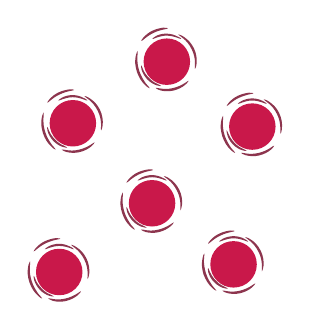
\begin{tikzpicture}[y=1cm, x=1cm,]
				\begin{scope}[shift={(10.7245, -0.7761)}]
					\path[draw=black,fill=cc9184a,draw opacity=0.0,line width=0.1054cm,miter limit=10.0,cm={ 0.1,-0.0,-0.0,-0.1,(-10.7245, 1.3336)}] (113.4154, -39.3133).. controls (113.4154, -37.6817) and (112.0938, -36.3615) .. (110.4636, -36.3615).. controls (108.8348, -36.3615) and (107.5132, -37.6817) .. (107.5132, -39.3133).. controls (107.5132, -40.9421) and (108.8348, -42.2637) .. (110.4636, -42.2637).. controls (112.0938, -42.2637) and (113.4154, -40.9421) .. (113.4154, -39.3133) -- cycle(113.4154, -39.3133);

				\end{scope}
				\begin{scope}[shift={(10.6186, -0.635)}]
					\path[fill=c8d354e] (0.4425, 5.5475).. controls (0.4425, 5.5433) and (0.4214, 5.5391) .. (0.3878, 5.5327).. controls (0.354, 5.5243) and (0.3077, 5.5138) .. (0.2613, 5.4906).. controls (0.1665, 5.4463) and (0.1116, 5.3788) .. (0.1032, 5.3873).. controls (0.101, 5.3894) and (0.1116, 5.4105) .. (0.1348, 5.4358).. controls (0.1454, 5.4484) and (0.1643, 5.4631) .. (0.1812, 5.478).. controls (0.2001, 5.4928) and (0.2232, 5.5074) .. (0.2465, 5.518).. controls (0.2971, 5.5413) and (0.3477, 5.5517) .. (0.3814, 5.5559).. controls (0.4193, 5.5559) and (0.4425, 5.5517) .. (0.4425, 5.5475) -- cycle(0.4425, 5.5475);

					\path[fill=c8d354e] (0.0568, 5.2608).. controls (0.061, 5.2586) and (0.0568, 5.2312) .. (0.0547, 5.1849).. controls (0.0547, 5.1724) and (0.0547, 5.1618) .. (0.0547, 5.147).. controls (0.0547, 5.1343) and (0.0547, 5.1175) .. (0.0568, 5.1028).. controls (0.061, 5.0711) and (0.0674, 5.0395) .. (0.078, 5.0078).. controls (0.0885, 4.9741) and (0.1032, 4.9446) .. (0.118, 4.9173).. controls (0.1264, 4.9045) and (0.1327, 4.8919) .. (0.1412, 4.8793).. controls (0.1495, 4.8688) and (0.1579, 4.8582) .. (0.1622, 4.8476).. controls (0.1917, 4.8119) and (0.2128, 4.7929) .. (0.2107, 4.7865).. controls (0.2086, 4.7844) and (0.1812, 4.7971) .. (0.1475, 4.833).. controls (0.139, 4.8412) and (0.1284, 4.8518) .. (0.12, 4.8623).. controls (0.1096, 4.8729) and (0.101, 4.8856) .. (0.0927, 4.9003).. controls (0.0758, 4.9278) and (0.061, 4.9593) .. (0.0484, 4.9951).. controls (0.0378, 5.031) and (0.0295, 5.0669) .. (0.0273, 5.0985).. controls (0.0273, 5.1153) and (0.0273, 5.1302) .. (0.0273, 5.1427).. controls (0.0273, 5.1575) and (0.0295, 5.1702) .. (0.0314, 5.1828).. controls (0.0314, 5.1955) and (0.0358, 5.206) .. (0.0378, 5.2145).. controls (0.04, 5.2229) and (0.0442, 5.2312) .. (0.0463, 5.2377).. controls (0.0506, 5.2545) and (0.0547, 5.2608) .. (0.0568, 5.2608) -- cycle(0.0568, 5.2608);

					\path[fill=c8d354e] (0.2865, 4.7908).. controls (0.2865, 4.7949) and (0.3141, 4.7886) .. (0.352, 4.7824).. controls (0.3919, 4.776) and (0.4468, 4.7738) .. (0.5057, 4.7886).. controls (0.5649, 4.8013) and (0.6134, 4.8266) .. (0.6491, 4.8476).. controls (0.6849, 4.8688) and (0.7018, 4.8856) .. (0.7039, 4.8813).. controls (0.706, 4.8793) and (0.6934, 4.8582) .. (0.6597, 4.8287).. controls (0.6281, 4.8013) and (0.5753, 4.7718) .. (0.5121, 4.757).. controls (0.4488, 4.7423) and (0.3878, 4.7486) .. (0.3477, 4.7591).. controls (0.3077, 4.7718) and (0.2844, 4.7865) .. (0.2865, 4.7908) -- cycle(0.7862, 5.0332).. controls (0.7819, 5.0332) and (0.7862, 5.0647) .. (0.7862, 5.1091).. controls (0.7862, 5.1554) and (0.7756, 5.2207) .. (0.744, 5.2819).. controls (0.7145, 5.3452) and (0.6701, 5.3937) .. (0.6343, 5.421).. controls (0.5986, 5.4506) and (0.5733, 5.4653) .. (0.5753, 5.4695).. controls (0.5753, 5.4717) and (0.6069, 5.4653) .. (0.6471, 5.4379).. controls (0.6682, 5.4252) and (0.6892, 5.4042) .. (0.7123, 5.3831).. controls (0.7334, 5.3599) and (0.7545, 5.3282) .. (0.7714, 5.2967).. controls (0.8052, 5.2271) and (0.8114, 5.1575) .. (0.8073, 5.1091).. controls (0.803, 5.0606) and (0.7903, 5.0332) .. (0.7862, 5.0332) -- cycle(0.1032, 5.0774).. controls (0.1073, 5.0795) and (0.1137, 5.0584) .. (0.1264, 5.0268).. controls (0.139, 4.9951) and (0.1643, 4.9552) .. (0.2001, 4.9194).. controls (0.2339, 4.8813) and (0.274, 4.8561) .. (0.3055, 4.8434).. controls (0.335, 4.8266) and (0.3562, 4.8203) .. (0.3562, 4.816).. controls (0.3562, 4.8139) and (0.3329, 4.8119) .. (0.2971, 4.8245).. controls (0.2633, 4.835) and (0.217, 4.8604) .. (0.179, 4.9003).. controls (0.1412, 4.9404) and (0.118, 4.9867) .. (0.1073, 5.0226).. controls (0.0989, 5.0543) and (0.101, 5.0754) .. (0.1032, 5.0774) -- cycle(0.1032, 5.0774);

					\path[fill=c8d354e] (0.6112, 5.4126).. controls (0.6091, 5.4084) and (0.5901, 5.4189) .. (0.5584, 5.4295).. controls (0.5501, 5.4316) and (0.5417, 5.4358) .. (0.5311, 5.4379).. controls (0.5206, 5.44) and (0.51, 5.4443) .. (0.4995, 5.4463).. controls (0.4785, 5.4506) and (0.4552, 5.4547) .. (0.4277, 5.4547).. controls (0.4025, 5.4547) and (0.3772, 5.4527) .. (0.3562, 5.4463).. controls (0.3456, 5.4443) and (0.335, 5.442) .. (0.3245, 5.4379).. controls (0.3141, 5.4358) and (0.3055, 5.4316) .. (0.2971, 5.4295).. controls (0.2655, 5.4168) and (0.2445, 5.4084) .. (0.2445, 5.4126).. controls (0.2423, 5.4148) and (0.2571, 5.4316) .. (0.2887, 5.4484).. controls (0.2971, 5.4527) and (0.3055, 5.4569) .. (0.3161, 5.4611).. controls (0.3266, 5.4653) and (0.3371, 5.4695) .. (0.3477, 5.4717).. controls (0.3708, 5.478) and (0.3983, 5.4801) .. (0.4236, 5.4801).. controls (0.4488, 5.4801) and (0.4763, 5.4758) .. (0.4995, 5.4695).. controls (0.51, 5.4674) and (0.5206, 5.4631) .. (0.5311, 5.4589).. controls (0.5417, 5.4569) and (0.5501, 5.4506) .. (0.5584, 5.4463).. controls (0.5986, 5.4316) and (0.6134, 5.4168) .. (0.6112, 5.4126) -- cycle(0.6112, 5.4126);

				\end{scope}
				\begin{scope}[shift={(9.525, -1.5522)}]
					\path[draw=black,fill=cc9184a,draw opacity=0.0,line width=0.1054cm,miter limit=10.0,cm={ 0.1,-0.0,-0.0,-0.1,(-9.525, 2.1098)}] (101.4843, -31.4915).. controls (101.4843, -29.8627) and (100.1628, -28.5411) .. (98.5339, -28.5411).. controls (96.9037, -28.5411) and (95.5822, -29.8627) .. (95.5822, -31.4915).. controls (95.5822, -33.1231) and (96.9037, -34.4433) .. (98.5339, -34.4433).. controls (100.1628, -34.4433) and (101.4843, -33.1231) .. (101.4843, -31.4915) -- cycle(101.4843, -31.4915);

				\end{scope}
				\begin{scope}[shift={(9.4192, -1.4111)}]
					\path[fill=c8d354e] (0.449, 5.5415).. controls (0.449, 5.5374) and (0.4279, 5.5331) .. (0.3941, 5.5268).. controls (0.3604, 5.5205) and (0.3139, 5.5057) .. (0.2676, 5.4846).. controls (0.1727, 5.4404) and (0.118, 5.373) .. (0.1096, 5.3793).. controls (0.1075, 5.3814) and (0.118, 5.4003) .. (0.1411, 5.4277).. controls (0.1517, 5.4404) and (0.1707, 5.4551) .. (0.1874, 5.4699).. controls (0.2066, 5.4846) and (0.2296, 5.4994) .. (0.2529, 5.51).. controls (0.3034, 5.5331) and (0.354, 5.5436) .. (0.3878, 5.5479).. controls (0.4257, 5.5499) and (0.449, 5.5458) .. (0.449, 5.5415) -- cycle(0.449, 5.5415);

					\path[fill=c8d354e] (0.0631, 5.2549).. controls (0.0674, 5.2549) and (0.0631, 5.2232) .. (0.061, 5.179).. controls (0.061, 5.1685) and (0.061, 5.1558) .. (0.061, 5.1411).. controls (0.061, 5.1284) and (0.061, 5.1115) .. (0.0631, 5.0989).. controls (0.0674, 5.0672) and (0.0737, 5.0357) .. (0.0842, 5.0041).. controls (0.0948, 4.9703) and (0.1096, 4.9409) .. (0.1242, 4.9134).. controls (0.1327, 4.9008) and (0.139, 4.8881) .. (0.1475, 4.8754).. controls (0.1559, 4.8649) and (0.1644, 4.8543) .. (0.1685, 4.8438).. controls (0.198, 4.808) and (0.2191, 4.789) .. (0.217, 4.7827).. controls (0.2148, 4.7806) and (0.1874, 4.7933) .. (0.1538, 4.8291).. controls (0.1452, 4.8375) and (0.1348, 4.848) .. (0.1264, 4.8586).. controls (0.1159, 4.8691) and (0.1075, 4.8817) .. (0.0989, 4.8965).. controls (0.0821, 4.9239) and (0.0674, 4.9556) .. (0.0547, 4.9914).. controls (0.0442, 5.0271) and (0.0357, 5.0631) .. (0.0336, 5.0948).. controls (0.0336, 5.1115) and (0.0336, 5.1263) .. (0.0336, 5.1389).. controls (0.0336, 5.1536) and (0.0357, 5.1663) .. (0.0379, 5.179).. controls (0.0379, 5.1896) and (0.042, 5.2021) .. (0.0442, 5.2107).. controls (0.0463, 5.2211) and (0.0504, 5.2275) .. (0.0526, 5.2338).. controls (0.0568, 5.2486) and (0.061, 5.2549) .. (0.0631, 5.2549) -- cycle(0.0631, 5.2549);

					\path[fill=c8d354e] (0.2928, 4.7847).. controls (0.2928, 4.789) and (0.3203, 4.7827) .. (0.3583, 4.7763).. controls (0.3983, 4.77) and (0.4531, 4.768) .. (0.5122, 4.7827).. controls (0.5712, 4.7953) and (0.6196, 4.8207) .. (0.6555, 4.8418).. controls (0.6914, 4.8629) and (0.7082, 4.8797) .. (0.7102, 4.8754).. controls (0.7124, 4.8733) and (0.6998, 4.8522) .. (0.666, 4.8228).. controls (0.6344, 4.7953) and (0.5817, 4.7658) .. (0.5186, 4.7511).. controls (0.4553, 4.7364) and (0.3941, 4.7426) .. (0.354, 4.7532).. controls (0.3139, 4.7658) and (0.2908, 4.7806) .. (0.2928, 4.7847) -- cycle(0.2928, 4.7847);

					\path[fill=c8d354e] (0.7925, 5.0271).. controls (0.7882, 5.0271) and (0.7925, 5.0588) .. (0.7925, 5.103).. controls (0.7925, 5.1495) and (0.782, 5.2148) .. (0.7503, 5.276).. controls (0.7188, 5.3391) and (0.6766, 5.3876) .. (0.6407, 5.4152).. controls (0.6048, 5.4445) and (0.5796, 5.4593) .. (0.5817, 5.4637).. controls (0.5817, 5.4656) and (0.6134, 5.4593) .. (0.6533, 5.432).. controls (0.6744, 5.4193) and (0.6955, 5.4003) .. (0.7188, 5.3771).. controls (0.7399, 5.3539) and (0.761, 5.3245) .. (0.7778, 5.2906).. controls (0.8115, 5.2211) and (0.8179, 5.1536) .. (0.8136, 5.103).. controls (0.8093, 5.0545) and (0.7968, 5.0271) .. (0.7925, 5.0271) -- cycle(0.7925, 5.0271);

					\path[fill=c8d354e] (0.1096, 5.0715).. controls (0.1137, 5.0715) and (0.12, 5.0504) .. (0.1327, 5.0209).. controls (0.1452, 4.9914) and (0.1707, 4.9493) .. (0.2066, 4.9134).. controls (0.2402, 4.8754) and (0.2803, 4.8502) .. (0.3119, 4.8375).. controls (0.3413, 4.8207) and (0.3624, 4.8144) .. (0.3624, 4.8101).. controls (0.3624, 4.808) and (0.3393, 4.8058) .. (0.3034, 4.8185).. controls (0.2697, 4.8291) and (0.2234, 4.8543) .. (0.1855, 4.8944).. controls (0.1475, 4.9345) and (0.1242, 4.9808) .. (0.1137, 5.0166).. controls (0.1053, 5.0482) and (0.1075, 5.0693) .. (0.1096, 5.0715) -- cycle(0.6175, 5.4066).. controls (0.6154, 5.4024) and (0.5964, 5.413) .. (0.5649, 5.4234).. controls (0.5563, 5.4256) and (0.5479, 5.4298) .. (0.5374, 5.432).. controls (0.527, 5.4341) and (0.5164, 5.4382) .. (0.5059, 5.4404).. controls (0.4848, 5.4445) and (0.4615, 5.4488) .. (0.4342, 5.4488).. controls (0.4089, 5.4488) and (0.3835, 5.4467) .. (0.3624, 5.4404).. controls (0.352, 5.4382) and (0.3413, 5.4361) .. (0.3309, 5.432).. controls (0.3203, 5.4298) and (0.3119, 5.4256) .. (0.3034, 5.4234).. controls (0.2717, 5.413) and (0.2507, 5.4024) .. (0.2507, 5.4066).. controls (0.2487, 5.4087) and (0.2633, 5.4256) .. (0.295, 5.4425).. controls (0.3034, 5.4467) and (0.3119, 5.4509) .. (0.3225, 5.4551).. controls (0.3329, 5.4593) and (0.3435, 5.4637) .. (0.354, 5.4656).. controls (0.3772, 5.472) and (0.4046, 5.4762) .. (0.4299, 5.4762).. controls (0.4553, 5.4762) and (0.4826, 5.472) .. (0.5059, 5.4656).. controls (0.5164, 5.4637) and (0.527, 5.4593) .. (0.5374, 5.4551).. controls (0.5479, 5.4531) and (0.5563, 5.4467) .. (0.5649, 5.4425).. controls (0.6048, 5.4256) and (0.6196, 5.4109) .. (0.6175, 5.4066) -- cycle(0.6175, 5.4066);

				\end{scope}
				\begin{scope}[shift={(11.8181, -1.5875)}]
					\path[draw=black,fill=cc9184a,draw opacity=0.0,line width=0.1054cm,miter limit=10.0,cm={ 0.1,-0.0,-0.0,-0.1,(-11.8181, 2.145)}] (124.2716, -31.0698).. controls (124.2716, -29.441) and (122.95, -28.1195) .. (121.3198, -28.1195).. controls (119.691, -28.1195) and (118.3694, -29.441) .. (118.3694, -31.0698).. controls (118.3694, -32.7014) and (119.691, -34.0216) .. (121.3198, -34.0216).. controls (122.95, -34.0216) and (124.2716, -32.7014) .. (124.2716, -31.0698) -- cycle(124.2716, -31.0698);

				\end{scope}
				\begin{scope}[shift={(11.7122, -1.4464)}]
					\path[fill=c8d354e] (0.4345, 5.5347).. controls (0.4345, 5.5305) and (0.4134, 5.5262) .. (0.3798, 5.5199).. controls (0.346, 5.5115) and (0.2996, 5.499) .. (0.2533, 5.4777).. controls (0.1585, 5.4335) and (0.1036, 5.3661) .. (0.0952, 5.3725).. controls (0.093, 5.3744) and (0.1036, 5.3935) .. (0.1268, 5.4208).. controls (0.1374, 5.4335) and (0.1563, 5.4482) .. (0.1731, 5.463).. controls (0.1921, 5.4777) and (0.2154, 5.4925) .. (0.2385, 5.5031).. controls (0.2891, 5.5262) and (0.3397, 5.5367) .. (0.3734, 5.541).. controls (0.4113, 5.5431) and (0.4345, 5.5389) .. (0.4345, 5.5347) -- cycle(0.4345, 5.5347);

					\path[fill=c8d354e] (0.0488, 5.248).. controls (0.0531, 5.248) and (0.0488, 5.2163) .. (0.0467, 5.1721).. controls (0.0467, 5.1616) and (0.0445, 5.1489) .. (0.0467, 5.1342).. controls (0.0467, 5.1215) and (0.0467, 5.1046) .. (0.0488, 5.092).. controls (0.0531, 5.0605) and (0.0594, 5.0288) .. (0.0699, 4.9972).. controls (0.0805, 4.9635) and (0.0952, 4.934) .. (0.11, 4.9065).. controls (0.1163, 4.8939) and (0.1247, 4.8812) .. (0.1331, 4.8685).. controls (0.1415, 4.858) and (0.1499, 4.8474) .. (0.1542, 4.837).. controls (0.1837, 4.8011) and (0.2048, 4.7822) .. (0.2026, 4.7758).. controls (0.2006, 4.7737) and (0.1753, 4.7864) .. (0.1393, 4.8222).. controls (0.1311, 4.8306) and (0.1226, 4.8411) .. (0.112, 4.8517).. controls (0.1036, 4.8622) and (0.0952, 4.8748) .. (0.0846, 4.8896).. controls (0.0678, 4.917) and (0.0531, 4.9487) .. (0.0404, 4.9845).. controls (0.0298, 5.0202) and (0.0214, 5.0562) .. (0.0193, 5.0879).. controls (0.0193, 5.1046) and (0.0193, 5.1194) .. (0.0193, 5.132).. controls (0.0193, 5.1467) and (0.0214, 5.1594) .. (0.0234, 5.1721).. controls (0.0234, 5.1827) and (0.0277, 5.1952) .. (0.0298, 5.2038).. controls (0.032, 5.2143) and (0.0361, 5.2206) .. (0.0383, 5.2269).. controls (0.0424, 5.2417) and (0.0467, 5.248) .. (0.0488, 5.248) -- cycle(0.0488, 5.248);

					\path[fill=c8d354e] (0.2785, 4.7778).. controls (0.2785, 4.7822) and (0.3059, 4.7758) .. (0.344, 4.7694).. controls (0.3839, 4.7631) and (0.4388, 4.7612) .. (0.4977, 4.7758).. controls (0.5567, 4.7884) and (0.6074, 4.8138) .. (0.6411, 4.8349).. controls (0.6748, 4.856) and (0.6938, 4.8728) .. (0.698, 4.8685).. controls (0.7002, 4.8664) and (0.6875, 4.8454) .. (0.6537, 4.8159).. controls (0.6222, 4.7884) and (0.5695, 4.759) .. (0.5063, 4.7442).. controls (0.443, 4.7295) and (0.3839, 4.7357) .. (0.3418, 4.7463).. controls (0.2996, 4.759) and (0.2764, 4.7737) .. (0.2785, 4.7778) -- cycle(0.7782, 5.0202).. controls (0.7739, 5.0202) and (0.7782, 5.0519) .. (0.7761, 5.0963).. controls (0.7761, 5.1426) and (0.7655, 5.2079) .. (0.7339, 5.2691).. controls (0.7043, 5.3324) and (0.6602, 5.3809) .. (0.6243, 5.4083).. controls (0.5884, 5.4376) and (0.5632, 5.4524) .. (0.5653, 5.4568).. controls (0.5673, 5.4587) and (0.597, 5.4524) .. (0.6369, 5.4251).. controls (0.658, 5.4124) and (0.6791, 5.3935) .. (0.7022, 5.3703).. controls (0.7254, 5.347) and (0.7444, 5.3176) .. (0.7612, 5.2838).. controls (0.795, 5.2143) and (0.8013, 5.1467) .. (0.7972, 5.0963).. controls (0.795, 5.0478) and (0.7823, 5.0202) .. (0.7782, 5.0202) -- cycle(0.0952, 5.0646).. controls (0.0994, 5.0646) and (0.1057, 5.0435) .. (0.1204, 5.014).. controls (0.1331, 4.9825) and (0.1585, 4.9424) .. (0.1921, 4.9065).. controls (0.2281, 4.8685) and (0.268, 4.8433) .. (0.2975, 4.8306).. controls (0.327, 4.8138) and (0.3481, 4.8075) .. (0.3481, 4.8033).. controls (0.346, 4.8011) and (0.3249, 4.7989) .. (0.2891, 4.8116).. controls (0.2554, 4.8222) and (0.2089, 4.8474) .. (0.171, 4.8875).. controls (0.1331, 4.9276) and (0.11, 4.9739) .. (0.1016, 5.0098).. controls (0.091, 5.0413) and (0.093, 5.0624) .. (0.0952, 5.0646) -- cycle(0.0952, 5.0646);

					\path[fill=c8d354e] (0.6032, 5.3997).. controls (0.6011, 5.3955) and (0.5821, 5.4061) .. (0.5504, 5.4167).. controls (0.542, 5.4188) and (0.5337, 5.4229) .. (0.5231, 5.4251).. controls (0.5126, 5.4272) and (0.502, 5.4313) .. (0.4915, 5.4335).. controls (0.4705, 5.4376) and (0.4472, 5.4419) .. (0.4198, 5.4419).. controls (0.3945, 5.4419) and (0.3692, 5.4398) .. (0.3481, 5.4335).. controls (0.3376, 5.4313) and (0.327, 5.4292) .. (0.3186, 5.4251).. controls (0.308, 5.4229) and (0.2996, 5.4188) .. (0.2913, 5.4167).. controls (0.2596, 5.4061) and (0.2385, 5.3955) .. (0.2363, 5.3997).. controls (0.2343, 5.4019) and (0.2511, 5.4188) .. (0.2828, 5.4356).. controls (0.2913, 5.4398) and (0.2996, 5.444) .. (0.3102, 5.4482).. controls (0.3207, 5.4524) and (0.3313, 5.4568) .. (0.3418, 5.4587).. controls (0.365, 5.4651) and (0.3923, 5.4693) .. (0.4198, 5.4693).. controls (0.4472, 5.4693) and (0.4725, 5.4651) .. (0.4957, 5.4587).. controls (0.5063, 5.4568) and (0.5168, 5.4524) .. (0.5274, 5.4482).. controls (0.5378, 5.4462) and (0.5463, 5.4398) .. (0.5548, 5.4356).. controls (0.5905, 5.4188) and (0.6052, 5.404) .. (0.6032, 5.3997) -- cycle(0.6032, 5.3997);

				\end{scope}
				\begin{scope}[shift={(10.5481, -2.5753)}]
					\path[draw=black,fill=cc9184a,draw opacity=0.0,line width=0.1054cm,miter limit=10.0,cm={ 0.1,-0.0,-0.0,-0.1,(-10.5481, 3.1328)}] (111.5399, -21.3312).. controls (111.5399, -19.7024) and (110.2183, -18.3809) .. (108.5881, -18.3809).. controls (106.9579, -18.3809) and (105.6377, -19.7024) .. (105.6377, -21.3312).. controls (105.6377, -22.9615) and (106.9579, -24.283) .. (108.5881, -24.283).. controls (110.2183, -24.283) and (111.5399, -22.9615) .. (111.5399, -21.3312) -- cycle(111.5399, -21.3312);

				\end{scope}
				\begin{scope}[shift={(10.407, -2.4342)}]
					\path[fill=c8d354e] (0.4666, 5.5486).. controls (0.4666, 5.5443) and (0.4455, 5.5402) .. (0.4118, 5.5338).. controls (0.3781, 5.5275) and (0.3317, 5.5127) .. (0.2853, 5.4917).. controls (0.1904, 5.4474) and (0.1357, 5.38) .. (0.1272, 5.3862).. controls (0.1251, 5.3884) and (0.1357, 5.4073) .. (0.1589, 5.4347).. controls (0.1694, 5.4474) and (0.1884, 5.4622) .. (0.2053, 5.4769).. controls (0.2242, 5.4917) and (0.2475, 5.5064) .. (0.2705, 5.517).. controls (0.3212, 5.5402) and (0.3718, 5.5506) .. (0.4056, 5.5549).. controls (0.4455, 5.557) and (0.4666, 5.5528) .. (0.4666, 5.5486) -- cycle(0.4666, 5.5486);

					\path[fill=c8d354e] (0.0808, 5.2619).. controls (0.085, 5.2619) and (0.0808, 5.2302) .. (0.0788, 5.186).. controls (0.0788, 5.1754) and (0.0788, 5.1629) .. (0.0788, 5.1481).. controls (0.0788, 5.1354) and (0.0788, 5.1185) .. (0.0808, 5.1059).. controls (0.085, 5.0744) and (0.0914, 5.0427) .. (0.102, 5.0111).. controls (0.1124, 4.9774) and (0.1272, 4.9479) .. (0.1421, 4.9205).. controls (0.1505, 4.9078) and (0.1568, 4.8951) .. (0.1652, 4.8824).. controls (0.1736, 4.872) and (0.182, 4.8613) .. (0.1862, 4.8509).. controls (0.2158, 4.815) and (0.2369, 4.796) .. (0.2347, 4.7898).. controls (0.2326, 4.7876) and (0.2053, 4.8003) .. (0.1714, 4.8361).. controls (0.1632, 4.8445) and (0.1525, 4.855) .. (0.1441, 4.8656).. controls (0.1335, 4.8761) and (0.1251, 4.8888) .. (0.1167, 4.9035).. controls (0.0999, 4.9309) and (0.085, 4.9626) .. (0.0725, 4.9985).. controls (0.0619, 5.0343) and (0.0535, 5.07) .. (0.0514, 5.1017).. controls (0.0514, 5.1185) and (0.0514, 5.1332) .. (0.0514, 5.1459).. controls (0.0514, 5.1607) and (0.0535, 5.1733) .. (0.0555, 5.186).. controls (0.0555, 5.1965) and (0.0598, 5.2092) .. (0.0619, 5.2176).. controls (0.0639, 5.2282) and (0.0682, 5.2345) .. (0.0703, 5.2409).. controls (0.0766, 5.2556) and (0.0788, 5.2619) .. (0.0808, 5.2619) -- cycle(0.0808, 5.2619);

					\path[fill=c8d354e] (0.3106, 4.7918).. controls (0.3106, 4.796) and (0.338, 4.7898) .. (0.3759, 4.7833).. controls (0.416, 4.777) and (0.4709, 4.7749) .. (0.5299, 4.7898).. controls (0.5888, 4.8024) and (0.6373, 4.8276) .. (0.6732, 4.8487).. controls (0.709, 4.8697) and (0.726, 4.8867) .. (0.728, 4.8824).. controls (0.7301, 4.8804) and (0.7174, 4.8593) .. (0.6838, 4.8298).. controls (0.6521, 4.8024) and (0.5994, 4.7729) .. (0.5362, 4.7581).. controls (0.4729, 4.7432) and (0.4118, 4.7496) .. (0.3718, 4.7602).. controls (0.3317, 4.7729) and (0.3106, 4.7876) .. (0.3106, 4.7918) -- cycle(0.3106, 4.7918);

					\path[fill=c8d354e] (0.8122, 5.0343).. controls (0.8081, 5.0343) and (0.8122, 5.0658) .. (0.8122, 5.1101).. controls (0.8122, 5.1565) and (0.8017, 5.2218) .. (0.77, 5.283).. controls (0.7385, 5.3463) and (0.6963, 5.3948) .. (0.6605, 5.4222).. controls (0.6248, 5.4516) and (0.5994, 5.4663) .. (0.6015, 5.4706).. controls (0.6015, 5.4726) and (0.6331, 5.4663) .. (0.6732, 5.4389).. controls (0.6943, 5.4263) and (0.7153, 5.4073) .. (0.7385, 5.3842).. controls (0.7596, 5.361) and (0.7807, 5.3315) .. (0.7975, 5.2978).. controls (0.8314, 5.2282) and (0.8377, 5.1607) .. (0.8333, 5.1101).. controls (0.8271, 5.0617) and (0.8144, 5.0343) .. (0.8122, 5.0343) -- cycle(0.8122, 5.0343);

					\path[fill=c8d354e] (0.1293, 5.0785).. controls (0.1335, 5.0785) and (0.1399, 5.0574) .. (0.1525, 5.0278).. controls (0.1652, 4.9985) and (0.1904, 4.9563) .. (0.2263, 4.9205).. controls (0.26, 4.8824) and (0.3001, 4.8572) .. (0.3317, 4.8445).. controls (0.3612, 4.8276) and (0.3823, 4.8214) .. (0.3823, 4.8171).. controls (0.3823, 4.815) and (0.3591, 4.8128) .. (0.3233, 4.8255).. controls (0.2897, 4.8361) and (0.2431, 4.8613) .. (0.2053, 4.9014).. controls (0.1673, 4.9415) and (0.1441, 4.9878) .. (0.1335, 5.0237).. controls (0.1251, 5.0552) and (0.1251, 5.0763) .. (0.1293, 5.0785) -- cycle(0.6373, 5.4137).. controls (0.6353, 5.4094) and (0.6164, 5.42) .. (0.5847, 5.4305).. controls (0.5763, 5.4327) and (0.5679, 5.4368) .. (0.5573, 5.4389).. controls (0.5467, 5.4411) and (0.5362, 5.4452) .. (0.5257, 5.4474).. controls (0.5046, 5.4516) and (0.4813, 5.4558) .. (0.4539, 5.4558).. controls (0.4287, 5.4558) and (0.4034, 5.4538) .. (0.3823, 5.4474).. controls (0.3718, 5.4452) and (0.3612, 5.4433) .. (0.3507, 5.4389).. controls (0.3401, 5.4368) and (0.3317, 5.4327) .. (0.3233, 5.4305).. controls (0.2916, 5.42) and (0.2705, 5.4094) .. (0.2705, 5.4137).. controls (0.2684, 5.4159) and (0.2832, 5.4327) .. (0.3149, 5.4495).. controls (0.3233, 5.4538) and (0.3317, 5.4579) .. (0.3423, 5.4622).. controls (0.3529, 5.4663) and (0.3634, 5.4706) .. (0.3739, 5.4726).. controls (0.397, 5.479) and (0.4244, 5.4833) .. (0.4497, 5.4833).. controls (0.475, 5.4833) and (0.5024, 5.479) .. (0.5257, 5.4726).. controls (0.5362, 5.4706) and (0.5467, 5.4663) .. (0.5573, 5.4622).. controls (0.5679, 5.46) and (0.5763, 5.4538) .. (0.5847, 5.4495).. controls (0.6226, 5.4327) and (0.6394, 5.4178) .. (0.6373, 5.4137) -- cycle(0.6373, 5.4137);

				\end{scope}
				\begin{scope}[shift={(11.5711, -3.3514)}]
					\path[draw=black,fill=cc9184a,draw opacity=0.0,line width=0.1054cm,miter limit=10.0,cm={ 0.1,-0.0,-0.0,-0.1,(-11.5711, 3.9089)}] (121.8889, -13.5743).. controls (121.8889, -11.9454) and (120.5688, -10.6239) .. (118.9372, -10.6239).. controls (117.3083, -10.6239) and (115.9868, -11.9454) .. (115.9868, -13.5743).. controls (115.9868, -15.2045) and (117.3083, -16.526) .. (118.9372, -16.526).. controls (120.5688, -16.526) and (121.8889, -15.2045) .. (121.8889, -13.5743) -- cycle(121.8889, -13.5743);

				\end{scope}
				\begin{scope}[shift={(11.4653, -3.2103)}]
					\path[fill=c8d354e] (0.4433, 5.549).. controls (0.4433, 5.5448) and (0.4222, 5.5404) .. (0.3885, 5.5342).. controls (0.3547, 5.5257) and (0.3084, 5.5132) .. (0.2642, 5.4921).. controls (0.1694, 5.4478) and (0.1123, 5.3803) .. (0.1061, 5.3867).. controls (0.1017, 5.3887) and (0.1123, 5.4077) .. (0.1377, 5.4352).. controls (0.1483, 5.4478) and (0.165, 5.4626) .. (0.1841, 5.4772).. controls (0.203, 5.4921) and (0.2261, 5.5068) .. (0.2515, 5.5174).. controls (0.3, 5.5404) and (0.3526, 5.5511) .. (0.3863, 5.5553).. controls (0.4222, 5.5574) and (0.4433, 5.5531) .. (0.4433, 5.549) -- cycle(0.4433, 5.549);

					\path[fill=c8d354e] (0.0576, 5.2622).. controls (0.0617, 5.2622) and (0.0554, 5.2307) .. (0.0533, 5.1864).. controls (0.0533, 5.1759) and (0.0533, 5.1633) .. (0.0533, 5.1485).. controls (0.0533, 5.1358) and (0.0533, 5.1189) .. (0.0576, 5.1064).. controls (0.0617, 5.0747) and (0.0681, 5.0431) .. (0.0787, 5.0114).. controls (0.0892, 4.9776) and (0.1039, 4.9482) .. (0.1186, 4.9207).. controls (0.1272, 4.9081) and (0.1334, 4.8955) .. (0.1418, 4.8828).. controls (0.1483, 4.8722) and (0.1588, 4.8618) .. (0.1629, 4.8511).. controls (0.1903, 4.8155) and (0.2135, 4.7964) .. (0.2114, 4.7901).. controls (0.2093, 4.788) and (0.1819, 4.8007) .. (0.1483, 4.8365).. controls (0.1397, 4.8448) and (0.1291, 4.8554) .. (0.1209, 4.8659).. controls (0.1102, 4.8765) and (0.1017, 4.8892) .. (0.0933, 4.9039).. controls (0.0765, 4.9313) and (0.0617, 4.9629) .. (0.047, 4.9987).. controls (0.0365, 5.0346) and (0.0302, 5.0705) .. (0.028, 5.1021).. controls (0.0259, 5.1189) and (0.0259, 5.1338) .. (0.028, 5.1463).. controls (0.028, 5.1611) and (0.0302, 5.1737) .. (0.0322, 5.1864).. controls (0.0343, 5.197) and (0.0365, 5.2096) .. (0.0386, 5.2181).. controls (0.0407, 5.2286) and (0.0449, 5.2348) .. (0.0449, 5.2411).. controls (0.0533, 5.2559) and (0.0554, 5.2622) .. (0.0576, 5.2622) -- cycle(0.0576, 5.2622);

					\path[fill=c8d354e] (0.2873, 4.7922).. controls (0.2873, 4.7964) and (0.3147, 4.7901) .. (0.3526, 4.7838).. controls (0.3907, 4.7774) and (0.4476, 4.7754) .. (0.5066, 4.7901).. controls (0.5655, 4.8028) and (0.6141, 4.8281) .. (0.6499, 4.8492).. controls (0.6836, 4.8703) and (0.7025, 4.887) .. (0.7047, 4.8828).. controls (0.7089, 4.8808) and (0.6941, 4.8597) .. (0.6604, 4.8302).. controls (0.6288, 4.8028) and (0.576, 4.7733) .. (0.5128, 4.7585).. controls (0.4495, 4.7438) and (0.3885, 4.75) .. (0.3485, 4.7606).. controls (0.3084, 4.7733) and (0.2873, 4.788) .. (0.2873, 4.7922) -- cycle(0.2873, 4.7922);

					\path[fill=c8d354e] (0.7889, 5.0346).. controls (0.7848, 5.0346) and (0.7889, 5.0663) .. (0.7889, 5.1105).. controls (0.7889, 5.1569) and (0.7785, 5.2223) .. (0.7469, 5.2833).. controls (0.7152, 5.3465) and (0.673, 5.3951) .. (0.6372, 5.4225).. controls (0.6014, 5.452) and (0.576, 5.4667) .. (0.5782, 5.471).. controls (0.5782, 5.4731) and (0.6098, 5.4667) .. (0.6499, 5.4394).. controls (0.671, 5.4268) and (0.6941, 5.4077) .. (0.7152, 5.3846).. controls (0.7363, 5.3613) and (0.7574, 5.3318) .. (0.7743, 5.298).. controls (0.8079, 5.2286) and (0.8143, 5.1611) .. (0.8101, 5.1105).. controls (0.8037, 5.062) and (0.7911, 5.0346) .. (0.7889, 5.0346) -- cycle(0.1061, 5.0789).. controls (0.1102, 5.0789) and (0.1166, 5.0579) .. (0.1291, 5.0284).. controls (0.1439, 4.9967) and (0.1672, 4.9566) .. (0.203, 4.9207).. controls (0.2367, 4.8828) and (0.2767, 4.8576) .. (0.3084, 4.8448).. controls (0.3379, 4.8281) and (0.359, 4.8218) .. (0.3569, 4.8175).. controls (0.3569, 4.8155) and (0.3336, 4.8132) .. (0.2978, 4.8259).. controls (0.2642, 4.8365) and (0.2177, 4.8618) .. (0.1798, 4.9019).. controls (0.1397, 4.9418) and (0.1186, 4.9883) .. (0.108, 5.0241).. controls (0.1017, 5.0556) and (0.1017, 5.0767) .. (0.1061, 5.0789) -- cycle(0.1061, 5.0789);

					\path[fill=c8d354e] (0.6141, 5.4141).. controls (0.612, 5.4098) and (0.593, 5.4204) .. (0.5613, 5.4309).. controls (0.5529, 5.4331) and (0.5445, 5.4372) .. (0.5339, 5.4394).. controls (0.5234, 5.4415) and (0.5128, 5.4456) .. (0.5023, 5.4478).. controls (0.4812, 5.452) and (0.4559, 5.4561) .. (0.4306, 5.4561).. controls (0.4054, 5.4561) and (0.3821, 5.4542) .. (0.359, 5.4478).. controls (0.3485, 5.4456) and (0.3379, 5.4436) .. (0.3274, 5.4394).. controls (0.3168, 5.4372) and (0.3105, 5.4331) .. (0.3, 5.4309).. controls (0.2683, 5.4204) and (0.2472, 5.4098) .. (0.2472, 5.4141).. controls (0.2452, 5.4161) and (0.2599, 5.4331) .. (0.2915, 5.4499).. controls (0.3, 5.4542) and (0.3084, 5.4583) .. (0.3189, 5.4626).. controls (0.3295, 5.4667) and (0.34, 5.471) .. (0.3526, 5.4731).. controls (0.3758, 5.4794) and (0.4011, 5.4837) .. (0.4284, 5.4837).. controls (0.4559, 5.4837) and (0.4812, 5.4794) .. (0.5066, 5.4731).. controls (0.517, 5.471) and (0.5277, 5.4667) .. (0.5383, 5.4626).. controls (0.5487, 5.4605) and (0.5571, 5.4542) .. (0.5655, 5.4499).. controls (0.5993, 5.4331) and (0.6161, 5.4183) .. (0.6141, 5.4141) -- cycle(0.6141, 5.4141);

				\end{scope}
				\begin{scope}[shift={(9.3486, -3.4219)}]
					\path[fill=cc9184a,draw opacity=0.0] (0.6269, 5.24).. controls (0.6269, 5.077) and (0.4949, 4.9449) .. (0.3318, 4.9449).. controls (0.1688, 4.9449) and (0.0367, 5.077) .. (0.0367, 5.24).. controls (0.0367, 5.4029) and (0.1688, 5.5351) .. (0.3318, 5.5351).. controls (0.4949, 5.5351) and (0.6269, 5.4029) .. (0.6269, 5.24) -- cycle(0.6269, 5.24);

					\path[draw=black,draw opacity=0.0,line width=0.1054cm,miter limit=10.0,cm={ 0.1,-0.0,-0.0,-0.1,(-9.3486, 3.9795)}] (99.7549, -12.6055).. controls (99.7549, -10.9753) and (98.4347, -9.6537) .. (96.8045, -9.6537).. controls (95.1743, -9.6537) and (93.8527, -10.9753) .. (93.8527, -12.6055).. controls (93.8527, -14.2343) and (95.1743, -15.5559) .. (96.8045, -15.5559).. controls (98.4347, -15.5559) and (99.7549, -14.2343) .. (99.7549, -12.6055) -- cycle(99.7549, -12.6055);

				\end{scope}
				\begin{scope}[shift={(9.2428, -3.3161)}]
					\path[fill=c8d354e] (0.4524, 5.5578).. controls (0.4524, 5.5537) and (0.4315, 5.5494) .. (0.3976, 5.5431).. controls (0.3638, 5.5367) and (0.3175, 5.522) .. (0.2712, 5.5009).. controls (0.1763, 5.4567) and (0.1214, 5.3891) .. (0.113, 5.3955).. controls (0.1109, 5.3977) and (0.1214, 5.4166) .. (0.1447, 5.444).. controls (0.1552, 5.4567) and (0.1742, 5.4714) .. (0.191, 5.4861).. controls (0.21, 5.5009) and (0.2332, 5.5156) .. (0.2565, 5.5262).. controls (0.307, 5.5494) and (0.3576, 5.56) .. (0.3912, 5.5641).. controls (0.4315, 5.5641) and (0.4524, 5.56) .. (0.4524, 5.5578) -- cycle(0.4524, 5.5578);

					\path[fill=c8d354e] (0.0667, 5.2691).. controls (0.071, 5.2691) and (0.0667, 5.2374) .. (0.0645, 5.1932).. controls (0.0645, 5.1826) and (0.0645, 5.17) .. (0.0645, 5.1553).. controls (0.0645, 5.1426) and (0.0645, 5.1256) .. (0.0667, 5.1131).. controls (0.071, 5.0814) and (0.0772, 5.0499) .. (0.0878, 5.0183).. controls (0.0983, 4.9844) and (0.113, 4.955) .. (0.1277, 4.9276).. controls (0.1363, 4.9149) and (0.1425, 4.9023) .. (0.151, 4.8896).. controls (0.1594, 4.8791) and (0.1678, 4.8685) .. (0.1721, 4.858).. controls (0.2016, 4.8222) and (0.2227, 4.8032) .. (0.2206, 4.7968).. controls (0.2184, 4.7948) and (0.191, 4.8075) .. (0.1574, 4.8433).. controls (0.1488, 4.8517) and (0.1384, 4.8622) .. (0.1299, 4.8728).. controls (0.1195, 4.8833) and (0.1109, 4.8959) .. (0.1025, 4.9107).. controls (0.0856, 4.9381) and (0.071, 4.9698) .. (0.0582, 5.0055).. controls (0.0477, 5.0413) and (0.0393, 5.0771) .. (0.0371, 5.1088).. controls (0.0371, 5.1256) and (0.0371, 5.1404) .. (0.0371, 5.1531).. controls (0.0371, 5.1678) and (0.0393, 5.1805) .. (0.0415, 5.1932).. controls (0.0415, 5.2036) and (0.0456, 5.2163) .. (0.0477, 5.2247).. controls (0.0497, 5.2352) and (0.054, 5.2417) .. (0.0562, 5.248).. controls (0.0626, 5.2628) and (0.0645, 5.2691) .. (0.0667, 5.2691) -- cycle(0.0667, 5.2691);

					\path[fill=c8d354e] (0.2964, 4.7989).. controls (0.2964, 4.8032) and (0.3238, 4.7968) .. (0.3619, 4.7905).. controls (0.4018, 4.7842) and (0.4567, 4.7821) .. (0.5157, 4.7968).. controls (0.5746, 4.8095) and (0.6231, 4.8347) .. (0.659, 4.8558).. controls (0.6949, 4.8769) and (0.7116, 4.8939) .. (0.7138, 4.8896).. controls (0.716, 4.8875) and (0.7034, 4.8664) .. (0.6696, 4.837).. controls (0.6379, 4.8095) and (0.5853, 4.78) .. (0.522, 4.7653).. controls (0.4587, 4.7504) and (0.3976, 4.7567) .. (0.3576, 4.7674).. controls (0.3175, 4.7821) and (0.2964, 4.7968) .. (0.2964, 4.7989) -- cycle(0.2964, 4.7989);

					\path[fill=c8d354e] (0.7982, 5.0435).. controls (0.7939, 5.0435) and (0.7982, 5.0751) .. (0.7982, 5.1193).. controls (0.7982, 5.1658) and (0.7875, 5.2311) .. (0.756, 5.2923).. controls (0.7243, 5.3555) and (0.6823, 5.4039) .. (0.6464, 5.4313).. controls (0.6106, 5.4609) and (0.5853, 5.4757) .. (0.5873, 5.4798).. controls (0.5873, 5.482) and (0.619, 5.4757) .. (0.659, 5.4482).. controls (0.6801, 5.4356) and (0.7011, 5.4166) .. (0.7243, 5.3934).. controls (0.7455, 5.3703) and (0.7665, 5.3406) .. (0.7834, 5.307).. controls (0.817, 5.2374) and (0.8234, 5.17) .. (0.8192, 5.1193).. controls (0.8129, 5.0709) and (0.8004, 5.0413) .. (0.7982, 5.0435) -- cycle(0.7982, 5.0435);

					\path[fill=c8d354e] (0.1152, 5.0857).. controls (0.1195, 5.0857) and (0.1257, 5.0646) .. (0.1384, 5.035).. controls (0.151, 5.0034) and (0.1763, 4.9635) .. (0.2121, 4.9276).. controls (0.2458, 4.8896) and (0.2859, 4.8644) .. (0.3175, 4.8517).. controls (0.3471, 4.8347) and (0.3682, 4.8285) .. (0.3682, 4.8243).. controls (0.3682, 4.8222) and (0.3449, 4.82) .. (0.3091, 4.8327).. controls (0.2753, 4.8433) and (0.229, 4.8685) .. (0.191, 4.9086).. controls (0.1531, 4.9487) and (0.1299, 4.995) .. (0.1195, 5.0308).. controls (0.1109, 5.0624) and (0.1109, 5.0857) .. (0.1152, 5.0857) -- cycle(0.6231, 5.4229).. controls (0.6211, 5.4188) and (0.6021, 5.4292) .. (0.5705, 5.4398).. controls (0.5621, 5.4419) and (0.5536, 5.446) .. (0.5431, 5.4482).. controls (0.5325, 5.4503) and (0.522, 5.4546) .. (0.5114, 5.4567).. controls (0.4903, 5.4609) and (0.4672, 5.4651) .. (0.4397, 5.4651).. controls (0.4145, 5.4651) and (0.3893, 5.463) .. (0.3682, 5.4567).. controls (0.3576, 5.4546) and (0.3471, 5.4524) .. (0.3365, 5.4482).. controls (0.326, 5.446) and (0.3175, 5.4419) .. (0.3091, 5.4398).. controls (0.2775, 5.4292) and (0.2565, 5.4188) .. (0.2565, 5.4229).. controls (0.2542, 5.425) and (0.269, 5.4419) .. (0.3006, 5.4587).. controls (0.3091, 5.463) and (0.3175, 5.4671) .. (0.3281, 5.4714).. controls (0.3386, 5.4757) and (0.3491, 5.4798) .. (0.3597, 5.482).. controls (0.383, 5.4882) and (0.4104, 5.4925) .. (0.4356, 5.4925).. controls (0.4608, 5.4925) and (0.4882, 5.4882) .. (0.5114, 5.482).. controls (0.522, 5.4798) and (0.5325, 5.4757) .. (0.5431, 5.4714).. controls (0.5536, 5.4693) and (0.5621, 5.463) .. (0.5705, 5.4587).. controls (0.6084, 5.4419) and (0.6254, 5.425) .. (0.6231, 5.4229) -- cycle(0.6231, 5.4229);

				\end{scope}

			\end{tikzpicture}
		\end{center}
	\end{minipage}

\end{qq}
\vspace{5pt}
\begin{minipage}{5cm}
	\begin{center}
		$\underline{\text{Solid}}$
	\end{center}
\end{minipage}
\begin{minipage}{5cm}
	\begin{center}
		$\underline{\text{Liquid}}$
	\end{center}
\end{minipage}
\begin{minipage}{5cm}
	\begin{center}
		$\underline{\text{Gas}}$
	\end{center}
\end{minipage}

\vspace{10pt}
\noindent \textbf{Inter-particle Forces} - We all know the 3 common states of matter, solid, liquid and gas. The temperatures at which a substance will be in one of these phases is dictated by the strength of the inter-particle forces between them. As the overall energy of the system increases, these are overcome, and the particles are allowed to move more freely. \\
\\
\textbf{Pressure} - Pressure, temperature, and volume are all directly related. When there is a difference in pressure between the inside and outside of a system, the area of greater pressure will exert a crushing force onto the area of lower pressure. \\
\\
\textbf{General Gas Properties}

{                                     % new code: create a group
	\setlength{\leftmargini}{1.5cm}         % new code: set margin length to 0 
	\begin{itemize}
		\item Highly compressible (Boyle's Law)
		\item Thermally expandable (Charles' Law)
		\item Low viscosity (flow easily)
		\item Low density (low mass per unit space)
		\item Infinitely miscible (unlimited ability to be mixed)
	\end{itemize}
}

\noindent\textbf{Volumetric Molecular Proportionality} - One thing to note is that the number of moles of a substances is directly proportional to its volume, regardless of the substance.\\
\\
\textbf{Ideal Gas Law} - Putting all the individual gas laws together gives us the ideal gas law, a statement about the relationship between volume, pressure, temperature, and amount of gas.
\begin{qq}

	\begin{center}
		$\text{\textcolor{red3}{$V$}}=\frac{\text{\textcolor{red4}{$n$}}\text{\textcolor{red5}{$R$}}\text{\textcolor{red1}{$T$}}}{\text{\textcolor{red2}{$p$}}} \quad \text{\textcolor{red2}{$p$}}=\frac{\text{\textcolor{red4}{$n$}}\text{\textcolor{red5}{$R$}}      \text{\textcolor{red1}{$T$}}}{\text{\textcolor{red3}{$V$}}}\quad \text{\textcolor{red1}{$T$}}=\frac{\text{\textcolor{red2}{$p$}}\text{\textcolor{red3}{$V$}}}{\text{\textcolor{red4}{$n$}}\text{\textcolor{red5}{$R$}}}\quad \text{\textcolor{red4}{$n$}}=\frac{\text{\textcolor{red3}{$V$}}\text{\textcolor{red2}{$p$}}}{\text{\textcolor{red5}{$R$}}\text{\textcolor{red1}{$T$}}}$\\
		\vspace{5pt}
		\small $\text{\textcolor{red3}{$V$}}=$ Volume (L) $\quad$ $\text{\textcolor{red2}{$p$}}=$ Pressure (atm, torr, mm Hg) $\quad$ $\text{\textcolor{red1}{$T$}}=$ Temperature (K) $\quad$ $\text{\textcolor{red4}{$n$}}=$ Amount (mol) \\
		\vspace{5pt}
		Gas Constant = $\text{\textcolor{red5}{$R$}}$ = $\frac{8.314 \cdot\text{Pa}\cdot\text{m$^3$}}{\text{mol}\cdot\text{K}}=\frac{8.314 \cdot\text{kPa}\cdot\text{L}}{\text{mol}\cdot\text{K}}=\frac{8.314 \cdot\text{J}}{\text{mol}\cdot\text{K}}=\frac{0.08314 \cdot\text{bar}\cdot\text{L}}{\text{mol}\cdot\text{K}} $\\
		\vspace{5pt}
		$1\:\:\text{atm} = 1.01325\:\:\text{bar}=1.01325\cdot 10^{5}\:\: \text{Pa}=101.325\:\: \text{kPa}$ \\

		\vspace{10pt}
		$V\propto \frac{1}{p}\quad V\propto T \quad V\propto n \quad \quad  \frac{p_1 V_1}{n_1 T_1}=\frac{p_2V_2}{n_2 T_2}\quad \quad n=\frac{m}{M} \quad \quad \rho=\frac{m}{V}$
	\end{center}

\end{qq}

\noindent \textbf{Standard Temperature and Pressure (STP)} - We use STP as a shorthand to describe systems in a standardized environment of $0^{\circ}$ C and 1 atm. Any ideal gas at STP will occupy $22.4$ L of space. This is also called the \textbf{molar volume}.\\
\pagebreak

\noindent\textbf{Airbags} - One sort of question involving the ideal gas law could use airbags. In airbags, sodium azide (NaN$_3$) decomposes, creating sodium (Na) and nitrogen gas (N$_2$). Recall that the triple bond between nitrogen gas is extremely strong, so force of the airbag is explosive, and produces a large volume of gas.\\
\vspace{-10pt}
\begin{center}
	2NaN$_{2(s)} \longrightarrow$ 2 Na$_(l)$ + 3 N$_{2(g)}$
\end{center}

\noindent\textbf{Dalton's Law of Partial Pressure} - Since gasses are infinitely miscible, so any combination of gasses can be made. As a result, we can calculate pressure contributed into a system by each gas present. See the formula's below, using the diagram of earths atmosphere as an example, where $p_t$ is the total pressure. The sum of all partial pressures is subsequently also equal to $p_t$. The mol fraction ($\chi_i$), which is the percentage of total molar presence, can be used as-well.
\begin{qq}

	\begin{center}
		$p_{t}=\frac{n_tRT}{V}\quad\quad n_t=n_{N_2}+n_{O_2}+n_{Ar}$\\
		\vspace{5pt}
		$p_{N_2}=\frac{n_{N_2}RT}{V}\quad\quad\quad \quad p_{O_2}=\frac{n_{O_2}RT}{V}\quad \quad\quad\quad p_{Ar}=\frac{n_{Ar}RT}{V}$\\
		\vspace{7.5pt}
		$p_t=p_1+p_2+p_3\cdots \quad\quad\quad \chi_i=\frac{n_i}{n_t}=\frac{p_iV}{RT}\div\frac{p_tV}{RT}=\frac{p_i}{p_t} \implies p_i\cdot\chi_i=p_t$
	\end{center}

\end{qq}
\begin{center}
	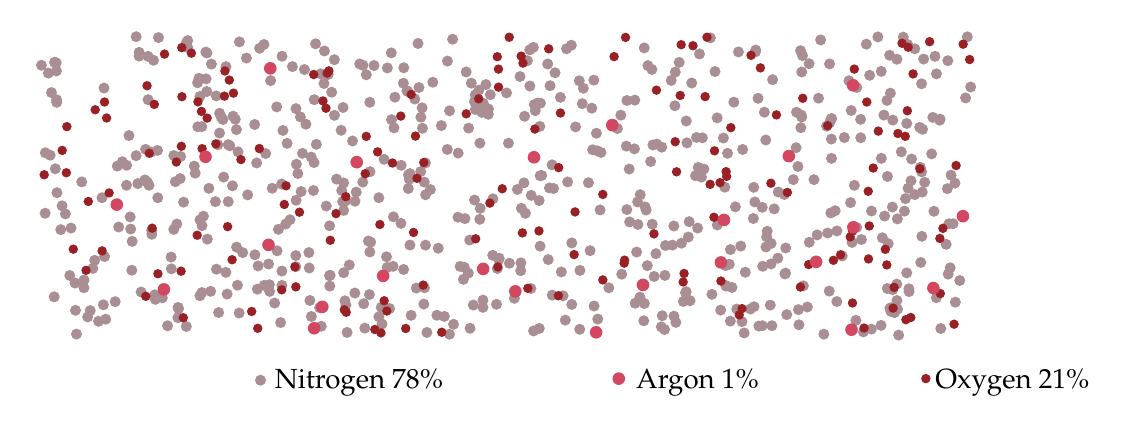
\begin{tikzpicture}
		\draw[white] (0,0) rectangle (\textwidth,4);

		\foreach \i in {1,...,624} {
				\fill[red1!60!pag] ({(\textwidth/2)+((\textwidth/2.05))*rand},2+1.9*rand) circle (0.07);
			}

		\foreach \i in {1,...,168} {
				\fill[red10!70!pag] ({(\textwidth/2)+((\textwidth/2.05))*rand},2+1.9*rand) circle (0.06);
			}
		\foreach \i in {1,...,24} {
				\fill[red5!80!pag] ({(\textwidth/2)+((\textwidth/2.05))*rand},2+1.9*rand) circle (0.08);
			}

		\fill[red1!60!pag] (2.95,-0.47)  circle (0.07);
		\node at (4.2,-0.5) {Nitrogen 78\% };

		\fill[red10!70!pag] (11.4,-0.45)  circle (0.06);
		\node at (12.5,-0.5) {Oxygen 21\% };
		\fill[red5!80!pag] (7.5,-0.45)  circle (0.08);
		\node at (8.5,-0.5) {Argon 1\% };
		% ... [Other circles with color3]
	\end{tikzpicture}
\end{center}

\section*{\LARGE\uline{Kinetic Molecular Theory of Gases}}

\begin{minipage}{4.4cm}
	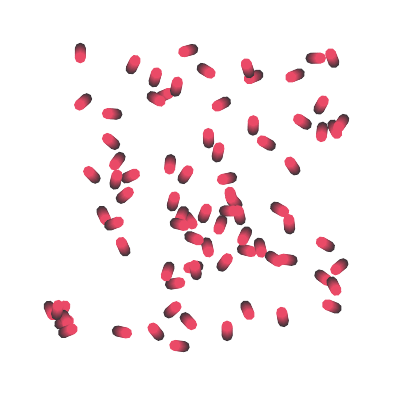
\begin{tikzpicture}
		\draw [white] (-2.15,-2.15) rectangle (2.15,2.15);
		\foreach \x in {-1.5,-1.125,...,1.5}
		\foreach \y in {-1.5,-1.125,...,1.5}
			{\pgfmathsetmacro{\myangle}{360*rnd}
				\pic[rotate=\myangle] at ({(0*\x)+1.9*rand},{(0*\y)+1.9*rand}) {balls};}
	\end{tikzpicture}
\end{minipage}
\begin{minipage}{11.8cm}
	\textbf{Ideal Gas} - To use kinetic molecular theory of gases, we need to define the definition of an ideal gas. See the following criteria.
	\begin{itemize}
		\item Many particles in random motion
		\item Negligible particle volume
		\item Collide with each other and walls
		\item No inter-particle forces
		\item Total kinetic energy is conserved
	\end{itemize}
\end{minipage}

\vspace{10pt}
\noindent\textbf{1D Pressure} - Pressure inside of a system is generated by the force exerted when a particle of the gas bounces off the one of the walls of the system. Using standard pressure and force formulas, we can derive an equation for the pressure exerted on a wall by a single particle moving in one dimension. In this formula, $u_i$ refers to the initial velocity. When it strikes the wall of area $A$, its velocity is inverted, giving us $2u_i$. \\
\begin{qq}

	\begin{center}
		$P=\frac{F}{A} \quad\quad a=\frac{\Delta u}{\Delta t} \quad\quad u=\frac{\Delta d}{\Delta t} \quad\quad F=ma \quad\quad P=\frac{ma}{A}=\frac{\frac{\Delta u}{\Delta t}}{l_\alpha\cdot\l_\gamma}=\frac{m\cdot\frac{2u_i}{2l_\beta \div u_i} }{l_\alpha\cdot\l_\gamma}=\frac{mu_i^2}{l_\alpha\cdot\l_\gamma\cdot l_\beta}=\frac{mu_1^2}{V} $
	\end{center}

\end{qq}

\pagebreak

\noindent \textbf{3D Pressure} - The equation above only applies for a singular particle moving in one dimension. If you scale the formula to account for the number of particles, and the other two dimensions, we get a new equation where $N$ refers to the number of particles, and $u^2$ refers to the average of there squared velocities. We multiply it by a third as on average, the one third of the particles are going in each dimensional direction.\\

\vspace{10pt}
\hspace{-15pt}\begin{minipage}{0.45\textwidth}

	\textbf{Average Particle Velocity} - Since the above definition relies on the average particle velocity, there are a number of ways in which we can define it. The most useful is rms, which stands for root mean square. It is equivalent to the square root of the mean squared velocity ($\sqrt{\overline{u^2}}$).
	\vspace{5pt}

	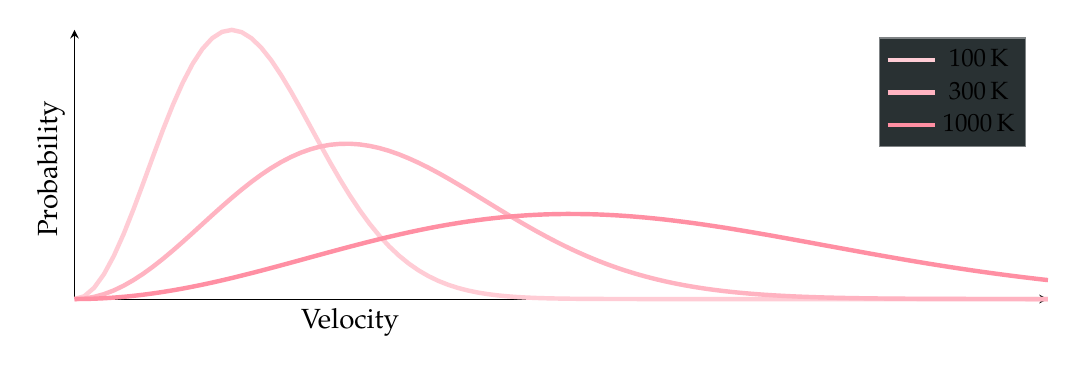
\begin{tikzpicture}[scale=1]
		\begin{axis}[
				axis lines=middle,
				xlabel=,
				ylabel={},
				legend style={
						fill=pag, draw=pag!60, % Red background with black border
						font=\small, % Smaller font size
						inner sep=2pt, % Inner spacing (padding around the text)
						outer sep=1pt  % Outer spacing (margin around the border)
					},
				domain=0:8000,
				xtick=\empty,
				ytick=\empty,
				grid=both,
				grid style={line width=.1pt, draw=gray!10},
				major grid style={line width=.2pt,draw=gray!50},
				minor tick num=5,
				width=1.15*\textwidth,
				height=5cm,
				clip=false,
				ticklabel style={font=\tiny,fill=white},
				xlabel style={at={(ticklabel* cs:1)},anchor=north west},
				ylabel style={at={(ticklabel* cs:1)},anchor=south west},
			]
			% Function f(x) = 1/x

			\addplot[color=red1,ultra thick,samples=100]{\maxwellboltzmann{100}};

			\addplot[color=red2,ultra thick,samples=100]{\maxwellboltzmann{300}};

			\addplot[color=red3,ultra thick,samples=100]{\maxwellboltzmann{1000}};
			\legend{\SI{100}{\kelvin}, \SI{300}{\kelvin}, \SI{1000}{\kelvin}}
		\end{axis}
		\node at (3.5,-0.3) {Velocity};
		\node[rotate=90] at (-0.3,1.65) {Probability};

	\end{tikzpicture}
\end{minipage}
\hspace{5pt}\begin{minipage}{0.55\textwidth}
	\tdplotsetmaincoords{70}{155}
	\vspace{5pt}
	\begin{tikzpicture}
		[tdplot_main_coords,
			grid/.style={very thin,gray},
			axis/.style={->,blue,thick},
			cube/.style={opacity=.5,very thick,},scale=2.15]
		% draw a grid in the x-y plane
		\foreach \x in {-0.5,0,...,2.5}
		\foreach \y in {-0.5,0,...,2.5}
			{
				\draw[grid] (\x,-0.5) -- (\x,2.5);
				\draw[grid] (-0.5,\y) -- (2.5,\y);
			}
		% draw the bottom of the cube
		\draw[cube,fill=pag!80] (0,0,0) -- (0,2,0) -- (2,2,0) -- (2,0,0) -- cycle;

		% draw the back-right of the cube
		\draw[cube,fill=pag!80] (0,0,0) -- (0,2,0) -- (0,2,2) -- (0,0,2) -- cycle;

		% draw the back-left of the cube
		\draw[cube,fill=pag!80] (0,0,0) -- (2,0,0) -- (2,0,2) -- (0,0,2) -- cycle;

		\foreach \z in {0,0.125,...,1}
		\foreach \x in {0,0.125,...,1}
		\foreach \y in {0,0.125,...,1}{\pgfmathsetmacro{\myangle}{360*rnd}
				\pic[rotate =\myangle] at ({(0*\x)+1+0.99*rand},{(0*\y)+1+0.99*rand},{(0*\z)+1+0.99*rand}) {threedballs}; }
		% draw the axes

		% draw the front-right of the cube
		\draw[cube] (2,0,0) -- (2,2,0) -- (2,2,2) -- (2,0,2) -- cycle;

		% draw the front-left of the cube
		\draw[cube] (0,2,0) -- (2,2,0) -- (2,2,2) -- (0,2,2) -- cycle;

		% draw the top of the cube
		\draw[cube] (0,0,2) -- (0,2,2) -- (2,2,2) -- (2,0,2) -- cycle;

	\end{tikzpicture}

\end{minipage}

\vspace{10pt}
\begin{qq}

	\begin{center}
		$p=\frac{1}{3}\cdot\frac{M\overline{u^2}}{V} \qquad \overline{u^2}=\frac{1}{N}\left(u_1^2+u_2^2\cdots u_n^2\right)$\\
		\vspace{5pt}
		$M=\text{Molar Mass}=N_Am \qquad N_A=\text{Avagadro's No.}\qquad m=\text{Mass of 1 Particle}$
	\end{center}

\end{qq}
\vspace{10pt}

\noindent\textbf{Deriving Average Velocity} - Combined with ideal gas law, we get two formulas for pressure. Subsequently, we can derive a formula to calculate the rms velocity by setting the two pressure formulas equal to each other. We also assume that there is only one mol of gas present.
\begin{qq}

	\begin{center}
		$\frac{1}{3}\cdot\frac{m\overline{u^2}}{V}=\frac{nRT}{V} \longrightarrow \overline{u^2}=\frac{3RT}{M}\longrightarrow u_{rms}=\sqrt{\overline{u^2}}=\sqrt{\frac{3RT}{M}} \qquad R=8.314\frac{j}{mol\cdot K}$
	\end{center}

\end{qq}

\vspace{3pt}
\noindent Using this equation, we can see that the higher the temperature, the greater the average speed of the gas particles. Lighter gas particles will also increase this value. It's also important to note that whatever the $u_{rms}$ may be for some gas is not representative of the speed that particles move across the system, as the gas particles will bump into each other as they travel.\\
\\
\textbf{Temperature} - Temperature is a measure of kinetic energy. To relate temperature in our formulas, we can use all the equations above and the formula for kinetic energy. Its it important to note that all $E_k$ refer to the \textbf{average kinetic energy} of a particle in the system. We end up finding that the average kinetic energy of a particle is proportional to the temperature. Temperature for a one-particle system would be meaningless. A temperature of zero would mean no kinetic energy whatsoever, which is impossible.
\begin{qq}

	\begin{center}
		$E_k=\frac{1}{2}mu^2\longrightarrow E_k=N_A\frac{1}{2}m\overline{u^2}\longrightarrow \overline{u^2}=\frac{2E_k}{N_Am}$\\
		\vspace{5pt}
		$P=\frac{1}{3}\frac{N_Am}{V}\cdot\overline{u^2}\longrightarrow P=\frac{1}{3}\frac{N_Am}{V}\cdot\frac{2E_k}{N_A}=\frac{2}{3}\cdot\frac{E_k}{V}$\\
		\vspace{5pt}
		$P=\frac{2}{3}\cdot\frac{E_k}{V}=\frac{uRT}{V}\longrightarrow E_k=\frac{3}{2}RT$\\
		\vspace{5pt}
		$\therefore \quad E_{k(avg)}\propto T$
	\end{center}

\end{qq}
\pagebreak

\noindent\textbf{Temperatures Effect} - Based on all that we have talked about, we can infer the effect of temperature on things like volume or pressure. Below, the temperature is increased and thus the pressure. To maintain the same pressure, the volume of the system must expand
\begin{qq}

	\begin{center}

		\tdplotsetmaincoords{70}{165}
		\begin{tikzpicture}
			[tdplot_main_coords,
				grid/.style={very thin,gray},
				axis/.style={->,blue,thick},
				cube/.style={opacity=.5,very thick,},scale=1]
			% draw a grid in the x-y plane
			\foreach \x in {-0.5,0,...,2.5}
			\foreach \y in {-0.5,0,...,2.5}
				{
					\draw[grid] (\x,-0.5) -- (\x,2.5);
					\draw[grid] (-0.5,\y) -- (2.5,\y);
				}
			% draw the bottom of the cube
			\draw[cube,fill=pag!80] (0,0,0) -- (0,2,0) -- (2,2,0) -- (2,0,0) -- cycle;

			% draw the back-right of the cube
			\draw[cube,fill=pag!80] (0,0,0) -- (0,2,0) -- (0,2,2) -- (0,0,2) -- cycle;

			% draw the back-left of the cube
			\draw[cube,fill=pag!80] (0,0,0) -- (2,0,0) -- (2,0,2) -- (0,0,2) -- cycle;

			\foreach \z in {0,0.2,...,1}
			\foreach \x in {0,0.2,...,1}
			\foreach \y in {0,0.2,...,1}{\pgfmathsetmacro{\myangle}{360*rnd}
					\pic[rotate =\myangle] at ({(0*\x)+1+0.99*rand},{(0*\y)+1+0.99*rand},{(0*\z)+1+0.99*rand}) {threedballs}; }
			% draw the axes

			% draw the front-right of the cube
			\draw[cube] (2,0,0) -- (2,2,0) -- (2,2,2) -- (2,0,2) -- cycle;

			% draw the front-left of the cube
			\draw[cube] (0,2,0) -- (2,2,0) -- (2,2,2) -- (0,2,2) -- cycle;

			% draw the top of the cube
			\draw[cube] (0,0,2) -- (0,2,2) -- (2,2,2) -- (2,0,2) -- cycle;

		\end{tikzpicture}
		\tdplotsetmaincoords{70}{165}
		\begin{tikzpicture}
			[tdplot_main_coords,
				grid/.style={very thin,gray},
				axis/.style={->,blue,thick},
				cube/.style={opacity=.5,very thick,},scale=1]
			% draw a grid in the x-y plane
			\foreach \x in {-0.5,0,...,2.5}
			\foreach \y in {-0.5,0,...,2.5}
				{
					\draw[grid] (\x,-0.5) -- (\x,2.5);
					\draw[grid] (-0.5,\y) -- (2.5,\y);
				}
			% draw the bottom of the cube
			\draw[cube,fill=pag!80] (0,0,0) -- (0,2,0) -- (2,2,0) -- (2,0,0) -- cycle;

			% draw the back-right of the cube
			\draw[cube,fill=pag!80] (0,0,0) -- (0,2,0) -- (0,2,2) -- (0,0,2) -- cycle;

			% draw the back-left of the cube
			\draw[cube,fill=pag!80] (0,0,0) -- (2,0,0) -- (2,0,2) -- (0,0,2) -- cycle;

			\foreach \z in {0,0.2,...,1}
			\foreach \x in {0,0.2,...,1}
			\foreach \y in {0,0.2,...,1}{\pgfmathsetmacro{\myangle}{360*rnd}
					\pic[rotate =\myangle] at ({(0*\x)+1+0.925	*rand},{(0*\y)+1+0.925*rand},{(0*\z)+1+0.99*rand}) {threedballstwo}; }
			% draw the axes

			% draw the front-right of the cube
			\draw[cube] (2,0,0) -- (2,2,0) -- (2,2,2) -- (2,0,2) -- cycle;

			% draw the front-left of the cube
			\draw[cube] (0,2,0) -- (2,2,0) -- (2,2,2) -- (0,2,2) -- cycle;

			% draw the top of the cube
			\draw[cube] (0,0,2) -- (0,2,2) -- (2,2,2) -- (2,0,2) -- cycle;

		\end{tikzpicture}
		\tdplotsetmaincoords{70}{165}\hspace{10pt}\begin{tikzpicture}
			[tdplot_main_coords,
				grid/.style={very thin,gray},
				axis/.style={->,blue,thick},
				cube/.style={opacity=.5,very thick,},scale=1]
			% draw a grid in the x-y plane
			\foreach \x in {-0.5,0,...,3.5}
			\foreach \y in {-0.5,0,...,3.5}
				{
					\draw[grid] (\x,-0.5) -- (\x,3.5);
					\draw[grid] (-0.5,\y) -- (3.5,\y);
				}
			% draw the bottom of the cube
			\draw[cube,fill=pag!80] (0,0,0) -- (0,3,0) -- (3,3,0) -- (3,0,0) -- cycle;

			% draw the back-right of the cube
			\draw[cube,fill=pag!80] (0,0,0) -- (0,3,0) -- (0,3,3) -- (0,0,3) -- cycle;

			% draw the back-left of the cube
			\draw[cube,fill=pag!80] (0,0,0) -- (3,0,0) -- (3,0,3) -- (0,0,3) -- cycle;

			\foreach \z in {0,0.2,...,1}
			\foreach \x in {0,0.2,...,1}
			\foreach \y in {0,0.2,...,1}{\pgfmathsetmacro{\myangle}{360*rnd}
					\pic[rotate =\myangle] at ({(0*\x)+1.5+1.49*rand},{(0*\y)+1.5+1.49*rand},{(0*\z)+1.5+1.49*rand}) {threedballs}; }
			% draw the axes

			% draw the front-right of the cube
			\draw[cube] (3,0,0) -- (3,3,0) -- (3,3,3) -- (3,0,3) -- cycle;

			% draw the front-left of the cube
			\draw[cube] (0,3,0) -- (3,3,0) -- (3,3,3) -- (0,3,3) -- cycle;

			% draw the top of the cube
			\draw[cube] (0,0,3) -- (0,3,3) -- (3,3,3) -- (3,0,3) -- cycle;

		\end{tikzpicture}
	\end{center}

\end{qq}

\vspace{10pt}
\noindent\textbf{Real Gases} - In real life, gases contained in some system will never completely obey the ideal gas law. We can define the deviation from the standard behavior of a ideal gas as compressibility. For an ideal gas, $\frac{pV}{nRT}$ will equal 1. We can denote this as $Z$. In a real gas, $Z$ will never be 1. More ideal gas behavior occurs when pressure is low and temperature is high. When the temperature is low, the effect of particle-particle collisions has a greater influence as the overall time between hitting walls of the system is increased.\\
\\
\textbf{Pressure Deviation} - When changing the pressure, there are two cases where the pressure will cause a deviation in compressibility from the ideal ratio.\\
\begin{itemize}
	\item \textbf{Inter-Particle Forces} - When you begin to decrease the pressure, the inter particle forces begin to increase as the particles are forced closer together. The inter-particle forces are primarily responsible from ideal deviation, and $Z$ is less then 1.
	\item \textbf{Particle Volume} - When the pressure is increased drastically, the volume of the particles will begin to outweigh the volume of the container. In turn, the the main factor for the deviation from an ideal gas is volume, and $Z$ is greater then 1.
\end{itemize}

\tdplotsetmaincoords{70}{165}
\begin{qq}

	\begin{center}
		\begin{minipage}{\textwidth}
			\hspace{5pt}\begin{tikzpicture}
				[tdplot_main_coords,
					grid/.style={very thin,gray},
					axis/.style={->,blue,thick},
					cube/.style={opacity=.5,very thick,},scale=1]
				% draw a grid in the x-y plane
				\foreach \x in {-0.5,0,...,3.5}
				\foreach \y in {-0.5,0,...,3.5}
					{
						\draw[grid] (\x,-0.5) -- (\x,3.5);
						\draw[grid] (-0.5,\y) -- (3.5,\y);
					}
				% draw the bottom of the cube
				\draw[cube,fill=pag!80] (0,0,0) -- (0,3,0) -- (3,3,0) -- (3,0,0) -- cycle;

				% draw the back-right of the cube
				\draw[cube,fill=pag!80] (0,0,0) -- (0,3,0) -- (0,3,3) -- (0,0,3) -- cycle;

				% draw the back-left of the cube
				\draw[cube,fill=pag!80] (0,0,0) -- (3,0,0) -- (3,0,3) -- (0,0,3) -- cycle;

				\foreach \z in {0,0.15,...,1}
				\foreach \x in {0,0.15,...,1}
				\foreach \y in {0,0.15,...,1}{\pgfmathsetmacro{\myangle}{360*rnd}
						\pic[rotate =\myangle] at ({(0*\x)+1.5+1.49*rand},{(0*\y)+1.5+1.49*rand},{(0*\z)+1.5+1.49*rand}) {threedballs}; }
				% draw the axes

				% draw the front-right of the cube
				\draw[cube] (3,0,0) -- (3,3,0) -- (3,3,3) -- (3,0,3) -- cycle;

				% draw the front-left of the cube
				\draw[cube] (0,3,0) -- (3,3,0) -- (3,3,3) -- (0,3,3) -- cycle;

				% draw the top of the cube
				\draw[cube] (0,0,3) -- (0,3,3) -- (3,3,3) -- (3,0,3) -- cycle;

			\end{tikzpicture}
			\begin{tikzpicture}
				[tdplot_main_coords,
					grid/.style={very thin,gray},
					axis/.style={->,blue,thick},
					cube/.style={opacity=.5,very thick,},scale=1]
				% draw a grid in the x-y plane
				\foreach \x in {-0.5,0,...,3.5}
				\foreach \y in {-0.5,0,...,3.5}
					{
						\draw[grid] (\x,-0.5) -- (\x,3.5);
						\draw[grid] (-0.5,\y) -- (3.5,\y);
					}
				% draw the bottom of the cube
				\draw[cube,fill=pag!80] (0,0,0) -- (0,3,0) -- (3,3,0) -- (3,0,0) -- cycle;

				% draw the back-right of the cube
				\draw[cube,fill=pag!80] (0,0,0) -- (0,3,0) -- (0,3,2) -- (0,0,2) -- cycle;

				% draw the back-left of the cube
				\draw[cube,fill=pag!80] (0,0,0) -- (3,0,0) -- (3,0,2) -- (0,0,2) -- cycle;

				\foreach \z in {0,0.1333,...,1}
				\foreach \x in {0,0.1333,...,1}
				\foreach \y in {0,0.11333,...,1}{\pgfmathsetmacro{\myangle}{360*rnd}
						\pic[rotate =\myangle] at ({(0*\x)+1.5+1.49*rand},{(0*\y)+1.5+1.49*rand},{(0*\z)+1+0.99*rand}) {threedballs}; }
				% draw the axes

				% draw the front-right of the cube
				% draw the front-right of the cube
				\draw[cube] (3,0,0) -- (3,3,0) -- (3,3,2) -- (3,0,2) -- cycle;

				% draw the front-left of the cube
				\draw[cube] (0,3,0) -- (3,3,0) -- (3,3,2) -- (0,3,2) -- cycle;

				% draw the top of the cube
				\draw[cube] (0,0,2) -- (0,3,2) -- (3,3,2) -- (3,0,2) -- cycle;

			\end{tikzpicture}
			\begin{tikzpicture}
				[tdplot_main_coords,
					grid/.style={very thin,gray},
					axis/.style={->,blue,thick},
					cube/.style={opacity=.5,very thick,},scale=1]
				% draw a grid in the x-y plane
				\foreach \x in {-0.5,0,...,3.5}
				\foreach \y in {-0.5,0,...,3.5}
					{
						\draw[grid] (\x,-0.5) -- (\x,3.5);
						\draw[grid] (-0.5,\y) -- (3.5,\y);
					}
				% draw the bottom of the cube
				\draw[cube,fill=pag!80] (0,0,0) -- (0,3,0) -- (3,3,0) -- (3,0,0) -- cycle;

				% draw the back-right of the cube
				\draw[cube,fill=pag!80] (0,0,0) -- (0,3,0) -- (0,3,1) -- (0,0,1) -- cycle;

				% draw the back-left of the cube
				\draw[cube,fill=pag!80] (0,0,0) -- (3,0,0) -- (3,0,1) -- (0,0,1) -- cycle;

				\foreach \z in {0,0.1,...,1}
				\foreach \x in {0,0.1,...,1}
				\foreach \y in {0,0.1,...,1}{\pgfmathsetmacro{\myangle}{360*rnd}
						\pic[rotate =\myangle] at ({(0*\x)+1.5+1.49*rand},{(0*\y)+1.5+1.49*rand},{(0*\z)+0.5+0.49*rand}) {threedballs}; }
				% draw the axes

				% draw the front-right of the cube
				% draw the front-right of the cube
				\draw[cube] (3,0,0) -- (3,3,0) -- (3,3,1) -- (3,0,1) -- cycle;

				% draw the front-left of the cube
				\draw[cube] (0,3,0) -- (3,3,0) -- (3,3,1) -- (0,3,1) -- cycle;

				% draw the top of the cube
				\draw[cube] (0,0,1) -- (0,3,1) -- (3,3,1) -- (3,0,1) -- cycle;

			\end{tikzpicture}
		\end{minipage}
	\end{center}
	$\qquad\qquad\qquad\:\: Z=1 \qquad\qquad\qquad\qquad\qquad\qquad   Z<1 \qquad\qquad\qquad\qquad\qquad\qquad Z>1$
\end{qq}
\vspace{10pt}
\noindent\textbf{Van der Waals Equation} - If we apply corrections accounting for these deviations, we get the van der Waals equation, which uses $a$ and $b$. These two variables change between gases.
\begin{qq}

	\begin{center}
		$P=\frac{nRT}{V-nb}-a\left(\frac{n}{v}\right)^2 \quad\quad \lor \qquad \left(P+\frac{u^2a}{V^2}\right)\left(V-ub\right)=RT$
	\end{center}

\end{qq}

\pagebreak

\newcommand{\Tstrut}{\rule{0pt}{3.1ex}}         % Top strut
\newcommand{\Bstrut}{\rule[-2ex]{0pt}{0pt}}   % Bottom strut
\newcommand{\TBstrut}{\Tstrut\Bstrut}            % Top and Bottom strut

\noindent In van der Waals equation, $a$ represents the magnitude of attractive forces between the particles, and $b$ represents the effective volume occupied by the gas molecules. Below is a table of the $a$ and $b$ values for various gases.

\begin{center}
	\begin{tabular}{ccccccc}
		\hline
		\textbf{Gas}                                                  & \textcolor{pag!40}{He} & \textcolor{pag!40}{Ar} & \textcolor{pag!40}{H$_2$} & \textcolor{pag!40}{O$_2$} & \textcolor{pag!40}{CO$_2$} & \textcolor{pag!40}{Cl$_2$} \\
		\hline
		$a\:\: \left(\frac{\text{atm}\cdot L^2}{\text{mol}^2}\right)$ & 0.034                  & 1.35                   & 0.244                     & 1.36                      & 3.59                       & 6.49 \TBstrut              \\
		$b\:\: \left(\frac{L}{\text{mol}}\right)$                     & 0.0237                 & 0.0322                 & 0.0266                    & 0.0318                    & 0.0427                     & 0.0562 \TBstrut            \\
		\hline
	\end{tabular}
\end{center}

\section*{\LARGE\uline{Phase Change}}
Everyone knows the 3 standard states of matter. Usually, temperature is the sole factor dictating the state that some matter in a particular system is in. When talking about gas laws however, when the pressure is increased to extreme levels, the gas in some system will eventually turn to a liquid, and with even higher levels, a solid. Its important to remember the two factors that effect kinetic energy in a system (or phase change) are temperature and pressure.
\vspace{20pt}

\begin{minipage}{25cm}
	\begin{center}
		\tdplotsetmaincoords{70}{165}
		\hspace{-9.2cm}	\begin{tikzpicture}
			[tdplot_main_coords,
				grid/.style={very thin,gray},
				axis/.style={->,blue,thick},
				cube/.style={opacity=.5,very thick,},scale=2]
			% draw a grid in the x-y plane
			\foreach \x in {1,1.5,...,3.5}
			\foreach \y in {1,1.5,...,3.5}
				{
					\draw[grid] (\x,1) -- (\x,3.5);
					\draw[grid] (1,\y) -- (3.5,\y);
				}
			% draw the bottom of the cube
			\draw[cube,fill=pag!80,thin] (1.5,1.5,0) -- (1.5,3,0) -- (3,3,0) -- (3,1.5,0) -- cycle;

			% draw the back-right of the cube
			\draw[cube,fill=pag!80,thin] (1.5,1.5,0) -- (1.5,3,0) -- (1.5,3,2) -- (1.5,1.5,2) -- cycle;

			% draw the back-left of the cube
			\draw[cube,fill=pag!80,thin] (1.5,1.5,0) -- (3,1.5,0) -- (3,1.5,2) -- (1.5,1.5,2) -- cycle;

			\foreach \z in {0,0.2,...,1.85}
			\foreach \x in {1.6,1.8,...,2.9}
			\foreach \y in {1.6,1.8,...,2.9}{\pgfmathsetmacro{\myangle}{360*rnd}
					\pic at ({\x+(0.05*rand)},{\y+(0.1*rand)},{0.1+\z+(0.1*rand/2)}) {threedballsthree}; }
			% draw the axes

			% draw the front-right of the cube
			% draw the front-right of the cube
			\draw[cube,thin] (3,1.5,0) -- (3,3,0) -- (3,3,2) -- (3,1.5,2) -- cycle;

			% draw the front-left of the cube
			\draw[cube,thin] (1.5,3,0) -- (3,3,0) -- (3,3,2) -- (1.5,3,2) -- cycle;

			% draw the top of the cube
			\draw[cube,thin] (1.5,1.5,2) -- (1.5,3,2) -- (3,3,2) -- (3,1.5,2) -- cycle;

		\end{tikzpicture}
		\newcommand{\randomnessfactor}{0.05}
		\hspace{5pt}\begin{tikzpicture}
			[tdplot_main_coords,
				grid/.style={very thin,gray},
				axis/.style={->,blue,thick},
				cube/.style={opacity=.5,very thick,},scale=2]
			% draw a grid in the x-y plane
			\foreach \x in {1,1.5,...,3.5}
			\foreach \y in {1,1.5,...,3.5}
				{
					\draw[grid] (\x,1) -- (\x,3.5);
					\draw[grid] (1,\y) -- (3.5,\y);
				}
			% draw the bottom of the cube
			\draw[cube,fill=pag!80,thin] (1.5,1.5,0) -- (1.5,3,0) -- (3,3,0) -- (3,1.5,0) -- cycle;

			% draw the back-right of the cube
			\draw[cube,fill=pag!80,thin] (1.5,1.5,0) -- (1.5,3,0) -- (1.5,3,0.5) -- (1.5,1.5,0.5) -- cycle;

			% draw the back-left of the cube
			\draw[cube,fill=pag!80,thin] (1.5,1.5,0) -- (3,1.5,0) -- (3,1.5,0.5) -- (1.5,1.5,0.5) -- cycle;

			\foreach \z in {0,0.1,...,0.45}
			\foreach \x in {1.6,1.65,...,2.9}
			\foreach \y in {1.6,1.65,...,2.9}{\pgfmathsetmacro{\myangle}{360*rnd}
					\pic at ({\x+(\randomnessfactor*rand)},{\y+(\randomnessfactor*rand)},{0.05+\z+(0.05*rand/2)}) {threedballsthree}; }

			\foreach \z in {0,0.025,...,0.5}
			\foreach \x in {1.6,1.65,...,2.9}
			\foreach \y in {2.9}{\pgfmathsetmacro{\myangle}{360*rnd}
					\pic at ({\x+(\randomnessfactor*rand)},{\y},{0.05+\z+(0.05*rand)}) {threedballsthree}; }
			% draw the axes
			\foreach \z in {0,0.025,...,0.45}
			\foreach \x in {2.9}
			\foreach \y in {1.6,1.7,...,2.9}{\pgfmathsetmacro{\myangle}{360*rnd}
					\pic at ({\x},{\y+(\randomnessfactor*rand)},{0.05+\z+(0.05*rand)}) {threedballsthree}; }

			\foreach \z in {0.5}
			\foreach \x in {1.6,1.65,...,2.9}
			\foreach \y in {1.6,1.65,...,2.9}{\pgfmathsetmacro{\myangle}{360*rnd}
					\pic at ({\x+(\randomnessfactor*rand)},{\y+(\randomnessfactor*rand)},{\z}) {threedballsthree}; }

			% draw the front-right of the cube
			\draw[cube,thin] (3,1.5,0) -- (3,3,0) -- (3,3,0.5) -- (3,1.5,0.5) -- cycle;

			% draw the front-left of the cube
			\draw[cube,thin] (1.5,3,0) -- (3,3,0) -- (3,3,0.5) -- (1.5,3,0.5) -- cycle;

			% draw the top of the cube
			\draw[cube,thin] (1.5,1.5,0.5) -- (1.5,3,0.5) -- (3,3,0.5) -- (3,1.5,0.5) -- cycle;

		\end{tikzpicture}
		\hspace{5pt}\begin{tikzpicture}
			[tdplot_main_coords,
				grid/.style={very thin,gray},
				axis/.style={->,blue,thick},
				cube/.style={opacity=.5,very thick,},scale=2]
			% draw a grid in the x-y plane
			\foreach \x in {1,1.5,...,3.5}
			\foreach \y in {1,1.5,...,3.5}
				{
					\draw[grid] (\x,1) -- (\x,3.5);
					\draw[grid] (1,\y) -- (3.5,\y);
				}
			% draw the bottom of the cube
			\draw[cube,fill=pag!80,thin] (1.5,1.5,0) -- (1.5,3,0) -- (3,3,0) -- (3,1.5,0) -- cycle;

			% draw the back-right of the cube
			\draw[cube,fill=pag!80,thin] (1.5,1.5,0) -- (1.5,3,0) -- (1.5,3,0.25) -- (1.5,1.5,0.25) -- cycle;

			% draw the back-left of the cube
			\draw[cube,fill=pag!80,thin] (1.5,1.5,0) -- (3,1.5,0) -- (3,1.5,0.25) -- (1.5,1.5,0.25) -- cycle;

			\foreach \z in {0,0.05,...,0.2}
			\foreach \x in {1.56,1.61,...,2.99}
			\foreach \y in {1.56,1.61,...,2.99}{\pgfmathsetmacro{\myangle}{360*rnd}
					\pic at ({\x},{\y},{0.05+\z}) {threedballsthree}; }

			% draw the front-right of the cube
			\draw[cube,thin] (3,1.5,0) -- (3,3,0) -- (3,3,0.25) -- (3,1.5,0.25) -- cycle;

			% draw the front-left of the cube
			\draw[cube,thin] (1.5,3,0) -- (3,3,0) -- (3,3,0.25) -- (1.5,3,0.25) -- cycle;

			% draw the top of the cube
			\draw[cube,thin] (1.5,1.5,0.25) -- (1.5,3,0.25) -- (3,3,0.25) -- (3,1.5,0.25) -- cycle;

		\end{tikzpicture}
	\end{center}
\end{minipage}

\vspace{25pt}
\noindent\textbf{Water} - For water specifically, hydrogen bonding occurs, where the hydrogen on each end of the water molecule begin to form intermolecular bonds. As the pressure increases, or temperature decreases, the relative distance between these molecules is decreased, so phase change occurs, and these hydrogen bonds form a crystalline structure.

\vspace{10pt}
\begin{minipage}{20cm}
	$\qquad\:\:\underline{\textbf{\large Gas}} \qquad\qquad\qquad\qquad\qquad\qquad\qquad\qquad\underline{\textbf{\large Liquid}}\qquad\qquad\qquad\qquad\qquad\qquad\qquad\qquad\underline{\textbf{\large Solid}}$
	\vspace{3pt}

	\hspace{-26pt}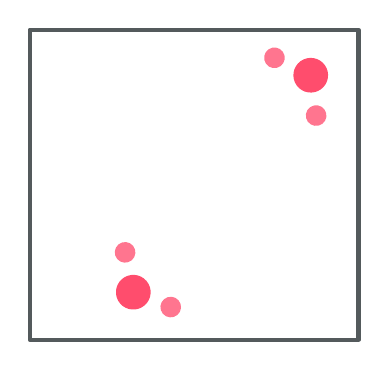
\begin{tikzpicture}[y=1cm, x=1cm, scale=0.75, inner sep=0pt, outer sep=0pt]

		\begin{scope}[shift={(-1.3062, 10.8309)}]

			\path[draw=pag!80,line join=round,line width=0.0521cm,miter limit=4.0] (12.8213, -5.572) rectangle (18.3878, -10.8199);

			\begin{scope}[cm={ -0.5125,0.6143,-0.6143,-0.5125,(12.0042, -19.8013)}]
				\path[draw=white,line cap=butt,line join=miter,line width=0.1323cm,miter limit=4.0] (7.3092, -10.2923) -- (6.5625, -10.6981);

				\path[draw=white,line cap=butt,line join=miter,line width=0.1323cm,miter limit=4.0] (8.0721, -10.7144) -- (7.3254, -10.2923);

				\path[fill=cff758f,cm={ 0.223,-0.0,-0.0,0.223,(5.4926, -10.1251)}] (5.8738, -2.6207).. controls (5.8738, -3.1614) and (5.4355, -3.5997) .. (4.8948, -3.5997).. controls (4.3541, -3.5997) and (3.9158, -3.1614) .. (3.9158, -2.6207).. controls (3.9158, -2.0801) and (4.3541, -1.6418) .. (4.8948, -1.6418).. controls (5.4355, -1.6418) and (5.8738, -2.0801) .. (5.8738, -2.6207) -- cycle;

				\path[fill=cff4d6d,cm={ 0.375,-0.0,-0.0,0.375,(5.4975, -9.3198)}] (5.8738, -2.6207).. controls (5.8738, -3.1614) and (5.4355, -3.5997) .. (4.8948, -3.5997).. controls (4.3541, -3.5997) and (3.9158, -3.1614) .. (3.9158, -2.6207).. controls (3.9158, -2.0801) and (4.3541, -1.6418) .. (4.8948, -1.6418).. controls (5.4355, -1.6418) and (5.8738, -2.0801) .. (5.8738, -2.6207) -- cycle;

				\path[fill=cff758f,cm={ 0.223,-0.0,-0.0,0.223,(7.0007, -10.1251)}] (5.8738, -2.6207).. controls (5.8738, -3.1614) and (5.4355, -3.5997) .. (4.8948, -3.5997).. controls (4.3541, -3.5997) and (3.9158, -3.1614) .. (3.9158, -2.6207).. controls (3.9158, -2.0801) and (4.3541, -1.6418) .. (4.8948, -1.6418).. controls (5.4355, -1.6418) and (5.8738, -2.0801) .. (5.8738, -2.6207) -- cycle;

			\end{scope}
			\begin{scope}[cm={ 0.4682,-0.6487,0.6487,0.4682,(20.8292, 3.2378)}]
				\path[draw=white,line cap=butt,line join=miter,line width=0.1323cm,miter limit=4.0] (7.3092, -10.2923) -- (6.5625, -10.6981);

				\path[draw=white,line cap=butt,line join=miter,line width=0.1323cm,miter limit=4.0] (8.0721, -10.7144) -- (7.3254, -10.2923);

				\path[fill=cff758f,cm={ 0.223,-0.0,-0.0,0.223,(5.4926, -10.1251)}] (5.8738, -2.6207).. controls (5.8738, -3.1614) and (5.4355, -3.5997) .. (4.8948, -3.5997).. controls (4.3541, -3.5997) and (3.9158, -3.1614) .. (3.9158, -2.6207).. controls (3.9158, -2.0801) and (4.3541, -1.6418) .. (4.8948, -1.6418).. controls (5.4355, -1.6418) and (5.8738, -2.0801) .. (5.8738, -2.6207) -- cycle;

				\path[fill=cff4d6d,line width=0.3528cm,cm={ 0.375,-0.0,-0.0,0.375,(5.4975, -9.3198)}] (5.8738, -2.6207).. controls (5.8738, -3.1614) and (5.4355, -3.5997) .. (4.8948, -3.5997).. controls (4.3541, -3.5997) and (3.9158, -3.1614) .. (3.9158, -2.6207).. controls (3.9158, -2.0801) and (4.3541, -1.6418) .. (4.8948, -1.6418).. controls (5.4355, -1.6418) and (5.8738, -2.0801) .. (5.8738, -2.6207) -- cycle;

				\path[fill=cff758f,cm={ 0.223,-0.0,-0.0,0.223,(7.0007, -10.1251)}] (5.8738, -2.6207).. controls (5.8738, -3.1614) and (5.4355, -3.5997) .. (4.8948, -3.5997).. controls (4.3541, -3.5997) and (3.9158, -3.1614) .. (3.9158, -2.6207).. controls (3.9158, -2.0801) and (4.3541, -1.6418) .. (4.8948, -1.6418).. controls (5.4355, -1.6418) and (5.8738, -2.0801) .. (5.8738, -2.6207) -- cycle;

			\end{scope}

			% 

			\path[draw=pag!80,line join=round,line width=0.0221cm,miter limit=4.0] (12.8213, -5.572) rectangle (18.3878, -10.8199);
		\end{scope}

	\end{tikzpicture}
	\hspace{68pt}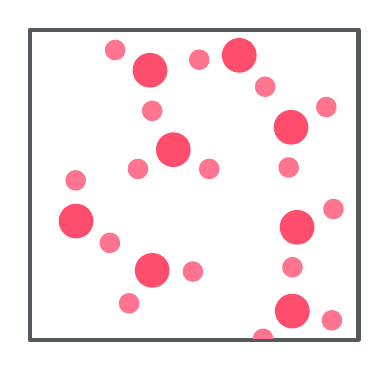
\begin{tikzpicture}[y=1cm, x=1cm, scale=0.75, inner sep=0pt, outer sep=0pt]
		\begin{scope}[shift={(-1.3062, 10.8309)}]

			\path[draw=pag!80, line join=round,line width=0.0521cm,miter limit=4.0] (7.0693, -5.572) rectangle (12.6358, -10.8199);

			% 
			\begin{scope}
				\clip (7.0693, -5.572) rectangle (12.6358, -10.8199);
				\begin{scope}[cm={ 0.7727,0.2073,-0.2073,0.7727,(3.7133, -3.895)}]
					\path[draw=white,line cap=butt,line join=miter,line width=0.1323cm,miter limit=4.0] (7.3092, -10.2923) -- (6.5625, -10.6981);

					\path[draw=white,line cap=butt,line join=miter,line width=0.1323cm,miter limit=4.0] (8.0721, -10.7144) -- (7.3254, -10.2923);

					\path[fill=cff758f,cm={ 0.223,-0.0,-0.0,0.223,(5.4926, -10.1251)}] (5.8738, -2.6207).. controls (5.8738, -3.1614) and (5.4355, -3.5997) .. (4.8948, -3.5997).. controls (4.3541, -3.5997) and (3.9158, -3.1614) .. (3.9158, -2.6207).. controls (3.9158, -2.0801) and (4.3541, -1.6418) .. (4.8948, -1.6418).. controls (5.4355, -1.6418) and (5.8738, -2.0801) .. (5.8738, -2.6207) -- cycle;

					\path[fill=cff4d6d,cm={ 0.375,-0.0,-0.0,0.375,(5.4975, -9.3198)}] (5.8738, -2.6207).. controls (5.8738, -3.1614) and (5.4355, -3.5997) .. (4.8948, -3.5997).. controls (4.3541, -3.5997) and (3.9158, -3.1614) .. (3.9158, -2.6207).. controls (3.9158, -2.0801) and (4.3541, -1.6418) .. (4.8948, -1.6418).. controls (5.4355, -1.6418) and (5.8738, -2.0801) .. (5.8738, -2.6207) -- cycle;

					\path[fill=cff758f,cm={ 0.223,-0.0,-0.0,0.223,(7.0007, -10.1251)}] (5.8738, -2.6207).. controls (5.8738, -3.1614) and (5.4355, -3.5997) .. (4.8948, -3.5997).. controls (4.3541, -3.5997) and (3.9158, -3.1614) .. (3.9158, -2.6207).. controls (3.9158, -2.0801) and (4.3541, -1.6418) .. (4.8948, -1.6418).. controls (5.4355, -1.6418) and (5.8738, -2.0801) .. (5.8738, -2.6207) -- cycle;

				\end{scope}
			\end{scope}

			\begin{scope}[cm={ 0.7402,-0.3036,0.3036,0.7402,(8.317, 3.8465)}]
				\path[draw=white,line cap=butt,line join=miter,line width=0.1323cm,miter limit=4.0] (7.3092, -10.2923) -- (6.5625, -10.6981);

				\path[draw=white,line cap=butt,line join=miter,line width=0.1323cm,miter limit=4.0] (8.0721, -10.7144) -- (7.3254, -10.2923);

				\path[fill=cff758f,cm={ 0.223,-0.0,-0.0,0.223,(5.4926, -10.1251)}] (5.8738, -2.6207).. controls (5.8738, -3.1614) and (5.4355, -3.5997) .. (4.8948, -3.5997).. controls (4.3541, -3.5997) and (3.9158, -3.1614) .. (3.9158, -2.6207).. controls (3.9158, -2.0801) and (4.3541, -1.6418) .. (4.8948, -1.6418).. controls (5.4355, -1.6418) and (5.8738, -2.0801) .. (5.8738, -2.6207) -- cycle;

				\path[fill=cff4d6d,cm={ 0.375,-0.0,-0.0,0.375,(5.4975, -9.3198)}] (5.8738, -2.6207).. controls (5.8738, -3.1614) and (5.4355, -3.5997) .. (4.8948, -3.5997).. controls (4.3541, -3.5997) and (3.9158, -3.1614) .. (3.9158, -2.6207).. controls (3.9158, -2.0801) and (4.3541, -1.6418) .. (4.8948, -1.6418).. controls (5.4355, -1.6418) and (5.8738, -2.0801) .. (5.8738, -2.6207) -- cycle;

				\path[fill=cff758f,cm={ 0.223,-0.0,-0.0,0.223,(7.0007, -10.1251)}] (5.8738, -2.6207).. controls (5.8738, -3.1614) and (5.4355, -3.5997) .. (4.8948, -3.5997).. controls (4.3541, -3.5997) and (3.9158, -3.1614) .. (3.9158, -2.6207).. controls (3.9158, -2.0801) and (4.3541, -1.6418) .. (4.8948, -1.6418).. controls (5.4355, -1.6418) and (5.8738, -2.0801) .. (5.8738, -2.6207) -- cycle;

			\end{scope}
			\begin{scope}[cm={ 0.4158,-0.6835,0.6835,0.4158,(13.0984, 3.0384)}]
				\path[draw=white,line cap=butt,line join=miter,line width=0.1323cm,miter limit=4.0] (7.3092, -10.2923) -- (6.5625, -10.6981);

				\path[draw=white,line cap=butt,line join=miter,line width=0.1323cm,miter limit=4.0] (8.0721, -10.7144) -- (7.3254, -10.2923);

				\path[fill=cff758f,cm={ 0.223,-0.0,-0.0,0.223,(5.4926, -10.1251)}] (5.8738, -2.6207).. controls (5.8738, -3.1614) and (5.4355, -3.5997) .. (4.8948, -3.5997).. controls (4.3541, -3.5997) and (3.9158, -3.1614) .. (3.9158, -2.6207).. controls (3.9158, -2.0801) and (4.3541, -1.6418) .. (4.8948, -1.6418).. controls (5.4355, -1.6418) and (5.8738, -2.0801) .. (5.8738, -2.6207) -- cycle;

				\path[fill=cff4d6d,cm={ 0.375,-0.0,-0.0,0.375,(5.4975, -9.3198)}] (5.8738, -2.6207).. controls (5.8738, -3.1614) and (5.4355, -3.5997) .. (4.8948, -3.5997).. controls (4.3541, -3.5997) and (3.9158, -3.1614) .. (3.9158, -2.6207).. controls (3.9158, -2.0801) and (4.3541, -1.6418) .. (4.8948, -1.6418).. controls (5.4355, -1.6418) and (5.8738, -2.0801) .. (5.8738, -2.6207) -- cycle;

				\path[fill=cff758f,cm={ 0.223,-0.0,-0.0,0.223,(7.0007, -10.1251)}] (5.8738, -2.6207).. controls (5.8738, -3.1614) and (5.4355, -3.5997) .. (4.8948, -3.5997).. controls (4.3541, -3.5997) and (3.9158, -3.1614) .. (3.9158, -2.6207).. controls (3.9158, -2.0801) and (4.3541, -1.6418) .. (4.8948, -1.6418).. controls (5.4355, -1.6418) and (5.8738, -2.0801) .. (5.8738, -2.6207) -- cycle;

			\end{scope}
			\begin{scope}[cm={ 0.8,-0.0,-0.0,0.8,(3.6346, 0.6384)}]
				\path[draw=white,line cap=butt,line join=miter,line width=0.1323cm,miter limit=4.0] (7.3092, -10.2923) -- (6.5625, -10.6981);

				\path[draw=white,line cap=butt,line join=miter,line width=0.1323cm,miter limit=4.0] (8.0721, -10.7144) -- (7.3254, -10.2923);

				\path[fill=cff758f,cm={ 0.223,-0.0,-0.0,0.223,(5.4926, -10.1251)}] (5.8738, -2.6207).. controls (5.8738, -3.1614) and (5.4355, -3.5997) .. (4.8948, -3.5997).. controls (4.3541, -3.5997) and (3.9158, -3.1614) .. (3.9158, -2.6207).. controls (3.9158, -2.0801) and (4.3541, -1.6418) .. (4.8948, -1.6418).. controls (5.4355, -1.6418) and (5.8738, -2.0801) .. (5.8738, -2.6207) -- cycle;

				\path[fill=cff4d6d,cm={ 0.375,-0.0,-0.0,0.375,(5.4975, -9.3198)}] (5.8738, -2.6207).. controls (5.8738, -3.1614) and (5.4355, -3.5997) .. (4.8948, -3.5997).. controls (4.3541, -3.5997) and (3.9158, -3.1614) .. (3.9158, -2.6207).. controls (3.9158, -2.0801) and (4.3541, -1.6418) .. (4.8948, -1.6418).. controls (5.4355, -1.6418) and (5.8738, -2.0801) .. (5.8738, -2.6207) -- cycle;

				\path[fill=cff758f,cm={ 0.223,-0.0,-0.0,0.223,(7.0007, -10.1251)}] (5.8738, -2.6207).. controls (5.8738, -3.1614) and (5.4355, -3.5997) .. (4.8948, -3.5997).. controls (4.3541, -3.5997) and (3.9158, -3.1614) .. (3.9158, -2.6207).. controls (3.9158, -2.0801) and (4.3541, -1.6418) .. (4.8948, -1.6418).. controls (5.4355, -1.6418) and (5.8738, -2.0801) .. (5.8738, -2.6207) -- cycle;

			\end{scope}
			\begin{scope}[cm={ -0.3845,0.7015,-0.7015,-0.3845,(3.4457, -17.9178)}]
				\path[draw=white,line cap=butt,line join=miter,line width=0.1323cm,miter limit=4.0] (7.3092, -10.2923) -- (6.5625, -10.6981);

				\path[draw=white,line cap=butt,line join=miter,line width=0.1323cm,miter limit=4.0] (8.0721, -10.7144) -- (7.3254, -10.2923);

				\path[fill=cff758f,cm={ 0.223,-0.0,-0.0,0.223,(5.4926, -10.1251)}] (5.8738, -2.6207).. controls (5.8738, -3.1614) and (5.4355, -3.5997) .. (4.8948, -3.5997).. controls (4.3541, -3.5997) and (3.9158, -3.1614) .. (3.9158, -2.6207).. controls (3.9158, -2.0801) and (4.3541, -1.6418) .. (4.8948, -1.6418).. controls (5.4355, -1.6418) and (5.8738, -2.0801) .. (5.8738, -2.6207) -- cycle;

				\path[fill=cff4d6d,cm={ 0.375,-0.0,-0.0,0.375,(5.4975, -9.3198)}] (5.8738, -2.6207).. controls (5.8738, -3.1614) and (5.4355, -3.5997) .. (4.8948, -3.5997).. controls (4.3541, -3.5997) and (3.9158, -3.1614) .. (3.9158, -2.6207).. controls (3.9158, -2.0801) and (4.3541, -1.6418) .. (4.8948, -1.6418).. controls (5.4355, -1.6418) and (5.8738, -2.0801) .. (5.8738, -2.6207) -- cycle;

				\path[fill=cff758f,cm={ 0.223,-0.0,-0.0,0.223,(7.0007, -10.1251)}] (5.8738, -2.6207).. controls (5.8738, -3.1614) and (5.4355, -3.5997) .. (4.8948, -3.5997).. controls (4.3541, -3.5997) and (3.9158, -3.1614) .. (3.9158, -2.6207).. controls (3.9158, -2.0801) and (4.3541, -1.6418) .. (4.8948, -1.6418).. controls (5.4355, -1.6418) and (5.8738, -2.0801) .. (5.8738, -2.6207) -- cycle;

			\end{scope}
			\begin{scope}[cm={ 0.7161,0.3566,-0.3566,0.7161,(0.2184, -4.8838)}]
				\path[draw=white,line cap=butt,line join=miter,line width=0.1323cm,miter limit=4.0] (7.3092, -10.2923) -- (6.5625, -10.6981);

				\path[draw=white,line cap=butt,line join=miter,line width=0.1323cm,miter limit=4.0] (8.0721, -10.7144) -- (7.3254, -10.2923);

				\path[fill=cff758f,cm={ 0.223,-0.0,-0.0,0.223,(5.4926, -10.1251)}] (5.8738, -2.6207).. controls (5.8738, -3.1614) and (5.4355, -3.5997) .. (4.8948, -3.5997).. controls (4.3541, -3.5997) and (3.9158, -3.1614) .. (3.9158, -2.6207).. controls (3.9158, -2.0801) and (4.3541, -1.6418) .. (4.8948, -1.6418).. controls (5.4355, -1.6418) and (5.8738, -2.0801) .. (5.8738, -2.6207) -- cycle;

				\path[fill=cff4d6d,cm={ 0.375,-0.0,-0.0,0.375,(5.4975, -9.3198)}] (5.8738, -2.6207).. controls (5.8738, -3.1614) and (5.4355, -3.5997) .. (4.8948, -3.5997).. controls (4.3541, -3.5997) and (3.9158, -3.1614) .. (3.9158, -2.6207).. controls (3.9158, -2.0801) and (4.3541, -1.6418) .. (4.8948, -1.6418).. controls (5.4355, -1.6418) and (5.8738, -2.0801) .. (5.8738, -2.6207) -- cycle;

				\path[fill=cff758f,cm={ 0.223,-0.0,-0.0,0.223,(7.0007, -10.1251)}] (5.8738, -2.6207).. controls (5.8738, -3.1614) and (5.4355, -3.5997) .. (4.8948, -3.5997).. controls (4.3541, -3.5997) and (3.9158, -3.1614) .. (3.9158, -2.6207).. controls (3.9158, -2.0801) and (4.3541, -1.6418) .. (4.8948, -1.6418).. controls (5.4355, -1.6418) and (5.8738, -2.0801) .. (5.8738, -2.6207) -- cycle;

			\end{scope}
			\begin{scope}[cm={ 0.4235,0.6787,-0.6787,0.4235,(1.3967, -7.8378)}]
				\path[draw=white,line cap=butt,line join=miter,line width=0.1323cm,miter limit=4.0] (7.3092, -10.2923) -- (6.5625, -10.6981);

				\path[draw=white,line cap=butt,line join=miter,line width=0.1323cm,miter limit=4.0] (8.0721, -10.7144) -- (7.3254, -10.2923);

				\path[fill=cff758f,cm={ 0.223,-0.0,-0.0,0.223,(5.4926, -10.1251)}] (5.8738, -2.6207).. controls (5.8738, -3.1614) and (5.4355, -3.5997) .. (4.8948, -3.5997).. controls (4.3541, -3.5997) and (3.9158, -3.1614) .. (3.9158, -2.6207).. controls (3.9158, -2.0801) and (4.3541, -1.6418) .. (4.8948, -1.6418).. controls (5.4355, -1.6418) and (5.8738, -2.0801) .. (5.8738, -2.6207) -- cycle;

				\path[fill=cff4d6d,cm={ 0.375,-0.0,-0.0,0.375,(5.4975, -9.3198)}] (5.8738, -2.6207).. controls (5.8738, -3.1614) and (5.4355, -3.5997) .. (4.8948, -3.5997).. controls (4.3541, -3.5997) and (3.9158, -3.1614) .. (3.9158, -2.6207).. controls (3.9158, -2.0801) and (4.3541, -1.6418) .. (4.8948, -1.6418).. controls (5.4355, -1.6418) and (5.8738, -2.0801) .. (5.8738, -2.6207) -- cycle;

				\path[fill=cff758f,cm={ 0.223,-0.0,-0.0,0.223,(7.0007, -10.1251)}] (5.8738, -2.6207).. controls (5.8738, -3.1614) and (5.4355, -3.5997) .. (4.8948, -3.5997).. controls (4.3541, -3.5997) and (3.9158, -3.1614) .. (3.9158, -2.6207).. controls (3.9158, -2.0801) and (4.3541, -1.6418) .. (4.8948, -1.6418).. controls (5.4355, -1.6418) and (5.8738, -2.0801) .. (5.8738, -2.6207) -- cycle;

			\end{scope}
			\begin{scope}[cm={ 0.4603,0.6543,-0.6543,0.4603,(1.4802, -8.9734)}]
				\path[draw=white,line cap=butt,line join=miter,line width=0.1323cm,miter limit=4.0] (7.3092, -10.2923) -- (6.5625, -10.6981);

				\path[draw=white,line cap=butt,line join=miter,line width=0.1323cm,miter limit=4.0] (8.0721, -10.7144) -- (7.3254, -10.2923);

				\path[fill=cff758f,cm={ 0.223,-0.0,-0.0,0.223,(5.4926, -10.1251)}] (5.8738, -2.6207).. controls (5.8738, -3.1614) and (5.4355, -3.5997) .. (4.8948, -3.5997).. controls (4.3541, -3.5997) and (3.9158, -3.1614) .. (3.9158, -2.6207).. controls (3.9158, -2.0801) and (4.3541, -1.6418) .. (4.8948, -1.6418).. controls (5.4355, -1.6418) and (5.8738, -2.0801) .. (5.8738, -2.6207) -- cycle;

				\path[fill=cff4d6d,cm={ 0.375,-0.0,-0.0,0.375,(5.4975, -9.3198)}] (5.8738, -2.6207).. controls (5.8738, -3.1614) and (5.4355, -3.5997) .. (4.8948, -3.5997).. controls (4.3541, -3.5997) and (3.9158, -3.1614) .. (3.9158, -2.6207).. controls (3.9158, -2.0801) and (4.3541, -1.6418) .. (4.8948, -1.6418).. controls (5.4355, -1.6418) and (5.8738, -2.0801) .. (5.8738, -2.6207) -- cycle;

				\path[fill=cff758f,cm={ 0.223,-0.0,-0.0,0.223,(7.0007, -10.1251)}] (5.8738, -2.6207).. controls (5.8738, -3.1614) and (5.4355, -3.5997) .. (4.8948, -3.5997).. controls (4.3541, -3.5997) and (3.9158, -3.1614) .. (3.9158, -2.6207).. controls (3.9158, -2.0801) and (4.3541, -1.6418) .. (4.8948, -1.6418).. controls (5.4355, -1.6418) and (5.8738, -2.0801) .. (5.8738, -2.6207) -- cycle;

			\end{scope}

			% 

			\path[draw=pag!80, line join=round,line width=0.0221cm,miter limit=4.0] (7.0693, -5.572) rectangle (12.6358, -10.8199);

		\end{scope}

	\end{tikzpicture}
	\hspace{68pt}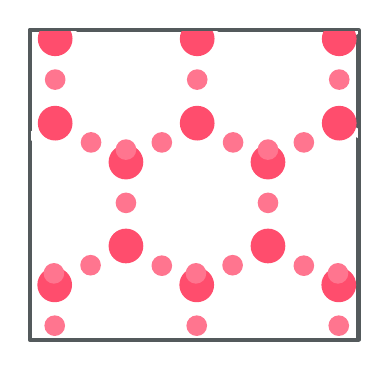
\begin{tikzpicture}[y=1cm, x=1cm, scale=0.75, inner sep=0pt, outer sep=0pt]
		\begin{scope}[shift={(-1.3062, 10.8309)}]

			\path[draw=pag!80,line join=round,line width=0.0521cm,miter limit=4.0] (1.3172, -5.572) rectangle (6.8838, -10.8199);

			\begin{scope}

				\clip (1.3172, -5.572) rectangle (6.8838, -10.8199);

				% 

				\path[draw=white,line cap=butt,line join=miter,line width=0.1058cm,miter limit=4.0,shift={(-1.8191, -7.0453)}] (7.1436, -2.1806) -- (6.5463, -2.5052);

				\path[draw=white,line cap=butt,line join=miter,line width=0.1058cm,miter limit=4.0,shift={(-1.8191, -7.0453)}] (7.754, -2.5182) -- (7.1566, -2.1806);

				\path[draw=white,line cap=butt,line join=miter,line width=0.1058cm,miter limit=4.0,shift={(-1.8191, -7.0453)}] (4.7518, -2.1806) -- (4.1545, -2.5052);

				\path[draw=white,line cap=butt,line join=miter,line width=0.1058cm,miter limit=4.0,shift={(-1.8191, -7.0453)}] (5.3621, -2.5182) -- (4.7648, -2.1806);

				\path[draw=white,line cap=butt,line join=miter,line width=0.1058cm,miter limit=4.0,shift={(-1.8191, -7.0453)}] (8.3648, -2.8614) -- (8.3753, -3.5611);

				\path[draw=white,line cap=butt,line join=miter,line width=0.1058cm,miter limit=4.0,shift={(-1.8191, -7.0453)}] (5.9518, -2.8614) -- (5.9623, -3.5611);

				\path[draw=white,line cap=butt,line join=miter,line width=0.1058cm,miter limit=4.0,shift={(-1.8191, -7.0453)}] (3.56, -2.8614) -- (3.5704, -3.5611);

				\path[draw=white,line cap=butt,line join=miter,line width=0.1058cm,miter limit=4.0,shift={(-1.8191, -7.0453)}] (7.1583, -0.787) -- (7.1688, -1.4868);

				\path[draw=white,line cap=butt,line join=miter,line width=0.1058cm,miter limit=4.0,shift={(-1.8191, -7.0453)}] (4.7453, -0.787) -- (4.7558, -1.4868);

				\path[draw=white,line cap=butt,line join=miter,line width=0.1058cm,miter limit=4.0,shift={(-1.8191, -7.0453)}] (8.3713, -0.1063) -- (7.774, -0.4309);

				\path[draw=white,line cap=butt,line join=miter,line width=0.1058cm,miter limit=4.0,shift={(-1.8191, -7.0453)}] (8.9816, -0.4439) -- (8.3843, -0.1063);

				\path[draw=white,line cap=butt,line join=miter,line width=0.127cm,miter limit=4.0,shift={(-1.8191, -7.0453)}] (8.3753, 1.3088) -- (8.9601, 1.6639);

				\path[draw=white,line cap=butt,line join=miter,line width=0.1058cm,miter limit=4.0,shift={(-1.8191, -7.0453)}] (8.3648, 1.3296) -- (8.3753, 0.6299);

				\path[draw=white,line cap=butt,line join=miter,line width=0.1058cm,miter limit=4.0,shift={(-1.8191, -7.0453)}] (5.9583, -0.1063) -- (5.361, -0.4309);

				\path[draw=white,line cap=butt,line join=miter,line width=0.1058cm,miter limit=4.0,shift={(-1.8191, -7.0453)}] (6.5686, -0.4439) -- (5.9713, -0.1063);

				\path[draw=white,line cap=butt,line join=miter,line width=0.1058cm,miter limit=4.0,shift={(-1.8191, -7.0453)}] (5.9623, 1.3088) -- (6.5471, 1.6639);

				\path[draw=white,line cap=butt,line join=miter,line width=0.1058cm,miter limit=4.0,shift={(-1.8191, -7.0453)}] (5.9518, 1.3296) -- (5.9623, 0.6299);

				\path[draw=white,line cap=butt,line join=miter,line width=0.1058cm,miter limit=4.0,shift={(-1.8191, -7.0453)}] (3.5665, -0.1063) -- (2.9691, -0.4309);

				\path[draw=white,line cap=butt,line join=miter,line width=0.1058cm,miter limit=4.0,shift={(-1.8191, -7.0453)}] (4.1768, -0.4439) -- (3.5794, -0.1063);

				\path[draw=white,line cap=butt,line join=miter,line width=0.1058cm,miter limit=4.0,shift={(-1.8191, -7.0453)}] (3.5704, 1.3088) -- (4.1553, 1.6639);

				\path[draw=white,line cap=butt,line join=miter,line width=0.1058cm,miter limit=4.0,shift={(-1.8191, -7.0453)}] (3.56, 1.3296) -- (3.5704, 0.6299);

				% 

				% 

				\path[fill=cff4d6d,cm={ 0.3,-0.0,-0.0,0.3,(0.2796, -6.3682)}] (5.8738, -2.6207).. controls (5.8738, -3.1614) and (5.4355, -3.5997) .. (4.8948, -3.5997).. controls (4.3541, -3.5997) and (3.9158, -3.1614) .. (3.9158, -2.6207).. controls (3.9158, -2.0801) and (4.3541, -1.6418) .. (4.8948, -1.6418).. controls (5.4355, -1.6418) and (5.8738, -2.0801) .. (5.8738, -2.6207) -- cycle;

				\path[fill=cff758f,cm={ 0.1784,-0.0,-0.0,0.1784,(2.6807, -7.0125)}] (5.8738, -2.6207).. controls (5.8738, -3.1614) and (5.4355, -3.5997) .. (4.8948, -3.5997).. controls (4.3541, -3.5997) and (3.9158, -3.1614) .. (3.9158, -2.6207).. controls (3.9158, -2.0801) and (4.3541, -1.6418) .. (4.8948, -1.6418).. controls (5.4355, -1.6418) and (5.8738, -2.0801) .. (5.8738, -2.6207) -- cycle;

				\path[fill=cff4d6d,cm={ 0.3,-0.0,-0.0,0.3,(2.6846, -6.3682)}] (5.8738, -2.6207).. controls (5.8738, -3.1614) and (5.4355, -3.5997) .. (4.8948, -3.5997).. controls (4.3541, -3.5997) and (3.9158, -3.1614) .. (3.9158, -2.6207).. controls (3.9158, -2.0801) and (4.3541, -1.6418) .. (4.8948, -1.6418).. controls (5.4355, -1.6418) and (5.8738, -2.0801) .. (5.8738, -2.6207) -- cycle;

				\path[fill=cff4d6d,cm={ 0.3,-0.0,-0.0,0.3,(1.4781, -7.027)}] (5.8738, -2.6207).. controls (5.8738, -3.1614) and (5.4355, -3.5997) .. (4.8948, -3.5997).. controls (4.3541, -3.5997) and (3.9158, -3.1614) .. (3.9158, -2.6207).. controls (3.9158, -2.0801) and (4.3541, -1.6418) .. (4.8948, -1.6418).. controls (5.4355, -1.6418) and (5.8738, -2.0801) .. (5.8738, -2.6207) -- cycle;

				\path[fill=cff758f,cm={ 0.1784,-0.0,-0.0,0.1784,(2.0735, -8.0364)}] (5.8738, -2.6207).. controls (5.8738, -3.1614) and (5.4355, -3.5997) .. (4.8948, -3.5997).. controls (4.3541, -3.5997) and (3.9158, -3.1614) .. (3.9158, -2.6207).. controls (3.9158, -2.0801) and (4.3541, -1.6418) .. (4.8948, -1.6418).. controls (5.4355, -1.6418) and (5.8738, -2.0801) .. (5.8738, -2.6207) -- cycle;

				\path[fill=cff758f,cm={ 0.1784,-0.0,-0.0,0.1784,(2.6807, -9.1)}] (5.8738, -2.6207).. controls (5.8738, -3.1614) and (5.4355, -3.5997) .. (4.8948, -3.5997).. controls (4.3541, -3.5997) and (3.9158, -3.1614) .. (3.9158, -2.6207).. controls (3.9158, -2.0801) and (4.3541, -1.6418) .. (4.8948, -1.6418).. controls (5.4355, -1.6418) and (5.8738, -2.0801) .. (5.8738, -2.6207) -- cycle;

				\path[fill=cff758f,cm={ 0.1784,-0.0,-0.0,0.1784,(5.0857, -7.0125)}] (5.8738, -2.6207).. controls (5.8738, -3.1614) and (5.4355, -3.5997) .. (4.8948, -3.5997).. controls (4.3541, -3.5997) and (3.9158, -3.1614) .. (3.9158, -2.6207).. controls (3.9158, -2.0801) and (4.3541, -1.6418) .. (4.8948, -1.6418).. controls (5.4355, -1.6418) and (5.8738, -2.0801) .. (5.8738, -2.6207) -- cycle;

				\path[fill=cff4d6d,cm={ 0.3,-0.0,-0.0,0.3,(5.0897, -6.3682)}] (5.8738, -2.6207).. controls (5.8738, -3.1614) and (5.4355, -3.5997) .. (4.8948, -3.5997).. controls (4.3541, -3.5997) and (3.9158, -3.1614) .. (3.9158, -2.6207).. controls (3.9158, -2.0801) and (4.3541, -1.6418) .. (4.8948, -1.6418).. controls (5.4355, -1.6418) and (5.8738, -2.0801) .. (5.8738, -2.6207) -- cycle;

				\path[fill=cff4d6d,cm={ 0.3,-0.0,-0.0,0.3,(3.8832, -7.027)}] (5.8738, -2.6207).. controls (5.8738, -3.1614) and (5.4355, -3.5997) .. (4.8948, -3.5997).. controls (4.3541, -3.5997) and (3.9158, -3.1614) .. (3.9158, -2.6207).. controls (3.9158, -2.0801) and (4.3541, -1.6418) .. (4.8948, -1.6418).. controls (5.4355, -1.6418) and (5.8738, -2.0801) .. (5.8738, -2.6207) -- cycle;

				\path[fill=cff758f,cm={ 0.1784,-0.0,-0.0,0.1784,(4.4785, -8.0364)}] (5.8738, -2.6207).. controls (5.8738, -3.1614) and (5.4355, -3.5997) .. (4.8948, -3.5997).. controls (4.3541, -3.5997) and (3.9158, -3.1614) .. (3.9158, -2.6207).. controls (3.9158, -2.0801) and (4.3541, -1.6418) .. (4.8948, -1.6418).. controls (5.4355, -1.6418) and (5.8738, -2.0801) .. (5.8738, -2.6207) -- cycle;

				\path[fill=cff758f,cm={ 0.1784,-0.0,-0.0,0.1784,(5.0857, -9.1)}] (5.8738, -2.6207).. controls (5.8738, -3.1614) and (5.4355, -3.5997) .. (4.8948, -3.5997).. controls (4.3541, -3.5997) and (3.9158, -3.1614) .. (3.9158, -2.6207).. controls (3.9158, -2.0801) and (4.3541, -1.6418) .. (4.8948, -1.6418).. controls (5.4355, -1.6418) and (5.8738, -2.0801) .. (5.8738, -2.6207) -- cycle;

				\path[fill=cff4d6d,cm={ 0.3,-0.0,-0.0,0.3,(0.2796, -4.9394)}] (5.8738, -2.6207).. controls (5.8738, -3.1614) and (5.4355, -3.5997) .. (4.8948, -3.5997).. controls (4.3541, -3.5997) and (3.9158, -3.1614) .. (3.9158, -2.6207).. controls (3.9158, -2.0801) and (4.3541, -1.6418) .. (4.8948, -1.6418).. controls (5.4355, -1.6418) and (5.8738, -2.0801) .. (5.8738, -2.6207) -- cycle;

				\path[fill=cff758f,cm={ 0.1784,-0.0,-0.0,0.1784,(0.8749, -5.9488)}] (5.8738, -2.6207).. controls (5.8738, -3.1614) and (5.4355, -3.5997) .. (4.8948, -3.5997).. controls (4.3541, -3.5997) and (3.9158, -3.1614) .. (3.9158, -2.6207).. controls (3.9158, -2.0801) and (4.3541, -1.6418) .. (4.8948, -1.6418).. controls (5.4355, -1.6418) and (5.8738, -2.0801) .. (5.8738, -2.6207) -- cycle;

				\path[fill=cff758f,cm={ 0.1784,-0.0,-0.0,0.1784,(1.4821, -7.0125)}] (5.8738, -2.6207).. controls (5.8738, -3.1614) and (5.4355, -3.5997) .. (4.8948, -3.5997).. controls (4.3541, -3.5997) and (3.9158, -3.1614) .. (3.9158, -2.6207).. controls (3.9158, -2.0801) and (4.3541, -1.6418) .. (4.8948, -1.6418).. controls (5.4355, -1.6418) and (5.8738, -2.0801) .. (5.8738, -2.6207) -- cycle;

				\path[fill=cff4d6d,cm={ 0.3,-0.0,-0.0,0.3,(2.6846, -4.9394)}] (5.8738, -2.6207).. controls (5.8738, -3.1614) and (5.4355, -3.5997) .. (4.8948, -3.5997).. controls (4.3541, -3.5997) and (3.9158, -3.1614) .. (3.9158, -2.6207).. controls (3.9158, -2.0801) and (4.3541, -1.6418) .. (4.8948, -1.6418).. controls (5.4355, -1.6418) and (5.8738, -2.0801) .. (5.8738, -2.6207) -- cycle;

				\path[fill=cff758f,cm={ 0.1784,-0.0,-0.0,0.1784,(3.28, -5.9488)}] (5.8738, -2.6207).. controls (5.8738, -3.1614) and (5.4355, -3.5997) .. (4.8948, -3.5997).. controls (4.3541, -3.5997) and (3.9158, -3.1614) .. (3.9158, -2.6207).. controls (3.9158, -2.0801) and (4.3541, -1.6418) .. (4.8948, -1.6418).. controls (5.4355, -1.6418) and (5.8738, -2.0801) .. (5.8738, -2.6207) -- cycle;

				\path[fill=cff758f,cm={ 0.1784,-0.0,-0.0,0.1784,(3.8872, -7.0125)}] (5.8738, -2.6207).. controls (5.8738, -3.1614) and (5.4355, -3.5997) .. (4.8948, -3.5997).. controls (4.3541, -3.5997) and (3.9158, -3.1614) .. (3.9158, -2.6207).. controls (3.9158, -2.0801) and (4.3541, -1.6418) .. (4.8948, -1.6418).. controls (5.4355, -1.6418) and (5.8738, -2.0801) .. (5.8738, -2.6207) -- cycle;

				\path[fill=cff4d6d,cm={ 0.3,-0.0,-0.0,0.3,(5.0897, -4.9394)}] (5.8738, -2.6207).. controls (5.8738, -3.1614) and (5.4355, -3.5997) .. (4.8948, -3.5997).. controls (4.3541, -3.5997) and (3.9158, -3.1614) .. (3.9158, -2.6207).. controls (3.9158, -2.0801) and (4.3541, -1.6418) .. (4.8948, -1.6418).. controls (5.4355, -1.6418) and (5.8738, -2.0801) .. (5.8738, -2.6207) -- cycle;

				\path[fill=cff758f,cm={ 0.1784,-0.0,-0.0,0.1784,(5.685, -5.9488)}] (5.8738, -2.6207).. controls (5.8738, -3.1614) and (5.4355, -3.5997) .. (4.8948, -3.5997).. controls (4.3541, -3.5997) and (3.9158, -3.1614) .. (3.9158, -2.6207).. controls (3.9158, -2.0801) and (4.3541, -1.6418) .. (4.8948, -1.6418).. controls (5.4355, -1.6418) and (5.8738, -2.0801) .. (5.8738, -2.6207) -- cycle;

				\path[fill=cff758f,cm={ 0.1784,-0.0,-0.0,0.1784,(1.4742, -9.0921)}] (5.8738, -2.6207).. controls (5.8738, -3.1614) and (5.4355, -3.5997) .. (4.8948, -3.5997).. controls (4.3541, -3.5997) and (3.9158, -3.1614) .. (3.9158, -2.6207).. controls (3.9158, -2.0801) and (4.3541, -1.6418) .. (4.8948, -1.6418).. controls (5.4355, -1.6418) and (5.8738, -2.0801) .. (5.8738, -2.6207) -- cycle;

				\path[fill=cff4d6d,cm={ 0.3,-0.0,-0.0,0.3,(1.4781, -8.4478)}] (5.8738, -2.6207).. controls (5.8738, -3.1614) and (5.4355, -3.5997) .. (4.8948, -3.5997).. controls (4.3541, -3.5997) and (3.9158, -3.1614) .. (3.9158, -2.6207).. controls (3.9158, -2.0801) and (4.3541, -1.6418) .. (4.8948, -1.6418).. controls (5.4355, -1.6418) and (5.8738, -2.0801) .. (5.8738, -2.6207) -- cycle;

				\path[fill=cff4d6d,cm={ 0.3,-0.0,-0.0,0.3,(0.2716, -9.1066)}] (5.8738, -2.6207).. controls (5.8738, -3.1614) and (5.4355, -3.5997) .. (4.8948, -3.5997).. controls (4.3541, -3.5997) and (3.9158, -3.1614) .. (3.9158, -2.6207).. controls (3.9158, -2.0801) and (4.3541, -1.6418) .. (4.8948, -1.6418).. controls (5.4355, -1.6418) and (5.8738, -2.0801) .. (5.8738, -2.6207) -- cycle;

				\path[fill=cff758f,cm={ 0.1784,-0.0,-0.0,0.1784,(0.867, -10.116)}] (5.8738, -2.6207).. controls (5.8738, -3.1614) and (5.4355, -3.5997) .. (4.8948, -3.5997).. controls (4.3541, -3.5997) and (3.9158, -3.1614) .. (3.9158, -2.6207).. controls (3.9158, -2.0801) and (4.3541, -1.6418) .. (4.8948, -1.6418).. controls (5.4355, -1.6418) and (5.8738, -2.0801) .. (5.8738, -2.6207) -- cycle;

				\path[fill=cff758f,cm={ 0.1784,-0.0,-0.0,0.1784,(3.8792, -9.0921)}] (5.8738, -2.6207).. controls (5.8738, -3.1614) and (5.4355, -3.5997) .. (4.8948, -3.5997).. controls (4.3541, -3.5997) and (3.9158, -3.1614) .. (3.9158, -2.6207).. controls (3.9158, -2.0801) and (4.3541, -1.6418) .. (4.8948, -1.6418).. controls (5.4355, -1.6418) and (5.8738, -2.0801) .. (5.8738, -2.6207) -- cycle;

				\path[fill=cff4d6d,cm={ 0.3,-0.0,-0.0,0.3,(3.8832, -8.4478)}] (5.8738, -2.6207).. controls (5.8738, -3.1614) and (5.4355, -3.5997) .. (4.8948, -3.5997).. controls (4.3541, -3.5997) and (3.9158, -3.1614) .. (3.9158, -2.6207).. controls (3.9158, -2.0801) and (4.3541, -1.6418) .. (4.8948, -1.6418).. controls (5.4355, -1.6418) and (5.8738, -2.0801) .. (5.8738, -2.6207) -- cycle;

				\path[fill=cff4d6d,cm={ 0.3,-0.0,-0.0,0.3,(2.6767, -9.1066)}] (5.8738, -2.6207).. controls (5.8738, -3.1614) and (5.4355, -3.5997) .. (4.8948, -3.5997).. controls (4.3541, -3.5997) and (3.9158, -3.1614) .. (3.9158, -2.6207).. controls (3.9158, -2.0801) and (4.3541, -1.6418) .. (4.8948, -1.6418).. controls (5.4355, -1.6418) and (5.8738, -2.0801) .. (5.8738, -2.6207) -- cycle;

				\path[fill=cff758f,cm={ 0.1784,-0.0,-0.0,0.1784,(3.272, -10.116)}] (5.8738, -2.6207).. controls (5.8738, -3.1614) and (5.4355, -3.5997) .. (4.8948, -3.5997).. controls (4.3541, -3.5997) and (3.9158, -3.1614) .. (3.9158, -2.6207).. controls (3.9158, -2.0801) and (4.3541, -1.6418) .. (4.8948, -1.6418).. controls (5.4355, -1.6418) and (5.8738, -2.0801) .. (5.8738, -2.6207) -- cycle;

				\path[fill=cff4d6d,cm={ 0.3,-0.0,-0.0,0.3,(5.0818, -9.1066)}] (5.8738, -2.6207).. controls (5.8738, -3.1614) and (5.4355, -3.5997) .. (4.8948, -3.5997).. controls (4.3541, -3.5997) and (3.9158, -3.1614) .. (3.9158, -2.6207).. controls (3.9158, -2.0801) and (4.3541, -1.6418) .. (4.8948, -1.6418).. controls (5.4355, -1.6418) and (5.8738, -2.0801) .. (5.8738, -2.6207) -- cycle;

				\path[fill=cff758f,cm={ 0.1784,-0.0,-0.0,0.1784,(5.6771, -10.116)}] (5.8738, -2.6207).. controls (5.8738, -3.1614) and (5.4355, -3.5997) .. (4.8948, -3.5997).. controls (4.3541, -3.5997) and (3.9158, -3.1614) .. (3.9158, -2.6207).. controls (3.9158, -2.0801) and (4.3541, -1.6418) .. (4.8948, -1.6418).. controls (5.4355, -1.6418) and (5.8738, -2.0801) .. (5.8738, -2.6207) -- cycle;

				\path[fill=cff758f,cm={ 0.1784,-0.0,-0.0,0.1784,(2.0735, -7.1342)}] (5.8738, -2.6207).. controls (5.8738, -3.1614) and (5.4355, -3.5997) .. (4.8948, -3.5997).. controls (4.3541, -3.5997) and (3.9158, -3.1614) .. (3.9158, -2.6207).. controls (3.9158, -2.0801) and (4.3541, -1.6418) .. (4.8948, -1.6418).. controls (5.4355, -1.6418) and (5.8738, -2.0801) .. (5.8738, -2.6207) -- cycle;

				\path[fill=cff758f,cm={ 0.1784,-0.0,-0.0,0.1784,(4.4785, -7.1342)}] (5.8738, -2.6207).. controls (5.8738, -3.1614) and (5.4355, -3.5997) .. (4.8948, -3.5997).. controls (4.3541, -3.5997) and (3.9158, -3.1614) .. (3.9158, -2.6207).. controls (3.9158, -2.0801) and (4.3541, -1.6418) .. (4.8948, -1.6418).. controls (5.4355, -1.6418) and (5.8738, -2.0801) .. (5.8738, -2.6207) -- cycle;

				\path[fill=cff758f,cm={ 0.1784,-0.0,-0.0,0.1784,(0.8537, -9.2297)}] (5.8738, -2.6207).. controls (5.8738, -3.1614) and (5.4355, -3.5997) .. (4.8948, -3.5997).. controls (4.3541, -3.5997) and (3.9158, -3.1614) .. (3.9158, -2.6207).. controls (3.9158, -2.0801) and (4.3541, -1.6418) .. (4.8948, -1.6418).. controls (5.4355, -1.6418) and (5.8738, -2.0801) .. (5.8738, -2.6207) -- cycle;

				\path[fill=cff758f,cm={ 0.1784,-0.0,-0.0,0.1784,(3.2588, -9.2297)}] (5.8738, -2.6207).. controls (5.8738, -3.1614) and (5.4355, -3.5997) .. (4.8948, -3.5997).. controls (4.3541, -3.5997) and (3.9158, -3.1614) .. (3.9158, -2.6207).. controls (3.9158, -2.0801) and (4.3541, -1.6418) .. (4.8948, -1.6418).. controls (5.4355, -1.6418) and (5.8738, -2.0801) .. (5.8738, -2.6207) -- cycle;

				\path[fill=cff758f,cm={ 0.1784,-0.0,-0.0,0.1784,(5.6638, -9.2297)}] (5.8738, -2.6207).. controls (5.8738, -3.1614) and (5.4355, -3.5997) .. (4.8948, -3.5997).. controls (4.3541, -3.5997) and (3.9158, -3.1614) .. (3.9158, -2.6207).. controls (3.9158, -2.0801) and (4.3541, -1.6418) .. (4.8948, -1.6418).. controls (5.4355, -1.6418) and (5.8738, -2.0801) .. (5.8738, -2.6207) -- cycle;
			\end{scope}
			% 

			\path[draw=pag!80,line join=round,line width=0.0221cm,miter limit=4.0] (1.3172, -5.572) rectangle (6.8838, -10.8199);

		\end{scope}

	\end{tikzpicture}
\end{minipage}
\pagebreak

\noindent\textbf{Energy Changes} - Different state changes have different names. When the system gains energy, the phase is increased as greater kinetic energy is enables the system to overcome intermolecular forces. The opposite occurs when the phase is lowered.  Some examples of this can be seen below\\

\hspace{-30pt}\begin{minipage}{0.435\textwidth}

	\begin{itemize}
		\item \textbf{Sweat} - Sweat leaving our body turns to gas. The phase change absorbs energy from our tissues, resultant in cooling of the body.
		\item \textbf{Vapor Burn} - Burning your hand with steam is the change of water from a gas to a liquid. The energy emitted in the change of phases would injure your hand.
	\end{itemize}

\end{minipage}
\hspace{5pt}\begin{minipage}{0.7\textwidth}

	\renewcommand{\Tstrut}{\rule{0pt}{3ex}}         % Top strut
	\renewcommand{\Bstrut}{\rule[1ex]{0pt}{0pt}}   % Bottom strut
	\renewcommand{\TBstrut}{\Tstrut\Bstrut}
	\newcommand{\TTstrut}{\rule{0pt}{1ex}}         % Top strut
	\newcommand{\BBstrut}{\rule[1ex]{0pt}{0pt}}   % Bottom strut
	\newcommand{\TTBBstrut}{\Tstrut\Bstrut}
	\begin{tabular}{l@{\qquad\quad}l@{\qquad\quad}l}
		\hline
		\textbf{Process} & \textbf{State Change}                                                            & \textbf{Reaction type}                    \\
		\hline
		Melting          & \textcolor{red1!80!pag}{Solid} $\longrightarrow$ \textcolor{red3!80!pag}{Liquid} & \textcolor{pag!50}{Endothermic}\TBstrut   \\
		Freezing         & \textcolor{red3!80!pag}{Liquid} $\longrightarrow$ \textcolor{red1!80!pag}{Solid} & \textcolor{pag!50}{Exothermic} \TTBBstrut \\
		Vaporization     & \textcolor{red3!80!pag}{Liquid} $\longrightarrow$ \textcolor{red5!80!pag}{Gas}   & \textcolor{pag!50}{Endothermic}\TTBBstrut \\
		Condensation     & \textcolor{red5!80!pag}{Gas} $\longrightarrow$ \textcolor{red3!80!pag}{Liquid}   & \textcolor{pag!50}{Exothermic}\TTBBstrut  \\
		Sublimation      & \textcolor{red1!80!pag}{Solid} $\longrightarrow$ \textcolor{red5!80!pag}{Gas}    & \textcolor{pag!50}{Endothermic}\TTBBstrut \\
		Deposition       & \textcolor{red5!80!pag}{Gas} $\longrightarrow$ \textcolor{red1!80!pag}{Solid}    & \textcolor{pag!50}{Exothermic}\TTBBstrut  \\
		\hline
	\end{tabular}

\end{minipage}

\vspace{15pt}
\noindent\textbf{Magnitude of Enthalpy Change} - The change in enthalpy between two phases will be different for different substances. This difference represents the interparticle forces and there strengths. The enthalpy change in fusion, or going from a solid to a liquid, is denoted as $\Delta H^{\circ}_{fus}$, while the enthalpy change in vaporization is denoted as $\Delta H^{\circ}_{vap}$. These are both measured in $\frac{\text{kJ}}{\text{mol}}$. For the solid-gas phase changes, we can calculate change in enthalpy by simply summing the vaporization and fusion enthalpies. Chemicals that have hydrogen tend to remain a liquid because of the strong hydrogen intermolecular forces.\\
\\
In general, the energy required for vaporization is much higher then the energy required for fusion. One good analogy is a bucket of metal ball bearings. If you started stirring it with your hand, it would require a moderate amount of energy. This would be the liquid phase. To get to the gas phase however, it would be the equivalent of throwing the bucket into the air such that each ball bearing is randomly dispersed. Obviously, the second change would require more energy. \\
\\
\textbf{Phase Change Equilibrium} - In an open system, phase change is not reversible, as energy lost is permanently lost. However, with an closed system, the energy is conserved. While phase change continues to occur, it is not limited to one direction. Instead, we get an equilibrium, where the particles switch between phases until a balance is met. In the example below, an open system containing liquid is put under a vacuum, converting it to a closed system. Given enough time, gas begins to form.
\vspace{15pt}

\begin{minipage}{25cm}
	\begin{center}
		\tdplotsetmaincoords{70}{165}
		\newcommand{\randomnessfactor}{0.05}
		\hspace{-9.2cm}	\begin{tikzpicture}
			[tdplot_main_coords,
				grid/.style={very thin,gray},
				axis/.style={->,blue,thick},
				cube/.style={opacity=.5,very thick,},scale=2]
			% draw a grid in the x-y plane
			\foreach \x in {1,1.5,...,3.5}
			\foreach \y in {1,1.5,...,3.5}
				{
					\draw[grid] (\x,1) -- (\x,3.5);
					\draw[grid] (1,\y) -- (3.5,\y);
				}
			% draw the bottom of the cube
			\draw[cube,thin] (1.5,1.5,0) -- (1.5,3,0) -- (3,3,0) -- (3,1.5,0) -- cycle;

			% draw the back-right of the cube
			\draw[cube,thin] (1.5,1.5,0) -- (1.5,3,0) -- (1.5,3,2) -- (1.5,1.5,2) -- cycle;

			% draw the back-left of the cube
			\draw[cube,thin] (1.5,1.5,0) -- (3,1.5,0) -- (3,1.5,2) -- (1.5,1.5,2) -- cycle;

			\foreach \z in {0,0.1,...,0.45}
			\foreach \x in {1.6,1.65,...,2.9}
			\foreach \y in {1.6,1.65,...,2.9}{\pgfmathsetmacro{\myangle}{360*rnd}
					\pic at ({\x+(\randomnessfactor*rand)},{\y+(\randomnessfactor*rand)},{0.05+\z+(0.05*rand/2)}) {threedballsthree}; }

			\foreach \z in {0,0.025,...,0.5}
			\foreach \x in {1.6,1.65,...,2.9}
			\foreach \y in {2.9}{\pgfmathsetmacro{\myangle}{360*rnd}
					\pic at ({\x+(\randomnessfactor*rand)},{\y},{0.05+\z+(0.05*rand)}) {threedballsthree}; }
			% draw the axes
			\foreach \z in {0,0.025,...,0.45}
			\foreach \x in {2.9}
			\foreach \y in {1.6,1.7,...,2.9}{\pgfmathsetmacro{\myangle}{360*rnd}
					\pic at ({\x},{\y+(\randomnessfactor*rand)},{0.05+\z+(0.05*rand)}) {threedballsthree}; }

			\foreach \z in {0.5}
			\foreach \x in {1.6,1.65,...,2.9}
			\foreach \y in {1.6,1.65,...,2.9}{\pgfmathsetmacro{\myangle}{360*rnd}
					\pic at ({\x+(\randomnessfactor*rand)},{\y+(\randomnessfactor*rand)},{\z}) {threedballsthree}; }

			% draw the front-right of the cube
			% draw the front-right of the cube
			\draw[cube,thin] (3,1.5,0) -- (3,3,0) -- (3,3,2) -- (3,1.5,2) -- cycle;

			% draw the front-left of the cube
			\draw[cube,thin] (1.5,3,0) -- (3,3,0) -- (3,3,2) -- (1.5,3,2) -- cycle;

			% draw the top of the cube
			\draw[cube,thin] (1.5,1.5,2) -- (1.5,3,2) -- (3,3,2) -- (3,1.5,2) -- cycle;

		\end{tikzpicture}
		\hspace{5pt}\begin{tikzpicture}
			[tdplot_main_coords,
				grid/.style={very thin,gray},
				axis/.style={->,blue,thick},
				cube/.style={opacity=.5,very thick,},scale=2]
			% draw a grid in the x-y plane
			\foreach \x in {1,1.5,...,3.5}
			\foreach \y in {1,1.5,...,3.5}
				{
					\draw[grid] (\x,1) -- (\x,3.5);
					\draw[grid] (1,\y) -- (3.5,\y);
				}
			% draw the bottom of the cube
			\draw[cube,fill=pag!80,thin] (1.5,1.5,0) -- (1.5,3,0) -- (3,3,0) -- (3,1.5,0) -- cycle;

			% draw the back-right of the cube
			\draw[cube,fill=pag!80,thin] (1.5,1.5,0) -- (1.5,3,0) -- (1.5,3,2) -- (1.5,1.5,2) -- cycle;

			% draw the back-left of the cube
			\draw[cube,fill=pag!80,thin] (1.5,1.5,0) -- (3,1.5,0) -- (3,1.5,2) -- (1.5,1.5,2) -- cycle;

			\foreach \z in {0,0.1,...,0.45}
			\foreach \x in {1.6,1.65,...,2.9}
			\foreach \y in {1.6,1.65,...,2.9}{\pgfmathsetmacro{\myangle}{360*rnd}
					\pic at ({\x+(\randomnessfactor*rand)},{\y+(\randomnessfactor*rand)},{0.05+\z+(0.05*rand/2)}) {threedballsthree}; }

			\foreach \z in {0,0.025,...,0.5}
			\foreach \x in {1.6,1.65,...,2.9}
			\foreach \y in {2.9}{\pgfmathsetmacro{\myangle}{360*rnd}
					\pic at ({\x+(\randomnessfactor*rand)},{\y},{0.05+\z+(0.05*rand)}) {threedballsthree}; }
			% draw the axes
			\foreach \z in {0,0.025,...,0.45}
			\foreach \x in {2.9}
			\foreach \y in {1.6,1.7,...,2.9}{\pgfmathsetmacro{\myangle}{360*rnd}
					\pic at ({\x},{\y+(\randomnessfactor*rand)},{0.05+\z+(0.05*rand)}) {threedballsthree}; }

			\foreach \z in {0.5}
			\foreach \x in {1.6,1.65,...,2.9}
			\foreach \y in {1.6,1.65,...,2.9}{\pgfmathsetmacro{\myangle}{360*rnd}
					\pic at ({\x+(\randomnessfactor*rand)},{\y+(\randomnessfactor*rand)},{\z}) {threedballsthree}; }

			% draw the front-right of the cube
			% draw the front-right of the cube
			\draw[cube,thin] (3,1.5,0) -- (3,3,0) -- (3,3,2) -- (3,1.5,2) -- cycle;

			% draw the front-left of the cube
			\draw[cube,thin] (1.5,3,0) -- (3,3,0) -- (3,3,2) -- (1.5,3,2) -- cycle;

			% draw the top of the cube
			\draw[cube,thin] (1.5,1.5,2) -- (1.5,3,2) -- (3,3,2) -- (3,1.5,2) -- cycle;

		\end{tikzpicture}
		\hspace{5pt}\begin{tikzpicture}
			[tdplot_main_coords,
				grid/.style={very thin,gray},
				axis/.style={->,blue,thick},
				cube/.style={opacity=.5,very thick,},scale=2]
			% draw a grid in the x-y plane
			\foreach \x in {1,1.5,...,3.5}
			\foreach \y in {1,1.5,...,3.5}
				{
					\draw[grid] (\x,1) -- (\x,3.5);
					\draw[grid] (1,\y) -- (3.5,\y);
				}
			% draw the bottom of the cube
			\draw[cube,fill=pag!80,thin] (1.5,1.5,0) -- (1.5,3,0) -- (3,3,0) -- (3,1.5,0) -- cycle;

			% draw the back-right of the cube
			\draw[cube,fill=pag!80,thin] (1.5,1.5,0) -- (1.5,3,0) -- (1.5,3,2) -- (1.5,1.5,2) -- cycle;

			% draw the back-left of the cube
			\draw[cube,fill=pag!80,thin] (1.5,1.5,0) -- (3,1.5,0) -- (3,1.5,2) -- (1.5,1.5,2) -- cycle;

			% draw the axes
			\foreach \z in {0.25,0.65,...,2}
			\foreach \x in {1.6,1.8,...,2.9}
			\foreach \y in {1.6,1.8,...,2.9}{\pgfmathsetmacro{\myangle}{360*rnd}
					\pic at ({\x+(0.1*rand)},{\y+(0.1*rand)},{0.05+\z+(0.05*rand/2)}) {threedballsthree}; }

			\foreach \z in {0,0.1,...,0.35}
			\foreach \x in {1.6,1.65,...,2.9}
			\foreach \y in {1.6,1.65,...,2.9}{\pgfmathsetmacro{\myangle}{360*rnd}
					\pic at ({\x+(\randomnessfactor*rand)},{\y+(\randomnessfactor*rand)},{0.05+\z+(0.05*rand/2)}) {threedballsthree}; }

			\foreach \z in {0,0.025,...,0.35}
			\foreach \x in {1.6,1.65,...,2.9}
			\foreach \y in {2.9}{\pgfmathsetmacro{\myangle}{360*rnd}
					\pic at ({\x+(\randomnessfactor*rand)},{\y},{0.05+\z+(0.05*rand)}) {threedballsthree}; }
			% draw the axes
			\foreach \z in {0,0.025,...,0.35}
			\foreach \x in {2.9}
			\foreach \y in {1.6,1.7,...,2.9}{\pgfmathsetmacro{\myangle}{360*rnd}
					\pic at ({\x},{\y+(\randomnessfactor*rand)},{0.05+\z+(0.05*rand)}) {threedballsthree}; }

			\foreach \z in {0.35}
			\foreach \x in {1.6,1.65,...,2.9}
			\foreach \y in {1.6,1.65,...,2.9}{\pgfmathsetmacro{\myangle}{360*rnd}
					\pic at ({\x+(\randomnessfactor*rand)},{\y+(\randomnessfactor*rand)},{\z}) {threedballsthree}; }

			% draw the front-right of the cube
			% draw the front-right of the cube
			\draw[cube,thin] (3,1.5,0) -- (3,3,0) -- (3,3,2) -- (3,1.5,2) -- cycle;

			% draw the front-left of the cube
			\draw[cube,thin] (1.5,3,0) -- (3,3,0) -- (3,3,2) -- (1.5,3,2) -- cycle;

			% draw the top of the cube
			\draw[cube,thin] (1.5,1.5,2) -- (1.5,3,2) -- (3,3,2) -- (3,1.5,2) -- cycle;

		\end{tikzpicture}
	\end{center}
\end{minipage}

\vspace{15pt}

\pagebreak

\noindent\textbf{Vapor Pressure} - When this equilibrium point is reached, the vapor will have some constant pressure. We call this the vapor pressure, and it is different for different liquids at \textbf{constant temperatures}. A higher temperature will increase the vapor pressure. Calling back to earlier, in the graph below, the speed of a particle is plotted against the probability of that speed for different temperatures. After a certain speed, the particle will enter the gas phase, represented by the shaded area. As displayed, the amount of gaseous particles increases as the temperature increases. A system that does not have a high enough temperature will not produce any gaseous particles, as seen by the 50 Kelvin plot below.

\vspace{10pt}
\begin{center}

	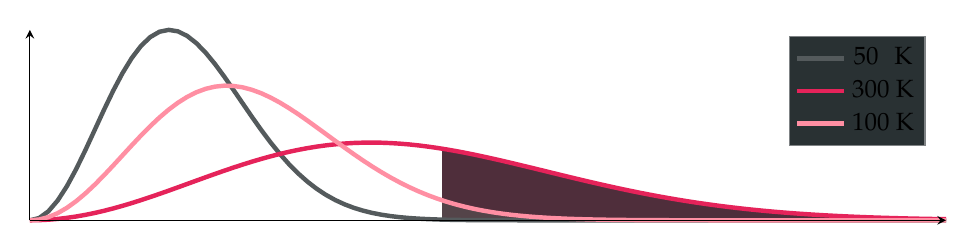
\begin{tikzpicture}[scale=1]
		\begin{axis}[
				axis lines=middle,
				xlabel=,
				ylabel={},
				legend style={
						fill=pag, draw=pag!60, % Red background with black border
						font=\small, % Smaller font size
						inner sep=2pt, % Inner spacing (padding around the text)
						outer sep=1pt  % Outer spacing (margin around the border)
					},
				domain=0:6000,
				xtick=\empty,
				ytick=\empty,
				grid=both,
				grid style={line width=.1pt, draw=gray!10},
				major grid style={line width=.2pt,draw=gray!50},
				minor tick num=5,
				width=1.09*\textwidth,
				height=4cm,
				clip=false,
				ticklabel style={font=\tiny,fill=white},
				xlabel style={at={(ticklabel* cs:1)},anchor=north west},
				ylabel style={at={(ticklabel* cs:1)},anchor=south west},
				axis on top,
			]
			% Function f(x) = 1/x

			% Main plot for legend - Plot 1

			% Main plot for legend - Plot 2
			\addplot [name path=ohwow, color=pag!80, ultra thick, samples=100] {\maxwellboltzmann{50}};
			\addlegendentry{50 $\:\:$K}

			\addplot [name path=wowow, color=red12, ultra thick, samples=100] {\maxwellboltzmann{300}};
			\addlegendentry{300 K}

			\addplot [name path=wow, color=red3, ultra thick, samples=100] {\maxwellboltzmann{100}};
			\addlegendentry{100 K}

			\addplot [name path=plot2, color=red12, ultra thick, samples=100, transparent] {\maxwellboltzmann{300}};

			\addplot [name path=plot1, color=red3, ultra thick, samples=100, transparent] {\maxwellboltzmann{100}};

			\path[name path=axis3] (axis cs:3000,0) -- (axis cs:6000,0);

			\path[name path=axis2] (axis cs:2700,0) -- (axis cs:6000,0);
			\addplot[red12!20!pag] fill between[of=plot2 and axis2, soft clip={domain=2700:6000}];

			\path[name path=axis1] (axis cs:2700,0) -- (axis cs:6000,0);
			\addplot[red3!20!pag] fill between[of=plot1 and axis1, soft clip={domain=2700:6000}];

		\end{axis}

	\end{tikzpicture}

\end{center}

\noindent\textbf{Open Systems} - Although phase	change is not reversible for open systems, there is still a threshold temperature at which boiling will occur. For an open system, the pressure has to overcome the vapor pressure for that liquid. In earths atmosphere, usually that pressure is 1 atm, but this can change depending on elevation. On Mount Everest for example, the boiling point of water is 69.94 $^{\circ} $C as there is less atmospheric pressure. Higher elevation means lower atmospheric pressure, which means a lower boiling point. Vapor pressure and boiling point are \textbf{inverse quantities}.\\
\\
Vapor pressure in an open system applies for all compounds. Something like Nitrogen has essentially no vapor pressure and boils at -196 $^{\circ}$C. Something like mercury has a very low vapor pressure, similar to water. This makes handling mercury so dangerous because it will evaporate and saturate the air in the same fashion that water would.

\vspace{10pt}
\renewcommand{\Tstrut}{\rule{0pt}{3.3ex}}         % Top strut
\renewcommand{\Bstrut}{\rule[-2ex]{0pt}{0pt}}   % Bottom strut
\renewcommand{\TBstrut}{\Tstrut\Bstrut}
\newcommand{\TTstrut}{\rule{0pt}{1ex}}         % Top strut
\newcommand{\BBstrut}{\rule[1ex]{0pt}{0pt}}   % Bottom strut
\newcommand{\TTBBstrut}{\Tstrut\Bstrut}
\hspace{-17pt}\begin{tabular}{|l|@{\qquad\quad}c@{\qquad\quad}c@{\qquad\quad}c@{\qquad\quad}c@{\qquad\quad}c@{\qquad\quad}|}
	\hline
	\textbf{Substance}                      & N$_2$ & (C$_2$H$_5$)$_2$O & C$_2$H$_5$OH & H$_2$O & Hg \TBstrut   \\
	\hline
	Vapor Pressure at 22 $^{\circ}$C (torr) & (N/A) & 450               & 45           & 20     & 10 \TTBBstrut \\
	Boiling Point ($^{\circ}$C)             & -196  & 35                & 78           & 100    & 357\TTBBstrut \\

	\hline
\end{tabular}

\vspace{15	pt}
\noindent\textbf{Other Phase Equilibrium} - Transitions between all phases occur, and as such have different equilibrium points. For solids turning to liquids, because of there near incompressibility, there tends not to be an effect on the threshold temperature by the pressure of a system. If the particle forces between some substance are low enough, that substance will jump directly to a gas (think dry ice / solid CO$_2$ or Iodine). We can have solid-gas, liquid solid, etc, etc equilibrium points.

\section*{\LARGE\uline{Phase Diagrams}}

\hspace{-28pt}\begin{minipage}{0.38\textwidth}

	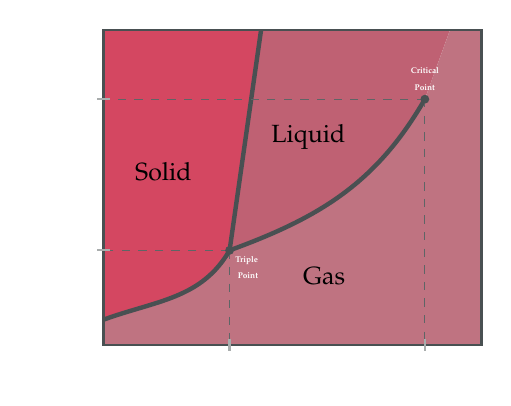
\begin{tikzpicture}[scale=0.4]
		\message{Phase diagrams^^J}

		\def\xtick#1#2{\draw[thick,pag!40] (#1)++(0,.2) --++ (0,-.4) node[below=-.5pt,scale=0.7, white] {#2};}
		\def\ytick#1#2{\draw[thick,pag!40] (#1)++(.2,0) --++ (-.4,0) node[white, left=-.5pt,scale=0.7] {#2};}

		% COORDINATES
		\coordinate (O) at (0,0);
		\coordinate (N1) at (5,10);
		\coordinate (N2) at (11,10);
		\coordinate (NE) at (12,10);
		\coordinate (NW) at (0,10);
		\coordinate (SE) at (12,0);
		\coordinate (W) at (0,5);
		\coordinate (S) at (6,0);
		\coordinate (C) at (10.2,7.8); % critical
		\coordinate (T) at (4,3); % triple
		\coordinate (C1) at (10.2,10);
		\coordinate (C1) at (12,7.8);
		\coordinate (R) at (0,0.8);
		% PATHS
		\def\SL{(T) -- (N1)}
		\def\SG{(R) to[out=20,in=-120] (T)}
		\def\LG{(T) to[out=20,in=-120] (C)}
		\def\atm{(0,5.5) -- (12,5.5)}
		\path[name path=SL] \SL;
		\path[name path=LG] \LG;
		\path[name path=atm] \atm;

		% REGIONS
		\fill[red5!80!pag] \SG -- (N1) -- (NW) -- cycle;
		\fill[red4!70!pag] \LG -- (N2) -- (N1) -- cycle;
		\fill[red3!70!pag] \LG -- (N2) -- (NE) -- (SE) -- (O) -- \SG --  cycle;
		\node at (1.9,5.5) {\small Solid};
		\node at (7,2.2) {\small Gas};
		\node at (6.5,6.6) {\small Liquid};

		% % MIXED
		% \shade[top color=mylightblue,bottom color=mylightred,shading angle=70]
		%  (10.4,7.7) -- (11.2,10) -- (10.8,10) -- (10.0,7.7) -- cycle;

		% POINTS

		% LINES
		\draw[ultra thick,pag!85] \SG;
		\draw[ultra thick,pag!85] \LG;
		\draw[ultra thick,pag!85] \SL;
		\draw[dashed,pag!75] (T) -- ($(T |- 0,0)$) coordinate (Tx);
		\draw[dashed,pag!75] (T) -- ($(T -| 0,0)$) coordinate (Ty);
		\draw[dashed,pag!75] (C) -- ($(C |- 0,0)$) coordinate (Cx);
		\draw[dashed,pag!75] (C) -- ($(C -| 0,0)$) coordinate (Cy);
		\fill[pag!85] (T) circle (4pt) node[below right,scale=0.6,align=right] {\tiny \textcolor{white}{\textbf{Triple}}\\[-2pt]\tiny\textcolor{white}{\textbf{Point}}};
		\fill[pag!85] (C) circle (4pt) node[above=1pt,scale=0.6,align=center] {\tiny\textcolor{white}{\textbf{Critical}}\\[-2pt]\tiny\textcolor{white}{\textbf{Point}}};

		% AXES
		\draw[thick,pag!85] (O) rectangle (NE);
		\xtick{Tx}{\hspace{9pt}-57$^{\circ}$C}
		\ytick{Ty}{5 atm}
		\xtick{Cx}{31 $^{\circ}$C}
		\ytick{Cy}{73 atm}

	\end{tikzpicture}
\end{minipage}
\begin{minipage}{0.67\textwidth}
	\textbf{Carbon Dioxide Phase Diagram} - To the left shows the phase diagram for carbon dioxide (CO$_2$). Phase diagrams allow us to visualize the relationship between the different states of matter, pressure and temperature. The lines represent areas of temperature and pressure where equilibrium will occur. When thinking about vapor pressure, when the gas is removed from a closed system, the pressure is very low. As such, gas begins to form. Eventually the pressure exerted by the gas will equalize itself at some point along the liquid-gas line in a phase diagram.  \\

\end{minipage}

\vspace{10pt}

\noindent\textbf{Lines} - The line between liquid and gases is called the vapor pressure line. Additionally, as described earlier, the pressure has very little effect on the melting point of a solid, which can be seen in phase diagrams. Liquids and solids are nearly incompressible, so any exponential curving of the line is nearly completely diminished giving us something linear. Finally, if the slope of this line is positive, it tells us that the substance in question has a higher density in its solid form then it does in its liquid form.\\
\\
\textbf{Critical Point} - The critical point is the point along the vapor pressure curve where the temperature and pressure for a substance in its liquid and gas forms are of equal density. Anything beyond these two parameters leads to a state of supercrticality. We call a substance in this state a \textbf{supercritical fluid}. It will exhibit both gas and liquid properties, and is effectively a combination of the two.\\
\\
\textbf{Triple Point} - The triple point is the point such that the balance between pressure and temperature results in a equilibrium between gas, liquid, and solid phases. A triple point above 1 atm means that the substance in question cannot exist  in the liquid liquid phase under standard atmospheric conditions, and sublimation will occur. \\
\\
\textbf{Decaffeinating Coffee Supercriticaly} - We can use supercritical CO2 to decaffeinate coffee. In its gas form, coffee has to much kinetic energy to have intermolecular reactions close enough to have any effect on the caffeine. In a liquid form, it cannot fully permeate the coffee beans the same way that a gas can. In its super critical state however, it has both strong enough inter molecular forces to draw out caffeine, and the ability to permeate the coffee beans completely, like a gas.

\vspace{20pt}
\hspace{-52pt}\begin{minipage}{0.47\textwidth}

	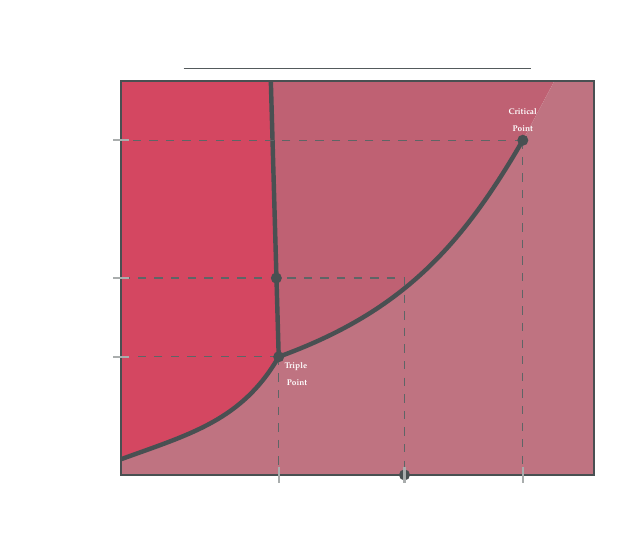
\begin{tikzpicture}[scale=0.5]
		\message{Phase diagrams^^J}

		\def\xtick#1#2{\draw[thick,pag!40] (#1)++(0,.2) --++ (0,-.4) node[below=-.5pt,scale=0.7, white] {#2};}
		\def\ytick#1#2{\draw[thick,pag!40] (#1)++(.2,0) --++ (-.4,0) node[white, left=-.5pt,scale=0.7] {#2};}

		% COORDINATES
		\coordinate (O) at (0,0);
		\coordinate (N1) at (3.8,10);
		\coordinate (N2) at (11,10);
		\coordinate (NE) at (12,10);
		\coordinate (NW) at (0,10);
		\coordinate (SE) at (12,0);
		\coordinate (W) at (0,5);
		\coordinate (S) at (6,0);
		\coordinate (C) at (10.2,8.5); % critical
		\coordinate (T) at (4,3); % triple
		\coordinate (C1) at (10.2,10);
		\coordinate (C1) at (12,7.8);
		\coordinate (M)  at (0,5);
		\coordinate (M1) at (3.94, 5);
		\coordinate (B) at (7.195, 5);
		\coordinate (B1) at (7.195, 0);
		\coordinate (R) at (0,0.4);
		% PATHS
		\def\SL{(T) -- (N1)}
		\def\SG{(R) to[out=20,in=-120] (T)}
		\def\LG{(T) to[out=20,in=-120] (C)}
		\def\atm{(0,5.5) -- (12,5.5)}
		\path[name path=SL] \SL;
		\path[name path=LG] \LG;
		\path[name path=atm] \atm;

		% REGIONS
		\fill[red5!80!pag] \SG -- (N1) -- (NW) -- cycle;
		\fill[red4!70!pag] \LG -- (N2) -- (N1) -- cycle;
		\fill[red3!70!pag] \LG -- (N2) -- (NE) -- (SE) -- (O) -- \SG -- cycle;

		% % MIXED
		% \shade[top color=mylightblue,bottom color=mylightred,shading angle=70]
		%  (10.4,7.7) -- (11.2,10) -- (10.8,10) -- (10.0,7.7) -- cycle;

		% POINTS

		% LINES
		\draw[ultra thick,pag!85] \SG;
		\draw[ultra thick,pag!85] \LG;
		\draw[ultra thick,pag!85] \SL;
		\draw[dashed,pag!75] (M) --  (B);
		\draw[dashed,pag!75] (B) --  (B1);
		\draw[dashed,pag!75] (T) -- ($(T |- 0,0)$) coordinate (Tx);
		\draw[dashed,pag!75] (T) -- ($(T -| 0,0)$) coordinate (Ty);
		\draw[dashed,pag!75] (C) -- ($(C |- 0,0)$) coordinate (Cx);
		\draw[dashed,pag!75] (C) -- ($(C -| 0,0)$) coordinate (Cy);
		\fill[pag!85] (T) circle (4pt) node[below right,scale=0.6,align=right] {\tiny \textcolor{white}{\textbf{Triple}}\\[-2pt]\tiny\textcolor{white}{\textbf{Point}}};
		\fill[pag!85] (C) circle (4pt) node[above=1pt,scale=0.6,align=center] {\tiny\textcolor{white}{\textbf{Critical}}\\[-2pt]\tiny\textcolor{white}{\textbf{Point}}};
		\fill[pag!85] (M1) circle (4pt);
		\fill[pag!85] (B1) circle (4pt);
		% AXES
		\draw[thick,pag!85] (O) rectangle (NE);
		\xtick{B1}{\small 100 $^{\circ}$C}
		\ytick{M}{\small 1 atm}
		\xtick{Tx}{\small\hspace{9pt}0.01$^{\circ}$C}
		\ytick{Ty}{\small0.006 atm}
		\xtick{Cx}{\small374 $^{\circ}$C}
		\ytick{Cy}{\small218 atm}

		\node at (6,10.7) {\textcolor{pag!80}{$\underline{\text{\textcolor{white}{Water (H$_2$O) Phase Diagram}}}$}};
	\end{tikzpicture}

\end{minipage}
\begin{minipage}{0.605\textwidth}

	\textbf{Water Phase Diagram} - The phase for water shown uses a logarithmic scale. Water is one of the more special compounds in the sense that its solid form is actually less dense then its liquid form, due to the crystallization coming from hydrogen bonding, which leads the solid-liquid line to have a negative slope. We can make a multitude of assumptions about its behavior just based on the phase diagram. Its important to note that when asked about observations made when increasing one parameter while fixing the other, you must include phase equilibrium points (the lines).

\end{minipage}

\begin{qq}

	\textbf{Information Derived from Phase Diagram}
	\begin{itemize}[leftmargin=*]
		\item You could encounter water at -10 $^{\circ}$C in a gaseous state at very low pressures.
		\item The only phase when water is above 384 $^{\circ}$C is a supercritical fluid.
		\item At 0 $^{\circ}$C, liquid water is more dense then its solid form.
		\item At 1 atm, increasing the temperature will go through each phase of matter.
		\item At -10 $^{\circ}$C, increasing pressure puts water through gas, solid, then liquid phases.
	\end{itemize}

\end{qq}

\vspace{5pt}
\noindent It's also important to note that phase diagrams only describe a substance when it is aerodynamically stable, or when the closed system is given time to balance out at a given temperature and pressure.\\
\\
\textbf{Regelation} - The process of melting ice with pressure is called regelation. An experiment with two weights and a wire can easily melt ice, showing the negative slope of waters solid-liquid line.

\pagebreak

\section*{\LARGE\uline{Intermolecular Forces Forces}}
Intermolecular forces effect a multitude of properties of a given substance. Remember that not all substances are molecular. Ionic substances (NaCl), or extended network solids (metals, graphite, or glass) don't experience intermolecular forces. See the following:
\begin{qq}

	\begin{center}

		\hspace{18pt}\begin{minipage}{0.2\textwidth}
			\begin{itemize}[leftmargin=*]
				\item Melting Point
				\item Boiling Point

			\end{itemize}
		\end{minipage}
		\hspace{10pt}\begin{minipage}{0.3\textwidth}
			\begin{itemize}[leftmargin=*]
				\item Heat of Fusion
				\item Heat of Vaporization
			\end{itemize}
		\end{minipage}
		\begin{minipage}{0.22\textwidth}
			\begin{itemize}[leftmargin=*]
				\item Surface Tension
				\item Viscosity
			\end{itemize}
		\end{minipage}
		\begin{minipage}{0.2\textwidth}
			\begin{itemize}[leftmargin=*]
				\item Solubility
			\end{itemize}
		\end{minipage}

	\end{center}
\end{qq}

\tdplotsetmaincoords{70}{135}
\renewcommand{\Tstrut}{\rule{0pt}{6ex}}         % Top strut
\renewcommand{\Bstrut}{\rule[-4ex]{0pt}{0pt}}   % Bottom strut
\renewcommand{\TBstrut}{\Tstrut\Bstrut}            % Top and Bottom strut

\tdplotsetmaincoords{70}{135}
\newcommand{\TTTstrut}{\rule{0pt}{4.5ex}}         % Top strut
\newcommand{\BBBstrut}{\rule[-3ex]{0pt}{0pt}}   % Bottom strut
\newcommand{\TTTBBBstrut}{\TTTstrut\BBBstrut}            % Top and Bottom strut
\tdplotsetmaincoords{70}{135}
\newcommand{\Tstruttwo}{\rule{0pt}{5.5ex}}         % Top strut
\newcommand{\Bstruttwo}{\rule[-3ex]{0pt}{0pt}}   % Bottom strut
\newcommand{\TBstruttwo}{\Tstruttwo\Bstruttwo}
\newcommand{\Tstrutthree}{\rule{0pt}{8.9ex}}         % Top strut
\newcommand{\Bstrutthree}{\rule[-3ex]{0pt}{0pt}}   % Bottom strut
\newcommand{\TBstrutthree}{\Tstrutthree\Bstrutthree}
\newcommand{\Tstrutfour}{\rule{0pt}{3ex}}         % Top strut
\newcommand{\Bstrutfour}{\rule[-2ex]{0pt}{0pt}}   % Bottom strut
\newcommand{\TBstrutfour}{\Tstrutfour\Bstrutfour}         % Top and Bottom strut
\begin{table}[h]
	\centering
	\hspace*{-40pt}\begin{tabular}{|>{\centering\arraybackslash}m{2.4cm}|c>{\centering\arraybackslash}m{6cm}cc}
		\multicolumn{5}{c}{\textbf{\hspace{50pt}\large $\underline{\textbf{Chemical Forces}}$}} \TBstrutfour                                                                                                                                                                                                              \\
		\cline{1-5}
		\textbf{$\:\:\:$Model}                                                                                                                                              & \textbf{Force}           & \textbf{Attraction}                                   & \textbf{Energy (kJ/mol)} & \textbf{Example} \TBstrutfour \\
		\cline{1-5}
		% Insert your TikZ diagram for Ionic here
		\tdplotsetmaincoords{70}{135}
		\hspace*{-1pt}\begin{tikzpicture}
			              [tdplot_main_coords,
				              grid/.style={very thin,gray},
				              axis/.style={->,blue,thick},
				              cube/.style={opacity=.5,very thick,},scale=7]
			              % draw a grid in the x-y plane
			              \newcounter{mycounter}
			              \tikzset{threedballsfour/.pic={
						              % Increase the counter
						              \stepcounter{mycounter}

						              % Set \randomIntensity to 3 or 5 based on the counter
						              \pgfmathsetmacro{\randomIntensity}{\ifodd\value{mycounter} 5\else 3\fi}

						              % Your existing code
						              \fill [color= red\randomIntensity] (-0.00cm,-0.00cm,0) circle (0.21cm);

					              }}

			              \foreach \z in {0,0.05,...,0.25}
			              \foreach \x in {0,0.05,0.1,0.15,0.2}{
					              \foreach \y in {0,0.05,0.1,0.15,0.2}{
							              \pic at ({\x},{\y},{0.05+\z}) {threedballsfour}; }}

		              \end{tikzpicture}                                                                                                                        & Ionic                    & \textcolor{pag!40}{cation --- anion}                  & 400 - 4000               & Na$^{+}$Cl$^{-}$ \TBstrutthree             \\
		\tdplotsetmaincoords{70}{135}
		\hspace*{-1pt}\begin{tikzpicture}
			              [tdplot_main_coords,
				              grid/.style={very thin,gray},
				              axis/.style={->,blue,thick},
				              cube/.style={opacity=.5,very thick,},scale=7]
			              % draw a grid in the x-y plane
			              \newcounter{mycounter}
			              \newcounter{mycountertwo}
			              \tikzset{threedballsfour/.pic={
						              % Increase the counter
						              \stepcounter{mycounter}

						              % Set \randomIntensity to 3 or 5 based on the counter
						              \pgfmathsetmacro{\randomIntensity}{\ifodd\value{mycounter} 3\else 2\fi}

						              % Your existing code
						              \fill [color= red\randomIntensity] (-0.00cm,-0.00cm,0) circle (0.175cm);

					              }}
			              \tikzset{threedballssix/.pic={

						              \fill [color= red4!130] (-0.00cm,-0.00cm,0) circle (0.0245cm);

					              }}

			              \foreach \z in {0,0.05,...,0.25}
			              \foreach \x in {0,0.05,0.1,0.15,0.2}{
					              \foreach \y in {0,0.05,0.1,0.15,0.2}{
							              \pic at ({\x},{\y},{0.05+\z}) {threedballsfour};
							              \pic at ({\x+(0.025*rand)},{\y+(0.025*rand)},{0.05+\z+(0.05*rand/2)}) {threedballssix};
							              \pic at ({\x+(0.025*rand)},{\y+(0.025*rand)},{0.05+\z+(0.05*rand/2)}) {threedballssix};
							              \pic at ({\x+(0.025*rand)},{\y+(0.025*rand)},{0.05+\z+(0.05*rand/2)}) {threedballssix};
							              \pic at ({\x+(0.025*rand)},{\y+(0.025*rand)},{0.05+\z+(0.05*rand/2)}) {threedballssix};
							              \pic at ({\x+(0.025*rand)},{\y+(0.025*rand)},{0.05+\z+(0.05*rand/2)}) {threedballssix};
							              \pic at ({\x+(0.025*rand)},{\y+(0.025*rand)},{0.05+\z+(0.05*rand/2)}) {threedballssix};
							              \pic at ({\x+(0.025*rand)},{\y+(0.025*rand)},{0.05+\z+(0.05*rand/2)}) {threedballssix};
							              \pic at ({\x+(0.025*rand)},{\y+(0.025*rand)},{0.05+\z+(0.05*rand/2)}) {threedballssix};
						              }}
			              % Add the cloud around your diagram

		              \end{tikzpicture}                                                                                                                        & Metallic                 & \textcolor{pag!40}{cations --- delocalized e$^{-}$}   & 75 - 1000                & Hg\TBstrutthree                            \\
		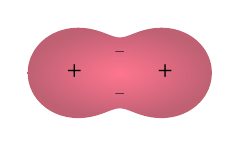
\begin{tikzpicture}[scale=1.8]
			\path[inner color=red4,outer color=red4!70!pag]
			plot[smooth cycle,samples at={0,5,...,360}]
			(  \x:{0.5*(0.9+0.4*cos(2*\x))}  );
			\node at (0.32,0.01) {\small +};
			\node at (-0.32,0.01) {\small +};
			\node at (0,0.15) {\tiny $-$};
			\node at (0,-0.15) {\tiny $-$};

		\end{tikzpicture}                                                                                                                 & Covalent                 & \textcolor{pag!40}{nuceli --- shared e$^{-}$ pair}    & 150 - 1100               & H --- H\TBstrut                                                 \\
		\cline{1-1}
		\multicolumn{5}{c}{\hspace{50pt}$\underline{\textbf{Inter-Particle Forces}}$} \TBstrutfour                                                                                                                                                                                                                        \\
		\cline{1-1}
		% Insert your TikZ diagram for Dipole-dipole here
		\hspace*{-3pt}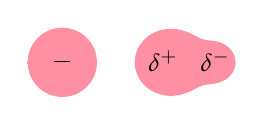
\begin{tikzpicture}[scale=0.8]

			              \path[inner color=red3,outer color=red3,shift={(0,0)}]
			              plot[smooth cycle,samples at={0,5,...,360}]
			              (\x:{1.1*cos(\x)});
			              \node at (0.55,0) {\small $-$};
			              \path[left color=red3,
				              right color=red3,
				              shading angle=90,shift={(2.7,0)}]
			              plot[smooth cycle,samples at={0,5,...,360}]
			              (\x:{0.6+0.2*cos(\x+180)+0.2*cos(2*\x)});
			              \node at (2.98,0.01) {\small $\delta^{-}$};
			              \node at (2.15,0.01) {\small $\delta^{+}$};
		              \end{tikzpicture}                                                                                           & Ion Dipole               & \textcolor{pag!40}{ion charge --- dipole charge}      & 40 - 600                 & Na$^{+}$Cl$^{-}_{(aq)}$ \TTTBBBstrut                                    \\
		% Insert your TikZ diagram for H-bond here
		\hspace*{-2.5pt}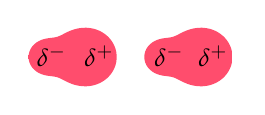
\begin{tikzpicture}[scale=0.7]

			                \path[left color=red5,
				                right color=red5,
				                shading angle=90,shift={(0,0)}]
			                plot[smooth cycle,samples at={0,5,...,360}]
			                (\x:{0.6+0.2*cos(\x)+0.2*cos(2*\x)});
			                \node at (0.68,0.01) {\small $\delta^{+}$};
			                \node at (-0.18,0.01) {\small $\delta^{-}$};

			                \path[left color=red5,
				                right color=red5,
				                shading angle=90,shift={(2.1,0)}]
			                plot[smooth cycle,samples at={0,5,...,360}]
			                (\x:{0.6+0.2*cos(\x)+0.2*cos(2*\x)});
			                \node at (2.75,0.01) {\small $\delta^{+}$};
			                \node at (1.95,0.01) {\small $\delta^{-}$};

		                \end{tikzpicture}                                                                                                           & Dipole Dipole            & \textcolor{pag!40}{dipole charge --- dipole charge}   & 5 - 25                   & NO$_{(g)}$ \TTTBBBstrut                               \\
		% Insert your TikZ diagram for Ion-induced dipole here
		\hspace{3pt}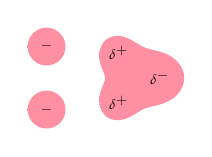
\begin{tikzpicture}[scale=0.8]

			            \path[inner color=red3,outer color=red3,shift={(0.8,-0.5)}]
			            plot[smooth cycle,samples at={0,5,...,360}]
			            (\x:{0.3*cos(\x)^(0)});
			            \node at (0.8,-0.51) {\tiny $-$};

			            \path[inner color=red3,outer color=red3,shift={(0.8,0.5)}]
			            plot[smooth cycle,samples at={0,5,...,360}]
			            (\x:{0.3*cos(\x)^(0)});
			            \node at (0.8,0.51) {\tiny $-$};

			            \path[left color=red3,
				            right color=red3,
				            shading angle=90,shift={(2.1,0)}] plot[smooth cycle,samples at={0,5,...,360}](\x:{( 0.4*(-1.57+ (0.3*(cos(\x)) ) +(0.34*(cos(3*\x))) ))});
			            \node at (1.95,0.4) {\tiny $\delta^{\tiny+}$};
			            \node at (1.95,-0.4) {\tiny $\delta^{\tiny+}$};
			            \node at (2.6,0.01) {\tiny$\delta^{-}$};

		            \end{tikzpicture} & Hydrogen Bonding         & \textcolor{pag!40}{hydrogen dipole --- charge}        & 10 - 40                  & H$_2$O \TBstruttwo                                                                                                                                    \\
		% Insert your TikZ diagram for Dipole-induced dipole here
		\hspace*{-2pt}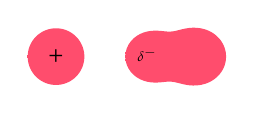
\begin{tikzpicture}[scale=0.8]

			              \path[inner color=red5,outer color=red5,shift={(0,0)}]
			              plot[smooth cycle,samples at={0,5,...,360}]
			              (\x:{0.9*cos(\x)});
			              \node at (0.45,0) {\small +};
			              \path[left color=red5,
				              right color=red5,
				              shading angle=90,shift={(2.3,0)}]
			              plot[smooth cycle,samples at={0,5,...,360}]
			              (\x:{0.6+0.05*cos(\x)+0.2*cos(2*\x)});
			              \node at (1.9,0.02) {\tiny$\delta^{-}$};
		              \end{tikzpicture}                                                                                           & Ion-Induced Dipole       & \textcolor{pag!40}{ion charge --- induced dipole}     & 3 - 15                   & Fe$^{2+}$ --- $\:\:$O$_2$ \TTTBBBstrut                                  \\
		% Insert your TikZ diagram for London dispersion here
		\hspace*{-2.8pt}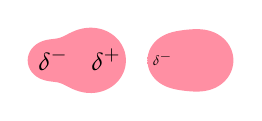
\begin{tikzpicture}[scale=0.78]

			                \path[left color=red3,
				                right color=red3,
				                shading angle=90,shift={(0,0)}]
			                plot[smooth cycle,samples at={0,5,...,360}]
			                (\x:{0.6+0.2*cos(\x)+0.2*cos(2*\x)});
			                \node at (0.68,0.01) {\small $\delta^{+}$};
			                \node at (-0.18,0.01) {\small $\delta^{-}$};

			                \path[left color=red3,
				                right color=red3,
				                shading angle=90,shift={(2,0)}]
			                plot[smooth cycle,samples at={0,5,...,360}]
			                (\x:{0.6+0.05*cos(\x)+0.1*cos(2*\x)});
			                \node at (1.6,0.02) {\tiny$\delta^{-}$};
		                \end{tikzpicture}                                                                                                           & Dipole-Induced Dipole    & \textcolor{pag!40}{dipole charge --- induced dipole}  & 2 - 10                   & O$_2$ --- H$_2$O \TTTBBBstrut                         \\
		\hspace*{-1.5pt}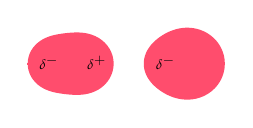
\begin{tikzpicture}[scale=0.78]

			                \path[left color=red5,
				                right color=red5,
				                shading angle=90,
				                shift={(0,0)}]
			                plot[smooth cycle,samples at={0,5,...,360}]
			                (\x:{0.6+0.05*cos(\x)+0.1*cos(2*\x)});
			                \node at (0.48,0.01) {\tiny $\delta^{+}$};
			                \node at (-0.3,0.01) {\tiny $\delta^{-}$};

			                \path[shift={(1.7,0)},
				                left color=red5,
				                right color=red5,
				                shading angle=90]
			                plot[smooth cycle, samples at={0,5,...,360}] (\x:{0.6+0.2*cos(\x)+0.06*cos(2*\x)});
			                \node at (1.6,0.02) {\tiny$\delta^{-}$};
		                \end{tikzpicture}                                                                         & London Dispersion Forces & \textcolor{pag!40}{induced dipole --- induced dipole} & 0.05 - 40                & CCl$_4$ \TTTBBBstrut                                                                    \\
		\cline{1-1}
	\end{tabular}
\end{table}

\pagebreak

\noindent\textbf{Coulomb's Law} - To explain the inter particle forces in more depth, we need to recall Colulomb's Law, which explains the relationship of the attractive force between to charges, to there magnitudes and distance.
\begin{qq}

	\begin{center}
		$F \:\: \propto \:\: \frac{q_1q_2}{r^2} \qquad r=\text{radial distance}\qquad \text{charge}$
	\end{center}

\end{qq}
\vspace{10pt}

\noindent\textbf{Ion-Dipole Forces} - These are very prevalent in solutions. Hydrogen bonding is the most power ion-dipole force, and in solutions, water rips apart ionic compounds and forms a network like structure throughout the solution, where each ion is surrounded by water molecules. The more distributed this is, the more stable the solution.\\
\\
\textbf{Dipole-Dipole Forces} - In dipole-dipole forces, the molecules are lined up to orient there there negative and positive dipole ends forming a bond. Hydrogen bonding is a special case of this, providing a the strongest dipole-dipole bond possible.\\

\hspace{-14pt}\begin{minipage}{0.41\textwidth}

	\textbf{Hydrogen Bonding} - Its important to note that hydrogen bonding will only occur when the atom bonding to the hydrogen \textbf{has a lone pair}, and \textbf{is of similar size}. The large electronegativity difference between the some element and hydrogen leads to a highly polar bond (H$_2$), HF, NH$_3$). In the graph to the right, based on the trend, we would expect water to have a low boiling point, but because of the similar size of hydrogen and oxygen (and the other period 2 elements), the boiling point shoots up.

\end{minipage}
\begin{minipage}[c]{0.6\textwidth}
	\centering
	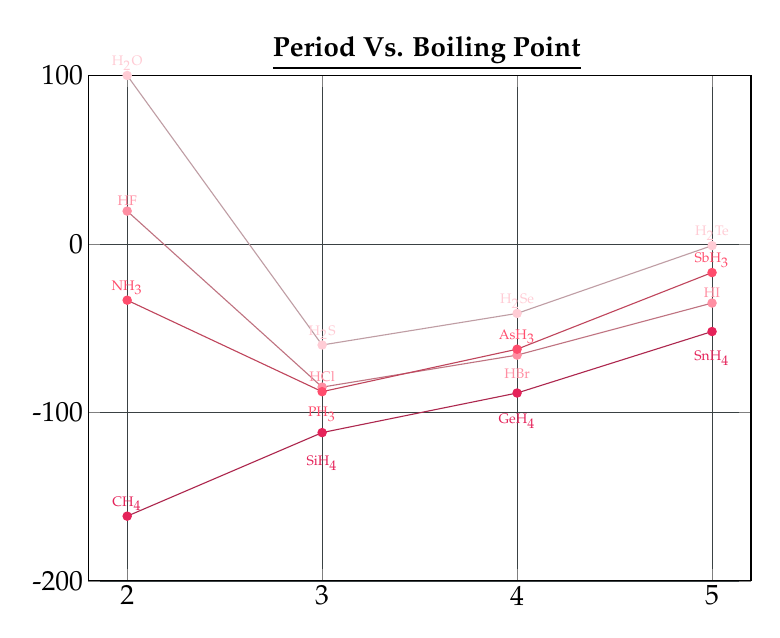
\begin{tikzpicture}

		\begin{axis}[
				xmin=1.8,xmax=5.2,
				ymin=-200,ymax=100,ytick={-200,-100,0,100},
				yticklabels={\normalsize-200,\normalsize-100,\normalsize0,\normalsize100},
				xtick={2,3,4,5},
				xticklabels={\normalsize2, \normalsize3, \normalsize4, \normalsize5},
				major grid style={line width=.2pt,draw=pag!92},
				grid=both,
				width=10cm,
				height=8cm
			]
			\tiny

			\addplot[color=red1!70!pag,no markers] coordinates {(2,100) (3, -60) (4, -41.25) (5, -1)};
			\addplot[
				red1,
				mark=*,
				mark size=1.5pt,
				only marks,
				nodes near coords,
				point meta=explicit symbolic,
			] table [meta=label] {
					x   y      label
					2   100    H$_2$O
					3   -60    H$_2$S
					4   -41.25 H$_2$Se
					5   -1     H$_2$Te
				};

			\addplot[color=red3!70!pag,no markers] coordinates{(2,19.5) (3, -85) (4, -66) (5, -35.1)};
			\addplot[
				red3,
				mark=*,
				mark size=1.5pt,
				only marks,
				nodes near coords,
				point meta=explicit symbolic,
			] table [meta=label] {
					x   y     label
					2   19.5  HF
					3	-85   HCl
					4   -66   \empty
					5   -35.1 HI
				};
			\addplot[red5] coordinates {(3,-101)} node {PH$_3$};
			\addplot[red12] coordinates {(3, -130 )} node {\textcolor{red12}{SiH$_4$}};
			\addplot[color=red5!70!pag,no markers] coordinates{(2,-33.4) (3, -87.7) (4, -62.5) (5, -17)};
			\addplot[
				red5,
				mark=*,
				mark size=1.5pt,
				only marks,
				nodes near coords,
				point meta=explicit symbolic,
			] table [meta=label] {
					x   y     label
					2   -33.4 NH$_3$
					3	-87.7 \empty
					4   -62.5 AsH$_3$
					5   -17   SbH$_3$
				};
			\addplot[red3] coordinates {(4,-77)} node { HBr};

			\addplot[color=red12!70!pag,no markers] coordinates{(2,-161.6) (3, -112) (4, -88.5) (5, -52)};
			\addplot[
				red12,
				mark=*,
				mark size=1.5pt,
				only marks,
				nodes near coords,
				point meta=explicit symbolic,
			] table [meta=label] {
					x   y     label
					2   -161.6 CH$_4$
					3	-112	\empty
					4   -88.5  \empty
					5   -52   \empty
				};
			\addplot[red12] coordinates {(4, -105  )} node {\textcolor{red12}{GeH$_4$}};
			\addplot[red12] coordinates {(5, -68  )} node {\textcolor{red12}{SnH$_4$}};

		\end{axis}
		\node[] at (4.3,6.7) {$\underline{\textbf{Period Vs. Boiling Point}}$};
	\end{tikzpicture}
\end{minipage}

\vspace{10pt}
\noindent \textbf{Ion Induced Dipoles} - When you have an ion, or permanent charge, it can actually shift the electron density of a molecule towards itself creating a temporary dipole in that molecule. An example of this would be iron (Fe$^{2+}$) in hemoglobin (in a porphyrin ring) and oxygen (O$_{2}$). The positive iron pulls on the balanced charge in oxygen, giving it a temporary dipole.\\
\\
\textbf{Dipole-Induced Dipoles} - This is the same as ion induced dipoles, except the rather then a free ion inducing a dipole, a molecule with a preexisting dipole induces another dipole on a different molecule. An example of this would be oxygen dissolved in water, where they hydrogen bonding dipoles of water pull on the electron density of oxygen in the same fashion as the last example.\\
\\
\textbf{Dispersion Forces} - Dispersion forces, or London Forces, are very weak. A molecule in motion will actually have there electron density in a sort of oscillation, moving back and forth. This motion creates temporary dipoles. Eventually, in large quantities, these forces will synchronize with each other, creating a overall force that is not totally negligible.  A good analogy would be metronomes on a table eventually syncing up. Carbon Tetrachloride is an example of this, where the effect of these oscillations are cumulative enough to make its boiling point close to that of water. The greater the strength of the bonds in a molecule, the less freely its density can move, making it more subject to dispersion forces.\\
\\
\pagebreak

\noindent\textbf{Polarizability} - This describes the extent to which the electron density in a molecule can shift within an atom. This relates to all induced dipole interactions. This increases with electron count and molecular size. Its \textit{not} electronegativity, but it follows the exact same trend, just inverse. Also, \textbf{anions} are more polarize then \textbf{cations}.\\
\vspace{-10pt}
\section*{\LARGE\uline{Liquids}}
\newcommand{\randomnessfactor}{0.05}

\begin{minipage}{10cm}
	\textbf{Liquids Definition} - Although we know lots about gases, liquids are poorly understood. The actual physical effects they have are not calculable like gases are. There properties depend on the strengths of inter molecular forces. They have a definite volume, but are not confined to the shape of there container.
\end{minipage}
\begin{minipage}{5cm}
	\tdplotsetmaincoords{70}{165}
	\hspace{5pt}\begin{tikzpicture}
		[tdplot_main_coords,
			grid/.style={very thin,gray},
			axis/.style={->,blue,thick},
			cube/.style={opacity=.5,very thick,},scale=2]
		% draw a grid in the x-y plane
		\foreach \x in {1,1.5,...,3.5}
		\foreach \y in {1,1.5,...,3.5}
			{
				\draw[grid] (\x,1) -- (\x,3.5);
				\draw[grid] (1,\y) -- (3.5,\y);
			}
		% draw the bottom of the cube
		\draw[cube,fill=pag!80,thin] (1.5,1.5,0) -- (1.5,3,0) -- (3,3,0) -- (3,1.5,0) -- cycle;

		% draw the back-right of the cube
		\draw[cube,fill=pag!80,thin] (1.5,1.5,0) -- (1.5,3,0) -- (1.5,3,0.75) -- (1.5,1.5,0.75) -- cycle;

		% draw the back-left of the cube
		\draw[cube,fill=pag!80,thin] (1.5,1.5,0) -- (3,1.5,0) -- (3,1.5,0.75) -- (1.5,1.5,0.75) -- cycle;

		\foreach \z in {0,0.1,...,0.45}
		\foreach \x in {1.6,1.65,...,2.9}
		\foreach \y in {1.6,1.65,...,2.9}{\pgfmathsetmacro{\myangle}{360*rnd}
				\pic at ({\x+(\randomnessfactor*rand)},{\y+(\randomnessfactor*rand)},{0.05+\z+(0.05*rand/2)}) {threedballsthree}; }

		\foreach \z in {0,0.025,...,0.5}
		\foreach \x in {1.6,1.65,...,2.9}
		\foreach \y in {2.9}{\pgfmathsetmacro{\myangle}{360*rnd}
				\pic at ({\x+(\randomnessfactor*rand)},{\y},{0.05+\z+(0.05*rand)}) {threedballsthree}; }
		% draw the axes
		\foreach \z in {0,0.025,...,0.45}
		\foreach \x in {2.9}
		\foreach \y in {1.6,1.7,...,2.9}{\pgfmathsetmacro{\myangle}{360*rnd}
				\pic at ({\x},{\y+(\randomnessfactor*rand)},{0.05+\z+(0.05*rand)}) {threedballsthree}; }

		\foreach \z in {0.5}
		\foreach \x in {1.6,1.65,...,2.9}
		\foreach \y in {1.6,1.65,...,2.9}{\pgfmathsetmacro{\myangle}{360*rnd}
				\pic at ({\x+(\randomnessfactor*rand)},{\y+(\randomnessfactor*rand)},{\z}) {threedballsthree}; }

		% draw the front-right of the cube
		% draw the front-right of the cube
		\draw[cube,thin] (3,1.5,0) -- (3,3,0) -- (3,3,0.75) -- (3,1.5,0.75) -- cycle;

		% draw the front-left of the cube
		\draw[cube,thin] (1.5,3,0) -- (3,3,0) -- (3,3,0.75) -- (1.5,3,0.75) -- cycle;

		% draw the top of the cube
		\draw[cube,thin] (1.5,1.5,0.75) -- (1.5,3,0.75) -- (3,3,0.75) -- (3,1.5,0.75) -- cycle;

	\end{tikzpicture}

\end{minipage}

\vspace{20pt}
\noindent\textbf{Surface Tension} - The official definition says surface tension refers to the resistance of a liquid to increase its surface area. One way to think about it is in terms of liquid droplets. If you spread the liquid into the air, forming droplets, the each droplet will have forces pulling the outer molecules towards the center, as that is where its most stable (most balanced interparticle forces). In the diagrams below, the low surface tension obviously has more surface area. The stronger intermolecular forces, the stronger the surface tension.

\begin{qq}

	\tdplotsetmaincoords{70}{165}
	\renewcommand{\randomnessfactor}{0.05}
	\begin{minipage}{7.3cm}
		\hspace{5pt}\begin{tikzpicture}
			[tdplot_main_coords,
				grid/.style={very thin,gray},
				axis/.style={->,blue,thick},
				cube/.style={opacity=.5,very thick,},scale=2]
			\tikzset{threedballsfive/.pic={
						\foreach \x in {1,2,...,10}{
								% Convert from spherical to Cartesian coordinates
								\pgfmathsetmacro{\theta}{rand*180} % Angle in the xy-plane
								\pgfmathsetmacro{\phi}{rand*360}   % Angle from the z-axis
								\pgfmathsetmacro{\radius}{sqrt((0.01*(rand))+0.01)} % Radius (adjusted for random spread)

								% Spherical to Cartesian conversion formulas
								\pgfmathsetmacro{\xcoord}{\radius*sin(\theta)*cos(\phi)}
								\pgfmathsetmacro{\ycoord}{\radius*sin(\theta)*sin(\phi)}
								\pgfmathsetmacro{\zcoord}{\radius*cos(\theta)}

								\pgfmathsetmacro{\randomIntensity}{random(3,5)} % Generates a random number between 3 and 5
								\fill [color=red\randomIntensity] (\xcoord,\ycoord,\zcoord) circle (0.05cm);
							}
					}}
			% draw a grid in the x-y plane
			\foreach \x in {1,1.5,...,3.5}
			\foreach \y in {1,1.5,...,3.5}
				{
					\draw[grid] (\x,1) -- (\x,3.5);
					\draw[grid] (1,\y) -- (3.5,\y);
				}
			% draw the bottom of the cube
			\draw[cube,fill=pag!80,thin] (1.5,1.5,0) -- (1.5,3,0) -- (3,3,0) -- (3,1.5,0) -- cycle;

			% draw the back-right of the cube
			\draw[cube,fill=pag!80,thin] (1.5,1.5,0) -- (1.5,3,0) -- (1.5,3,2) -- (1.5,1.5,2) -- cycle;

			% draw the back-left of the cube
			\draw[cube,fill=pag!80,thin] (1.5,1.5,0) -- (3,1.5,0) -- (3,1.5,2) -- (1.5,1.5,2) -- cycle;

			\foreach \z in {1,1.5}
			\foreach \x in {1.8,2.25,2.8}
			\foreach \y in {1.8,2.25,2.8}{\pgfmathsetmacro{\myangle}{360*rnd}
					\pic at ({\x+(0.3*rand)},{\y+(0.3*rand)},{0.03+\z+(0.05*rand/2)}) {threedballsfive}; }
			\foreach \z in {0,0.1,...,0.45}
			\foreach \x in {1.6,1.65,...,2.9}
			\foreach \y in {1.6,1.65,...,2.9}{\pgfmathsetmacro{\myangle}{360*rnd}
					\pic at ({\x+(\randomnessfactor*rand)},{\y+(\randomnessfactor*rand)},{0.05+\z+(0.05*rand/2)}) {threedballsthree}; }

			\foreach \z in {0,0.025,...,0.5}
			\foreach \x in {1.6,1.65,...,2.9}
			\foreach \y in {2.9}{\pgfmathsetmacro{\myangle}{360*rnd}
					\pic at ({\x+(\randomnessfactor*rand)},{\y},{0.05+\z+(0.05*rand)}) {threedballsthree}; }
			% draw the axes
			\foreach \z in {0,0.025,...,0.45}
			\foreach \x in {2.9}
			\foreach \y in {1.6,1.7,...,2.9}{\pgfmathsetmacro{\myangle}{360*rnd}
					\pic at ({\x},{\y+(\randomnessfactor*rand)},{0.05+\z+(0.05*rand)}) {threedballsthree}; }

			\foreach \z in {0.5}
			\foreach \x in {1.6,1.65,...,2.9}
			\foreach \y in {1.6,1.65,...,2.9}{\pgfmathsetmacro{\myangle}{360*rnd}
					\pic at ({\x+(\randomnessfactor*rand)},{\y+(\randomnessfactor*rand)},{\z}) {threedballsthree}; }

			\draw[cube,thin] (3,1.5,0) -- (3,3,0) -- (3,3,2) -- (3,1.5,2) -- cycle;

			% draw the front-left of the cube
			\draw[cube,thin] (1.5,3,0) -- (3,3,0) -- (3,3,2) -- (1.5,3,2) -- cycle;

			% draw the top of the cube
			\draw[cube,thin] (1.5,1.5,2) -- (1.5,3,2) -- (3,3,2) -- (3,1.5,2) -- cycle;

		\end{tikzpicture}
	\end{minipage}
	\hspace{5pt}\begin{minipage}{3cm}
		\vspace{9.5pt}
		\begin{tikzpicture}
			[tdplot_main_coords,
				grid/.style={very thin,gray},
				axis/.style={->,blue,thick},
				cube/.style={opacity=.5,very thick,},scale=2]
			\tikzset{threedballssix/.pic={
						\foreach \x in {1,2,...,600}{
								% Convert from spherical to Cartesian coordinates
								\pgfmathsetmacro{\theta}{rand*180} % Angle in the xy-plane
								\pgfmathsetmacro{\phi}{rand*360}   % Angle from the z-axis
								\pgfmathsetmacro{\radius}{sqrt(rand+1)} % Radius (adjusted for random spread)

								% Spherical to Cartesian conversion formulas
								\pgfmathsetmacro{\xcoord}{\radius*sin(\theta)*cos(\phi)}
								\pgfmathsetmacro{\ycoord}{\radius*sin(\theta)*sin(\phi)}
								\pgfmathsetmacro{\zcoord}{\radius*cos(\theta)}

								\pgfmathsetmacro{\randomIntensity}{random(3,5)} % Generates a random number between 3 and 5
								\fill [color=red\randomIntensity] (\xcoord,\ycoord,\zcoord) circle (0.2cm);
							}
					}}

			\foreach \z in {1}
			\foreach \x in {1}
			\foreach \y in {1}{\pgfmathsetmacro{\myangle}{360*rnd}
					\pic at ({\x+(\randomnessfactor*rand)},{\y+(\randomnessfactor*rand)},{0.05+\z+(0.05*rand/2)}) {threedballssix}; }
			\node at (1.25,2,0.2) {$\underline{\text{High Surface Tension}}$};

		\end{tikzpicture}
	\end{minipage}
	\hspace{25pt}\begin{minipage}{3cm}
		\begin{tikzpicture}
			[tdplot_main_coords,
				grid/.style={very thin,gray},
				axis/.style={->,blue,thick},
				cube/.style={opacity=.5,very thick,},scale=2]
			\tikzset{threedballsseven/.pic={
						\foreach \x in {1,2,...,600}{
								% Convert from spherical to Cartesian coordinates
								\pgfmathsetmacro{\theta}{rand*180} % Angle in the xy-plane
								\pgfmathsetmacro{\phi}{rand*360}   % Angle from the z-axis
								\pgfmathsetmacro{\radius}{sqrt(rand+1)} % Radius (adjusted for random spread)

								% Spherical to Cartesian conversion formulas
								\pgfmathsetmacro{\xcoord}{\radius*sin(\theta)*cos(\phi)+(0.7*rand)}
								\pgfmathsetmacro{\ycoord}{\radius*sin(\theta)*sin(\phi)+(0.4*rand)}
								\pgfmathsetmacro{\zcoord}{\radius*cos(\theta)+(0.3*rand)}

								\pgfmathsetmacro{\randomIntensity}{random(3,5)} % Generates a random number between 3 and 5
								\fill [color=red\randomIntensity] (\xcoord,\ycoord,\zcoord) circle (0.2cm);
							}
					}}

			\foreach \z in {1}
			\foreach \x in {1}
			\foreach \y in {1}{\pgfmathsetmacro{\myangle}{360*rnd}
					\pic at ({\x+(\randomnessfactor*rand)},{\y+(\randomnessfactor*rand)},{0.05+\z+(0.05*rand/2)}) {threedballsseven}; }
			\node at (1.2,2,0.2) {$\underline{\text{Low Surface Tension}}$};

		\end{tikzpicture}
	\end{minipage}

\end{qq}

\noindent You can judge the which of two substances has a higher surface tension  by determining the strength of each substances intermolecular forces. Between CH$_3$CH$_2$OH and H$_2$O, water has strong hydrogen bonding, meaning it will have much stronger surface tension.\\
\begin{minipage}{9.5cm}
	\textbf{Capillarity} - This refers to the intermolecular forces between liquid and the surface its in contanct with. This usally only happens in a tube. When we are looking at water in a silicon dioxide tube, its pulled upwards due to hydrogen bonding between the water and the silicon. If the water were replaced with mercery, it would not have enough cumulative inter molecular force to overcome the the cohesive forces, or the forces holding the liquid (mercury) together. A liquid undergoing capillary action in a tube will form a meniscus.

\end{minipage}
\begin{minipage}{5cm}

	\tdplotsetmaincoords{70}{125}
	\hspace{5pt}\begin{tikzpicture}
		[tdplot_main_coords,
			grid/.style={very thin,gray},
			axis/.style={->,blue,thick},
			cube/.style={opacity=.5,very thick,},scale=2]
		% draw a grid in the x-y plane
		\foreach \x in {1,1.5,...,3.5}
		\foreach \y in {1,1.5,...,3.5}
			{
				\draw[grid] (\x,1) -- (\x,3.5);
				\draw[grid] (1,\y) -- (3.5,\y);
			}
		% draw the bottom of the cube
		\draw[cube,thin] (1.5,1.5,0) -- (1.5,3,0) -- (3,3,0) -- (3,1.5,0) -- cycle;

		% draw the back-right of the cube
		\draw[cube,fill=pag!80,thin] (1.5,1.5,0) -- (1.5,3,0) -- (1.5,3,2) -- (1.5,1.5,2) -- cycle;

		% draw the back-left of the cube
		\draw[cube,thin] (1.5,1.5,0) -- (3,1.5,0) -- (3,1.5,2) -- (1.5,1.5,2) -- cycle;

		\foreach \z in {0,0.1,...,0.4}
		\foreach \x in {1.6,1.65,...,2.9}
		\foreach \y in {1.6,1.65,...,2.9}{\pgfmathsetmacro{\myangle}{360*rnd}
				\pic at ({\x+(\randomnessfactor*rand)},{\y+(\randomnessfactor*rand)},{0.05+\z+(0.05*rand/2)}) {threedballsthree}; }

		\foreach \z in {0,0.025,...,0.5}
		\foreach \x in {1.6,1.65,...,2.9}
		\foreach \y in {2.9}{\pgfmathsetmacro{\myangle}{360*rnd}
				\pic at ({\x+(\randomnessfactor*rand)},{\y},{0.05+\z+(0.05*rand)}) {threedballsthree}; }
		% draw the axes
		\foreach \z in {0,0.025,...,0.5}
		\foreach \x in {2.9}
		\foreach \y in {1.6,1.7,...,2.9}{\pgfmathsetmacro{\myangle}{360*rnd}
				\pic at ({\x},{\y+(\randomnessfactor*rand)},{0.05+\z+(0.05*rand)}) {threedballsthree}; }

		\foreach \z in {0.4,0.425,...,1.2}
		\foreach \x in {1.6}
		\foreach \y in {1.6,1.7,...,2.9}{\pgfmathsetmacro{\myangle}{360*rnd}
				\pic at ({\x},{\y+(\randomnessfactor*rand)},{0.05+\z+(0.05*rand)}) {threedballsthree}; }

		\foreach \z in {0.5}
		\foreach \x in {1.6,1.65,...,2.9}
		\foreach \y in {1.6,1.65,...,2.9}{\pgfmathsetmacro{\myangle}{360*rnd}
				\pic at ({\x+(\randomnessfactor*rand)},{\y+(\randomnessfactor*rand)},{\z}) {threedballsthree}; }

		% draw the front-right of the cube
		% draw the front-right of the cube
		\draw[cube,thin] (3,1.5,0) -- (3,3,0) -- (3,3,2) -- (3,1.5,2) -- cycle;

		% draw the front-left of the cube
		\draw[cube,thin] (1.5,3,0) -- (3,3,0) -- (3,3,2) -- (1.5,3,2) -- cycle;

		% draw the top of the cube
		\draw[cube,thin] (1.5,1.5,2) -- (1.5,3,2) -- (3,3,2) -- (3,1.5,2) -- cycle;

	\end{tikzpicture}

\end{minipage}

\pagebreak

\noindent One more example of capillarity can be seen in water versus hexane on a glass surface. The water, being attracted to the surface of the glass, will spread itself out, where as the hexane will clump together in a similar way to a droplet. There are no forces pulling the hexane towards the surface, so there is no way for it to resist its surface tension.
\begin{qq}

	\begin{center}
		\hspace*{-8pt}\begin{minipage}{7cm}
			\hspace{5pt}\begin{tikzpicture}
				[tdplot_main_coords,
					grid/.style={very thin,gray},
					axis/.style={->,blue,thick},
					cube/.style={opacity=.5,very thick,},scale=2]
				\tikzset{threedballsfive/.pic={
							\foreach \x in {1,2,...,20}{
									% Convert from spherical to Cartesian coordinates
									\pgfmathsetmacro{\theta}{rand*180} % Angle in the xy-plane
									\pgfmathsetmacro{\phi}{rand*360}   % Angle from the z-axis
									\pgfmathsetmacro{\radius}{sqrt((0.01*(rand))+0.01)} % Radius (adjusted for random spread)

									% Spherical to Cartesian conversion formulas
									\pgfmathsetmacro{\xcoord}{\radius*sin(\theta)*cos(\phi)}
									\pgfmathsetmacro{\ycoord}{\radius*sin(\theta)*sin(\phi)}
									\pgfmathsetmacro{\zcoord}{\radius*cos(\theta)}

									\pgfmathsetmacro{\randomIntensity}{random(3,5)} % Generates a random number between 3 and 5
									\fill [color=red\randomIntensity] (\xcoord,\ycoord,\zcoord) circle (0.05cm);
								}
						}}
				% draw a grid in the x-y plane
				\foreach \x in {1,1.5,...,3.5}
				\foreach \y in {1,1.5,...,3.5}
					{
						\draw[grid] (\x,1) -- (\x,3.5);
						\draw[grid] (1,\y) -- (3.5,\y);
					}
				% draw the bottom of the cube
				\draw[cube,fill=pag!80,thin] (1.5,1.5,0) -- (1.5,3,0) -- (3,3,0) -- (3,1.5,0) -- cycle;

				% draw the back-right of the cube
				\draw[cube,fill=pag!80,thin] (1.5,1.5,0) -- (1.5,3,0) -- (1.5,3,0.25) -- (1.5,1.5,0.25) -- cycle;

				% draw the back-left of the cube
				\draw[cube,fill=pag!80,thin] (1.5,1.5,0) -- (3,1.5,0) -- (3,1.5,0.25) -- (1.5,1.5,0.25) -- cycle;

				% draw the axes

				\draw[cube,fill=pag!80,thin] (3,1.5,0) -- (3,3,0) -- (3,3,0.25) -- (3,1.5,0.25) -- cycle;

				% draw the front-left of the cube
				\draw[cube,fill=pag!80,thin] (1.5,3,0) -- (3,3,0) -- (3,3,0.25) -- (1.5,3,0.25) -- cycle;

				% draw the top of the cube
				\draw[cube,fill=pag!80,thin] (1.5,1.5,0.25) -- (1.5,3,0.25) -- (3,3,0.25) -- (3,1.5,0.25) -- cycle;

				\foreach \z in {0.2,0.3}
				\foreach \x in {1.7,1.75,...,2.8}
				\foreach \y in {1.7,1.75,...,2.8}{\pgfmathsetmacro{\myangle}{360*rnd}
						\pic at ({\x+(\randomnessfactor*rand)},{\y+(\randomnessfactor*rand)},{0.05+\z+(0.05*rand/2)}) {threedballsthree}; }

			\end{tikzpicture}
			\begin{center}
				$\quad\:\:\underline{\text{Water}}$
			\end{center}
		\end{minipage}
		\hspace{20pt}\begin{minipage}{7cm}
			\hspace{5pt}\begin{tikzpicture}
				[tdplot_main_coords,
					grid/.style={very thin,gray},
					axis/.style={->,blue,thick},
					cube/.style={opacity=.5,very thick,},scale=2]
				\tikzset{threedballsnine/.pic={
							\foreach \x in {1,2,...,50}{
									% Convert from spherical to Cartesian coordinates
									\pgfmathsetmacro{\theta}{rand*180} % Angle in the xy-plane
									\pgfmathsetmacro{\phi}{rand*360}   % Angle from the z-axis
									\pgfmathsetmacro{\radius}{sqrt((0.01*(rand))+0.01)} % Radius (adjusted for random spread)

									% Spherical to Cartesian conversion formulas
									\pgfmathsetmacro{\xcoord}{\radius*sin(\theta)*cos(\phi)}
									\pgfmathsetmacro{\ycoord}{\radius*sin(\theta)*sin(\phi)}
									\pgfmathsetmacro{\zcoord}{\radius*cos(\theta)}

									\pgfmathsetmacro{\randomIntensity}{random(3,5)} % Generates a random number between 3 and 5
									\fill [color=red\randomIntensity] (\xcoord,\ycoord,\zcoord) circle (0.05cm);
								}
						}}
				% draw a grid in the x-y plane
				\foreach \x in {1,1.5,...,3.5}
				\foreach \y in {1,1.5,...,3.5}
					{
						\draw[grid] (\x,1) -- (\x,3.5);
						\draw[grid] (1,\y) -- (3.5,\y);
					}
				% draw the bottom of the cube
				\draw[cube,fill=pag!80,thin] (1.5,1.5,0) -- (1.5,3,0) -- (3,3,0) -- (3,1.5,0) -- cycle;

				% draw the back-right of the cube
				\draw[cube,fill=pag!80,thin] (1.5,1.5,0) -- (1.5,3,0) -- (1.5,3,0.25) -- (1.5,1.5,0.25) -- cycle;

				% draw the back-left of the cube
				\draw[cube,fill=pag!80,thin] (1.5,1.5,0) -- (3,1.5,0) -- (3,1.5,0.25) -- (1.5,1.5,0.25) -- cycle;

				% draw the axes

				\draw[cube,fill=pag!80,thin] (3,1.5,0) -- (3,3,0) -- (3,3,0.25) -- (3,1.5,0.25) -- cycle;

				% draw the front-left of the cube
				\draw[cube,fill=pag!80,thin] (1.5,3,0) -- (3,3,0) -- (3,3,0.25) -- (1.5,3,0.25) -- cycle;

				% draw the top of the cube
				\draw[cube,fill=pag!80,thin] (1.5,1.5,0.25) -- (1.5,3,0.25) -- (3,3,0.25) -- (3,1.5,0.25) -- cycle;

				\foreach \z in {0.3}
				\foreach \x in {1.7,1.9,...,2.8}
				\foreach \y in {1.7,1.9,...,2.8}{\pgfmathsetmacro{\myangle}{360*rnd}
						\pic at ({\x+(0.1*rand)},{\y+(0.1*rand)},{\z}) {threedballsnine}; }
			\end{tikzpicture}
			\begin{center}
				$\quad\:\:\underline{\text{Hexan}}$
			\end{center}
		\end{minipage}

	\end{center}

\end{qq}
\noindent For a \textbf{polyvinyl acetate} surface, the opposite would occur. This is because the Hexane can participate in dispersion forces with the surface. \\
\\
\textbf{Viscosity} - Viscosity refers to a liquids resistance to flow. High viscosity substances like honey imply strong intermolecular forces. \\
\\
\textbf{Motor Oils } - Motor oils specifically, made of long hydrocarbon chains, are special as they need to maintain a level of viscosity throughout a range of temperatures. In the cold, they need to be fluid enough for your engine to run. Once the engine is running, it will be very hot, so the oil must be viscous enough to maintain lubrication. The long longer a hydrocarbon chain the stronger the dispersion forces, and subsequently the stronger the viscosity. In low temperatures, the hydrocarbon chains fold into each other, causing far less dispersion forces then the long chains found at warmer temperatures.\\
\\
\textbf{Solubility} - A solution is a homogeneous mixture in which the solute is dissolved in the solvent. The substances a solution can be composed of are not limited to water. In general however, the rule \textbf{like dissolves like} applies when trying to determine solubility. This basically says that the interparticle forces in the solute and the solvent are similar, then the solubility will be favored.\\
\\
An example of this is polystyrene in water versus acetone. Polystyrene is a very non-polar molecule being a long chain of carbon bounded to hydrogen and benzene rings. In water, it won't dissolve due to waters strong polarity. In something like acetone (on the left), it will dissolve, as acetone is similar in that it is relatively non polar. It also has dispersion forces like the long chain.

\begin{qq}

	\begin{center}

		\hspace{-10pt}\begin{minipage}{10cm}

			\scalebox{0.5}{\chemfig{C(-[:90]*6(=-=-=-))(-[6]H)-C(-[2]H)(-[6]H)-[@{right,0.8}]C(-[:90]*6(=-=-=-))(-[6]H)-C(-[2]H)(-[6]H)-[@{right,0.8}]C(-[:90]*6(=-=-=-))(-[6]H)-C(-[2]H)(-[6]H)-[@{right,0.8}]C(-[:90]*6(=-=-=-))(-[6]H)-C(-[2]H)(-[6]H)-[@{right,0.8}]C(-[:90]*6(=-=-=-))(-[6]H)-C(-[2]H)(-[6]H)-[@{right,0.8}]C(-[:90]*6(=-=-=-))(-[6]H)-C(-[2]H)(-[6]H)-[@{right,0.8}]C(-[:90]*6(=-=-=-))(-[6]H)-C(-[2]H)(-[6]H)-[@{right,0.8}]C(-[:90]*6(=-=-=-))(-[6]H)-C(-[2]H)(-[6]H)-[@{right,0.8}]C(-[:90]*6(=-=-=-))(-[6]H)}}
		\end{minipage}
		\hspace{20pt}\begin{minipage}{3cm}

			\scalebox{0.8}{\chemfig{O(=[:270]C(-[:330]C(-[:20]H)(-[:315]H)(-[:240]H) )(-[:210]C(-[:160]H)(-[:230]H)(-[:300]H)) )}}

		\end{minipage}
	\end{center}

\end{qq}

\vspace{5pt}
\noindent\begin{minipage}{14cm}
	\vspace{10pt}
	Another example would be Iodine in dichloromethane (CH$_2$Cl$_2$), water, and hexane (C$_6$H$_{14}$). In this case, iodine, being a very non polar molecule, would not dissolve in water. If you set up an experiment using a glass with the three chemicals stacked atop each other (there densities are different, and they are insoluble with each other), iodine would dissolve in the hexane because of hexanes because of hexanes non-polarity. If you pushed the iodine past the hexane, it would fall right through the water until it hits the dicholormethane which it can dissolve with. Dicholormethane does have a small dipole, but it is relatively similar to iodine, so the majorty of the forces are dispersion.
\end{minipage}
\hspace{16.5pt}\begin{minipage}{1cm}

	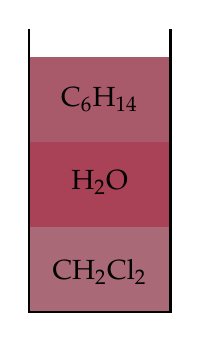
\begin{tikzpicture}[scale=0.6]

		\fill[red3!60!pag] (0,0) rectangle (3,1.8);
		\fill[red5!60!pag] (0,1.8) rectangle (3,3.6);
		\fill[red4!60!pag] (0,3.6) rectangle (3,5.4);

		% Labels, adjust positions as needed
		\node at (1.5, 0.85) {CH$_2$Cl$_2$ };
		\node at (1.5, 2.75) {H\textsubscript{2}O};
		\node at (1.5, 4.5) {C$_6$H$_{14}$};

		\draw[thick] (0,6) -- (0,0) -- (3,0) -- (3,6);
	\end{tikzpicture}
\end{minipage}

\pagebreak

\noindent\textbf{Alkanes and Water} - A solution of water and some alkane will never happen. Alkanes only undergo dispersion forces, while water has strong hydrogen bonding. The dispersion forces of some alkane are not strong enough to overcome the hydrogen bonding of the water. On the interface between the two, the alkane will experience dipole induced dipole forces.\\
\\
\textbf{Salt's and Water} - As discussed previously, a salt in water will be torn apart by the cumulative effect of the waters hydrogen bonding to the ionic charges will overcome the two substances individual interparticle forces (waters hydrogen bonding and the salts ionic bonding).\\
\\
\textbf{Cocaine and Water} - Cocaine only has one small dipole on its methane -- nitrogen bond, making it very insoluble in water. To increase cocaine's solubility, we can add hydrochloric acid $HCl$ to the cocaine such that the hydrogen in HCl bonds to the lone pair on cocaine's nitrogen. Extracting the cocaine salt formed leaves us with a form of cocaine that is dissolvable in water.
\begin{qq}

	\begin{center}

		\hspace{20pt}\begin{minipage}{7.2cm}

			\scalebox{0.8}{\chemfig{H_2C(-C?[a]H-[:-30]CH_2-[:30]C?[b]H-O-CO-C_6H_5)
			-[2]CH_2-[,1.7]CH(-[3]N?[a]-[3]H_3C)(-[,1.35]C?[b]H-CO-OCH_3)}}

		\end{minipage}
		\begin{minipage}{7cm}

			\scalebox{0.8}{\chemfig{H_2C(-C?[a]H-[:-30]CH_2-[:30]C?[b]H-O-CO-C_6H_5)
			-[2]CH_2-[,1.7]CH(-[3]N?[a](-[:45]H)-[3]H_3C)(-[,1.35]C?[b]H-CO-OCH_3)}}

		\end{minipage}

	\end{center}

\end{qq}
\section*{\LARGE\uline{Solids}}
\begin{minipage}{10cm}
	\textbf{Solids Definition} - Solids are tightly packed materials with a definite volume shape. The particles are very hard to move. There are two main forms of solids, crystalline and amorphous.
\end{minipage}
\begin{minipage}{5cm}
	\tdplotsetmaincoords{70}{165}
	\hspace{5pt}\begin{tikzpicture}
		[tdplot_main_coords,
			grid/.style={very thin,gray},
			axis/.style={->,blue,thick},
			cube/.style={opacity=.5,very thick,},scale=2]

		\tikzset{threedballseleven/.pic={
					\pgfmathsetmacro{\randomIntensity}{random(3,5)} % Generates a random number between 3 and 6
					\fill [color= red\randomIntensity] (-0.00cm,-0.00cm,0) circle (0.07cm);
				}}
		% draw a grid in the x-y plane
		\foreach \x in {1,1.5,...,3.5}
		\foreach \y in {1,1.5,...,3.5}
			{
				\draw[grid] (\x,1) -- (\x,3.5);
				\draw[grid] (1,\y) -- (3.5,\y);
			}
		% draw the bottom of the cube
		\draw[cube,fill=pag!80,thin] (1.5,1.5,0) -- (1.5,3,0) -- (3,3,0) -- (3,1.5,0) -- cycle;

		% draw the back-right of the cube
		\draw[cube,fill=pag!80,thin] (1.5,1.5,0) -- (1.5,3,0) -- (1.5,3,0.75) -- (1.5,1.5,0.75) -- cycle;

		% draw the back-left of the cube
		\draw[cube,fill=pag!80,thin] (1.5,1.5,0) -- (3,1.5,0) -- (3,1.5,0.75) -- (1.5,1.5,0.75) -- cycle;
		\foreach \z in {0,0.05,...,0.7}
		\foreach \x in {1.56,1.61,...,2.99}
		\foreach \y in {1.56,1.61,...,2.99}{\pgfmathsetmacro{\myangle}{360*rnd}
				\pic at ({\x},{\y},{0.05+\z}) {threedballseleven}; }

		% draw the front-right of the cube
		% draw the front-right of the cube
		\draw[cube,thin] (3,1.5,0) -- (3,3,0) -- (3,3,0.75) -- (3,1.5,0.75) -- cycle;

		% draw the front-left of the cube
		\draw[cube,thin] (1.5,3,0) -- (3,3,0) -- (3,3,0.75) -- (1.5,3,0.75) -- cycle;

		% draw the top of the cube
		\draw[cube,thin] (1.5,1.5,0.75) -- (1.5,3,0.75) -- (3,3,0.75) -- (3,1.5,0.75) -- cycle;

	\end{tikzpicture}

\end{minipage}

\vspace{10pt}
\noindent\textbf{Crystalline Solids} - These end up being the focus for solids in this course. Crystalline solids are network structures with a definite shape. They have a very ordered arrangement. Ice is an example of this. Halite, (predominantly sodium chloride) forms large blocky crystals and are mined to produce table salt. Simple ionic network structures are crystalline too.\\
\\
\textbf{Amorphous} - These are solids that don't have much incentive to form a molecular structure, but still have enough cumulative inter molecular forces to hold themselves together. Plastics and glass are examples of this. The structure of amorphous solids can be analyzed looking at the average of its structure.\\
\\

\newcommand{\Tstrutsolids}{\rule{0pt}{7ex}}         % Top strut
\newcommand{\Bstrutsolids}{\rule[-7ex]{0pt}{0pt}}   % Bottom strut
\newcommand{\TBstrutsolids}{\Tstrutsolids\Bstrutsolids}
\newcommand{\Tstrutsolidstwo}{\rule{0pt}{3ex}}         % Top strut
\newcommand{\Bstrutsolidstwo}{\rule[-1.5ex]{0pt}{0pt}}   % Bottom strut
\newcommand{\TBstrutsolidstwo}{\Tstrutsolidstwo\Bstrutsolidstwo}
\newcommand{\Tstrutsolidsthree}{\rule{0pt}{2.5ex}}         % Top strut
\newcommand{\Bstrutsolidsthree}{\rule[-1ex]{0pt}{0pt}}   % Bottom strut
\newcommand{\TBstrutsolidsthree}{\Tstrutsolidsthree\Bstrutsolidsthree}
\begin{qq}

	\begin{center}

		$\underline{\textbf{Types of Crystalline Solids}}$
		\vspace{3pt}

		\begin{tabular}{clll}
			\hline
			Type                      & Interparticle Force & Physical Properties          & Examples \TBstrutsolidsthree \\
			\hline
			\multicolumn{4}{l}{\textbf{Discrete Molecular Structures}} \TBstrutsolidstwo                                  \\
			\hline
			\textit{Non-Polar}        & Disperson Forces    & \makecell[l]{soft                                           \\ low melting point \\ poor thermal and \\ electrical conductor} & \makecell[l]{CH$_{4(s)}$ \textcolor{pag!60}{(mp: -182$^{\circ}$C)} \\ CO$_{2(s)}$ \textcolor{pag!60}{(mp: -78 $^{\circ}$C)} \\ Ar$_{(s)}$ $\:\:\:\:$\textcolor{pag!60}{(mp: -189 $^{\circ}$C)}} \TBstrutsolids \\

			\makecell[c]{\textit{Polar}                                                                                   \\ \textit{Hydrogen Bonded}}& \makecell{Dipole-Dipole \\ H-Bonding} & \makecell[l]{fairly soft \\ low melting point \\ poor thermal and \\ electrical conductor} &  \makecell[l]{ H$_2$O$_{(s)}$ \textcolor{pag!60}{$\:\:\:\:$(mp: 0$^{\circ}$C)} \\ CHCl$_{3(s)}$ \textcolor{pag!60}{(mp: -64$^{\circ}$C)} }	\TBstrutsolids \\
			\hline
			\multicolumn{4}{l}{\textbf{Extended Structures}}\TBstrutsolidstwo                                             \\
			\hline
			\textit{Ionic}            & Ionic Bonding       & \makecell[l]{hard \& brittle                                \\ high melting point\\ good thermal and \\ electrical conductor} &  \makecell[l]{ CsCl$_{(s)}$ $\:$\textcolor{pag!60}{(mp: 645$^{\circ}$C)} \\ MgO$_{(s)}$ \textcolor{pag!60}{(mp: 2800$^{\circ}$C)} }	\TBstrutsolids \\

			\textit{Covalent Network} & Covalent Bonding    & \makecell[l]{very hard                                      \\ extreme melting point\\ poor thermal* and \\ electrical conductor} &  \makecell[l]{ C$_{(diamond)}$ $\:$\textcolor{pag!60}{(mp: $>$3500$^{\circ}$C)} \\ SiO$_{2(s)}$ $\:\:\:\:\:\:\:$\textcolor{pag!60}{(mp:  1600$^{\circ}$C)} }	\TBstrutsolids \\

			\textit{Metallic}         & Metallic Bonding    & \makecell[l]{soft to hard                                   \\ high melting point\\ lustrous \\ ductile \& malleable \\ excellent thermal and \\ electrical conductor} &  \makecell[l]{ Au$_{(s)}$ $\:$\textcolor{pag!60}{(mp: 1064$^{\circ}$C)} \\ Cu$_{(s)}$ $\:$\textcolor{pag!60}{(mp:  1085$^{\circ}$C)} }	\TBstrutsolids \\
		\end{tabular}
	\end{center}

\end{qq}

\pagebreak

\begin{minipage}{7.75cm}
	\textbf{Lattice} - A lattice is a 3D representation of the arrangement of some crystalline structure. It does not describe what each point in a crystal structure is, but rather the repeating arrangement of these points.
\end{minipage}
\begin{minipage}{4cm}
	\tdplotsetmaincoords{70}{127.5}
	\hspace{5pt}\begin{tikzpicture}
		[tdplot_main_coords,
			grid/.style={very thin,gray},
			axis/.style={->,blue,thick},
			cube/.style={opacity=.6,very thick,},scale=2.5]

		\newcounter{ballCounter}

		\tikzset{
			threedballseleven/.pic={
					% Increment the counter
					\stepcounter{ballCounter}

					% Check if the counter is even or odd
					\pgfmathparse{mod(\theballCounter,2) == 0 ? "pag!70" : "pag!70"}
					\edef\ballColor{\pgfmathresult} % Store the result in \ballColor

					% Use the determined color
					\fill [ball color=\ballColor, color=pag] (-0.00cm,-0.00cm,0) circle (0.125cm);
				}
		}
		\foreach \x [count=\xi] in {0,0.5,1}
		\foreach \z [count=\zi] in {0,0.5,1}
		\foreach \y [count=\yi] in {0,0.5,1}{

				% Draw the circle
				\ifnum\zi<3
					\pgfmathsetmacro{\nextz}{\z+0.5}
					\draw[thick,pag!60] ({\x},{\y},{0.05+\z}) -- ({\x},{\y},{0.05+\nextz});
				\fi

				% Draw horizontal lines to the next circle
				\ifnum\xi<3
					\pgfmathsetmacro{\nextx}{\x+0.5}
					\draw[thick,pag!60] ({\x},{\y},{0.05+\z}) -- ({\nextx},{\y},{0.05+\z});
				\fi

				% Draw vertical lines to the next circle
				\ifnum\yi<3
					\pgfmathsetmacro{\nexty}{\y+0.5}
					\draw[thick,pag!60] ({\x},{\y},{0.05+\z}) -- ({\x},{\nexty},{0.05+\z});
				\fi

				\pgfmathsetmacro{\myangle}{360*rnd}
				\pic at ({\x},{\y},{0.05+\z}) {threedballseleven};

			}

	\end{tikzpicture}
\end{minipage}
\begin{minipage}{5cm}
	\tdplotsetmaincoords{70}{145}
	\hspace{5pt}\begin{tikzpicture}
		[tdplot_main_coords,
			grid/.style={very thin,gray},
			axis/.style={->,blue,thick},
			cube/.style={opacity=.6,very thick,},scale=2.5]

		\newcounter{ballCounter}

		\tikzset{
			threedballseleven/.pic={
					% Increment the counter
					\stepcounter{ballCounter}

					% Check if the counter is even or odd
					\pgfmathparse{mod(\theballCounter,2) == 0 ? "pag!70" : "pag!70"}
					\edef\ballColor{\pgfmathresult} % Store the result in \ballColor

					% Use the determined color
					\fill [ball color=\ballColor, color=pag] (-0.00cm,-0.00cm,0) circle (0.125cm);
				}
		}
		\foreach \x [count=\xi] in {0,0.5,1}
		\foreach \z [count=\zi] in {0,0.5,1}
		\foreach \y [count=\yi] in {0,0.5,1}{

				% Draw the circle
				\ifnum\zi<3
					\pgfmathsetmacro{\nextz}{\z+0.5}
					\draw[thick,pag!60] ({\x},{\y},{0.05+\z}) -- ({\x},{\y},{0.05+\nextz});
				\fi

				% Draw horizontal lines to the next circle
				\ifnum\xi<3
					\pgfmathsetmacro{\nextx}{\x+0.5}
					\draw[thick,pag!60] ({\x},{\y},{0.05+\z}) -- ({\nextx},{\y},{0.05+\z});
				\fi

				% Draw vertical lines to the next circle
				\ifnum\yi<3
					\pgfmathsetmacro{\nexty}{\y+0.5}
					\draw[thick,pag!60] ({\x},{\y},{0.05+\z}) -- ({\x},{\nexty},{0.05+\z});
				\fi

				\pgfmathsetmacro{\myangle}{360*rnd}
				\pic at ({\x},{\y},{0.05+\z}) {threedballseleven};

			}

	\end{tikzpicture}
\end{minipage}

\begin{minipage}{7.75cm}
	\textbf{Unit Cell} - The symmetrical shape of crystalline solids suggests a ordered arrangement of atoms. A unit cell is simply the smallest volume with representative symmetry which when repeated generate the crystal structure.
\end{minipage}
\begin{minipage}{4cm}
	\tdplotsetmaincoords{70}{127.5}
	\hspace{5pt}\begin{tikzpicture}
		[tdplot_main_coords,
			grid/.style={very thin,gray},
			axis/.style={->,blue,thick},
			cube/.style={opacity=.6,very thick,},scale=2.5]

		\newcounter{ballCounter}
		\newcounter{ballCountertwoo}

		\tikzset{
			threedballselevenn/.pic={
					% Increment the counter
					\stepcounter{ballCountertwoo}

					% Check if the counter is even or odd
					\pgfmathparse{mod(\theballCountertwoo,2) == 0 ? "pag!60" : "pag!60"}
					\edef\ballColor{\pgfmathresult} % Store the result in \ballColor

					% Use the determined color
					\fill [ball color=\ballColor, color=pag] (-0.00cm,-0.00cm,0) circle (0.1cm);}}

		\foreach \x [count=\xi] in {0,0.5,1}
		\foreach \z [count=\zi] in {0,0.5,1}
		\foreach \y [count=\yi] in {0,0.5,1}{

				% Draw the circle
				\ifnum\zi<3
					\pgfmathsetmacro{\nextz}{\z+0.5}
					\draw[thick,pag!60] ({\x},{\y},{0.05+\z}) -- ({\x},{\y},{0.05+\nextz});
				\fi

				% Draw horizontal lines to the next circle
				\ifnum\xi<3
					\pgfmathsetmacro{\nextx}{\x+0.5}
					\draw[thick,pag!60] ({\x},{\y},{0.05+\z}) -- ({\nextx},{\y},{0.05+\z});
				\fi

				% Draw vertical lines to the next circle
				\ifnum\yi<3
					\pgfmathsetmacro{\nexty}{\y+0.5}
					\draw[thick,pag!60] ({\x},{\y},{0.05+\z}) -- ({\x},{\nexty},{0.05+\z});
				\fi

				\pgfmathsetmacro{\myangle}{360*rnd}
				\pic at ({\x},{\y},{0.05+\z}) {threedballselevenn};}

		\tikzset{
			threedballseleven/.pic={
					\stepcounter{ballCounter}
					\pgfmathparse{mod(\theballCounter,2) == 0 ? "red4" : "red4"}
					\edef\ballColor{\pgfmathresult}
					\fill [ball color=\ballColor, color=pag] (-0.00cm,-0.00cm,0) circle (0.1cm);}}

		\foreach \x [count=\xi] in {0.5,1}
		\foreach \z [count=\zi] in {0.5,1}
		\foreach \y [count=\yi] in {0.5,1}{

				\ifnum\zi<2
					\pgfmathsetmacro{\nextz}{\z+0.5}
					\draw[thick,pag!60] ({\x},{\y},{0.05+\z}) -- ({\x},{\y},{0.05+\nextz});
				\fi

				\ifnum\xi<2
					\pgfmathsetmacro{\nextx}{\x+0.5}
					\draw[thick,pag!60] ({\x},{\y},{0.05+\z}) -- ({\nextx},{\y},{0.05+\z});
				\fi

				\ifnum\yi<2
					\pgfmathsetmacro{\nexty}{\y+0.5}
					\draw[thick,pag!60] ({\x},{\y},{0.05+\z}) -- ({\x},{\nexty},{0.05+\z});
				\fi

				\pgfmathsetmacro{\myangle}{360*rnd}
				\pic at ({\x},{\y},{0.05+\z}) {threedballseleven};}

	\end{tikzpicture}
\end{minipage}
\begin{minipage}{5cm}

	\tdplotsetmaincoords{70}{145}
	\hspace{5pt}\begin{tikzpicture}
		[tdplot_main_coords,
			grid/.style={very thin,gray},
			axis/.style={->,blue,thick},
			cube/.style={opacity=.6,very thick,},scale=2.5]

		\newcounter{ballCounter}
		\newcounter{ballCountertwoo}

		\tikzset{
			threedballselevenn/.pic={
					% Increment the counter
					\stepcounter{ballCountertwoo}

					% Check if the counter is even or odd
					\pgfmathparse{mod(\theballCountertwoo,2) == 0 ? "pag!60" : "pag!60"}
					\edef\ballColor{\pgfmathresult} % Store the result in \ballColor

					% Use the determined color
					\fill [ball color=\ballColor, color=pag] (-0.00cm,-0.00cm,0) circle (0.1cm);}}

		\foreach \x [count=\xi] in {0,0.5,1}
		\foreach \z [count=\zi] in {0,0.5,1}
		\foreach \y [count=\yi] in {0,0.5,1}{

				% Draw the circle
				\ifnum\zi<3
					\pgfmathsetmacro{\nextz}{\z+0.5}
					\draw[thick,pag!60] ({\x},{\y},{0.05+\z}) -- ({\x},{\y},{0.05+\nextz});
				\fi

				% Draw horizontal lines to the next circle
				\ifnum\xi<3
					\pgfmathsetmacro{\nextx}{\x+0.5}
					\draw[thick,pag!60] ({\x},{\y},{0.05+\z}) -- ({\nextx},{\y},{0.05+\z});
				\fi

				% Draw vertical lines to the next circle
				\ifnum\yi<3
					\pgfmathsetmacro{\nexty}{\y+0.5}
					\draw[thick,pag!60] ({\x},{\y},{0.05+\z}) -- ({\x},{\nexty},{0.05+\z});
				\fi

				\pgfmathsetmacro{\myangle}{360*rnd}
				\pic at ({\x},{\y},{0.05+\z}) {threedballselevenn};}

		\tikzset{
			threedballseleven/.pic={
					\stepcounter{ballCounter}
					\pgfmathparse{mod(\theballCounter,2) == 0 ? "red4" : "red4"}
					\edef\ballColor{\pgfmathresult}
					\fill [ball color=\ballColor, color=pag] (-0.00cm,-0.00cm,0) circle (0.1cm);}}

		\foreach \x [count=\xi] in {0.5,1}
		\foreach \z [count=\zi] in {0.5,1}
		\foreach \y [count=\yi] in {0.5,1}{

				\ifnum\zi<2
					\pgfmathsetmacro{\nextz}{\z+0.5}
					\draw[thick,pag!60] ({\x},{\y},{0.05+\z}) -- ({\x},{\y},{0.05+\nextz});
				\fi

				\ifnum\xi<2
					\pgfmathsetmacro{\nextx}{\x+0.5}
					\draw[thick,pag!60] ({\x},{\y},{0.05+\z}) -- ({\nextx},{\y},{0.05+\z});
				\fi

				\ifnum\yi<2
					\pgfmathsetmacro{\nexty}{\y+0.5}
					\draw[thick,pag!60] ({\x},{\y},{0.05+\z}) -- ({\x},{\nexty},{0.05+\z});
				\fi

				\pgfmathsetmacro{\myangle}{360*rnd}
				\pic at ({\x},{\y},{0.05+\z}) {threedballseleven};}

	\end{tikzpicture}
\end{minipage}

\vspace{5pt}
\begin{minipage}{9.25cm}
	\textbf{Choosing a Unit Cell} - A crystal structure can actually have multiple different valid unit cell.s See the example on the right. Both options are representative of the pattern as a whole. The diagram on the left is the unit cell for basic halite type compounds (Alkaline Metal + Halogen). Each cell type has a name. Keep in mind the actual unit cell will have fractional particles as seen above.
\end{minipage}
\hspace{5pt}\begin{minipage}{10cm}
	\tdplotsetmaincoords{70}{127.5}
	\begin{tikzpicture}
		[tdplot_main_coords,
			grid/.style={very thin,gray},
			axis/.style={->,blue,thick},
			cube/.style={opacity=.6,very thick,},scale=2]

		\newcounter{ballCounter}
		\newcounter{ballCountertwoo}

		\tikzset{
			threedballselevenn/.pic={
					% Increment the counter
					\stepcounter{ballCountertwoo}

					% Check if the counter is even or odd
					\pgfmathparse{mod(\theballCountertwoo,2) == 0 ? "pag!60" : "pag!60"}
					\edef\ballColor{\pgfmathresult} % Store the result in \ballColor

					% Use the determined color
					\fill [ball color=\ballColor, color=pag] (-0.00cm,-0.00cm,0) circle (0.1cm);}}

		\foreach \x [count=\xi] in {0,0.5,1}
		\foreach \z [count=\zi] in {0,0.5,1}
		\foreach \y [count=\yi] in {0,0.5,1}{

				% Draw the circle
				\ifnum\zi<3
					\pgfmathsetmacro{\nextz}{\z+0.5}
					\draw[thick,pag!80] ({\x},{\y},{0.05+\z}) -- ({\x},{\y},{0.05+\nextz});
				\fi

				% Draw horizontal lines to the next circle
				\ifnum\xi<3
					\pgfmathsetmacro{\nextx}{\x+0.5}
					\draw[thick,pag!80] ({\x},{\y},{0.05+\z}) -- ({\nextx},{\y},{0.05+\z});
				\fi

				% Draw vertical lines to the next circle
				\ifnum\yi<3
					\pgfmathsetmacro{\nexty}{\y+0.5}
					\draw[thick,pag!80] ({\x},{\y},{0.05+\z}) -- ({\x},{\nexty},{0.05+\z});
				\fi

				\pgfmathsetmacro{\myangle}{360*rnd}
				\pic at ({\x},{\y},{0.05+\z}) {threedballselevenn};}

		\tikzset{
			threedballseleven/.pic={
					\stepcounter{ballCounter}
					\pgfmathparse{mod(\theballCounter,2) == 0 ? "red4" : "red4"}
					\edef\ballColor{\pgfmathresult}
					\fill [ball color=\ballColor, color=pag] (-0.00cm,-0.00cm,0) circle (0.1cm);}}

		\foreach \x [count=\xi] in {0.5,1}
		\foreach \z [count=\zi] in {0.5,1}
		\foreach \y [count=\yi] in {0.5,1}{

				\pgfmathsetmacro{\myangle}{360*rnd}
				\pic at ({\x},{\y},{0.05+\z}) {threedballseleven};}

		\tikzset{
			threedballselevennn/.pic={
					\stepcounter{ballCounter}
					\pgfmathparse{mod(\theballCounter,2) == 0 ? "pag!80" : "pag!80"}
					\edef\ballColor{\pgfmathresult}
					\fill [ball color=\ballColor, color=pag] (-0.00cm,-0.00cm,0) circle (0.05cm);}}

		\foreach \x [count=\xi] in {0.25,0.75}
		\foreach \z [count=\zi] in {0.25,0.75}
		\foreach \y [count=\yi] in {0.25,0.75}{
				\pic at ({\x},{\y},{0.05+\z}) {threedballselevennn};}

		\tikzset{
			threedballselevennnn/.pic={
					\stepcounter{ballCounter}
					\pgfmathparse{mod(\theballCounter,2) == 0 ? "red2" : "red2"}
					\edef\ballColor{\pgfmathresult}
					\fill [ball color=\ballColor, color=pag] (-0.00cm,-0.00cm,0) circle (0.05cm);}}

		\foreach \x [count=\xi] in {0.75}
		\foreach \z [count=\zi] in {0.75}
		\foreach \y [count=\yi] in {0.75}{
				\pic at ({\x},{\y},{0.05+\z}) {threedballselevennnn};}

	\end{tikzpicture}\hspace{5pt}\tdplotsetmaincoords{70}{145}\begin{tikzpicture}
		[tdplot_main_coords,
			grid/.style={very thin,gray},
			axis/.style={->,blue,thick},
			cube/.style={opacity=.6,very thick,},scale=2]

		\newcounter{ballCounter}
		\newcounter{ballCountertwoo}

		\tikzset{
			threedballselevenn/.pic={
					% Increment the counter
					\stepcounter{ballCountertwoo}

					% Check if the counter is even or odd
					\pgfmathparse{mod(\theballCountertwoo,2) == 0 ? "pag!60" : "pag!60"}
					\edef\ballColor{\pgfmathresult} % Store the result in \ballColor

					% Use the determined color
					\fill [ball color=\ballColor, color=pag] (-0.00cm,-0.00cm,0) circle (0.1cm);}}

		\foreach \x [count=\xi] in {0,0.5,1}
		\foreach \z [count=\zi] in {0,0.5,1}
		\foreach \y [count=\yi] in {0,0.5,1}{

				% Draw the circle
				\ifnum\zi<3
					\pgfmathsetmacro{\nextz}{\z+0.5}
					\draw[thick,pag!80] ({\x},{\y},{0.05+\z}) -- ({\x},{\y},{0.05+\nextz});
				\fi

				% Draw horizontal lines to the next circle
				\ifnum\xi<3
					\pgfmathsetmacro{\nextx}{\x+0.5}
					\draw[thick,pag!80] ({\x},{\y},{0.05+\z}) -- ({\nextx},{\y},{0.05+\z});
				\fi

				% Draw vertical lines to the next circle
				\ifnum\yi<3
					\pgfmathsetmacro{\nexty}{\y+0.5}
					\draw[thick,pag!80] ({\x},{\y},{0.05+\z}) -- ({\x},{\nexty},{0.05+\z});
				\fi

				\pgfmathsetmacro{\myangle}{360*rnd}
				\pic at ({\x},{\y},{0.05+\z}) {threedballselevenn};}

		\tikzset{
			threedballseleven/.pic={
					\stepcounter{ballCounter}
					\pgfmathparse{mod(\theballCounter,2) == 0 ? "red4" : "red4"}
					\edef\ballColor{\pgfmathresult}
					\fill [ball color=\ballColor, color=pag] (-0.00cm,-0.00cm,0) circle (0.1cm);}}

		\foreach \x [count=\xi] in {0.5}
		\foreach \z [count=\zi] in {0.5}
		\foreach \y [count=\yi] in {0.5}{

				\pgfmathsetmacro{\myangle}{360*rnd}
				\pic at ({\x},{\y},{0.05+\z}) {threedballseleven};}

		\tikzset{
			threedballselevennn/.pic={
					\stepcounter{ballCounter}
					\pgfmathparse{mod(\theballCounter,2) == 0 ? "red2" : "red2"}
					\edef\ballColor{\pgfmathresult}
					\fill [ball color=\ballColor, color=pag] (-0.00cm,-0.00cm,0) circle (0.05cm);}}

		\foreach \x [count=\xi] in {0.25,0.75}
		\foreach \z [count=\zi] in {0.25,0.75}
		\foreach \y [count=\yi] in {0.25,0.75}{
				\pic at ({\x},{\y},{0.05+\z}) {threedballselevennn};}

	\end{tikzpicture}
\end{minipage}

\pagebreak

\hspace{-15pt}\begin{minipage}{12.9cm}
	\textbf{Unit Cell Content} - When we take a slice of a unit cell, since we are taking out the smallest repeating portion, that usually involves, the molecules, giving us a unit cell that looks like the diagram on the right. We can find an empirical formula based on its unit cell. When doing so, perceive the unit cell as the diagram and count each fraction of an atom. You will have only basic fractions for different atoms in this course $\left( \frac{1}{2}, \quad \frac{1}{4},\quad \frac{1}{8}\right)$.
\end{minipage}
\hspace{5pt}\begin{minipage}{8cm}

	\begin{tikzpicture}[isometric view,rotate around z=180,line cap=round,line join=round,scale=0.8]

		\tikzset{xy/.style={canvas is xy plane at 		z=\a,shift={(0.5*\a,0.5*\a)},rotate=90*\i,fill=red4,draw=pag!30},
			xz/.style={canvas is xz plane at y=\a,shift={(0.5*\a,0.5*\a)},rotate=90*\i,fill=red4,draw=pag!30},
			yz/.style={canvas is yz plane at x=\a,shift={(0.5*\a,0.5*\a)},rotate=90*\i,fill=red4,draw=pag!30},
			my ball/.style={top color=red5, bottom color=red5}}

		\def\a{3} % edge length
		\pgfmathsetmacro\r{0.25*sqrt(2.5)*\a} % sphere radius
		% background
		\foreach\i in {0,120,240}
		\draw[rotate=\i,color=pag!,my ball] (\a,0,0) --++ (0,\r,0) arc (90:135:\r) arc (0:60:\r cm)
		{[canvas is xz plane at y=0] arc (135:90:\r)} -- cycle;
		% sphere (center)
		\draw[my ball, color=pag]  (0.5*\a,0.5*\a,0.5*\a) circle (\r cm);
		% foreground
		\foreach\i in {0,120,240}
		\draw[rotate=\i,my ball,color=pag] (\a,\a,0) --++ (60:\r cm) arc (60:120:\r cm) -- cycle;

		\foreach\s in {xy,xz,yz} \foreach\i in {1,...,4}
		\draw[\s] (45:{\a*sin(45)}) --++ (180:\r) arc (180:270:\r) -- cycle;
	\end{tikzpicture}

\end{minipage}

\hspace{-15pt}\begin{minipage}{14cm}

	\noindent\textbf{Primitive Cubic Lattice} - The primitive cubic lattice is the most simple type of lattice. It describes a unit cell in which all 8 corners are some particle, and only that particle. Its important to note that the lattice structure is defined by the atoms in the \textbf{corners} of the lattice. If you some random atoms in the middle that are not the same as the corner elements, it would still be primitive

\end{minipage}
\hspace{10pt}\begin{minipage}{2cm}

	\tdplotsetmaincoords{70}{145}\begin{tikzpicture}
		[tdplot_main_coords,
			grid/.style={very thin,gray},
			axis/.style={->,blue,thick},
			cube/.style={opacity=.6,very thick,},scale=2.75]

		\newcounter{ballCounter}
		\newcounter{ballCountertwoo}

		\tikzset{
			threedballselevenn/.pic={
					% Increment the counter
					\stepcounter{ballCountertwoo}

					% Check if the counter is even or odd
					\pgfmathparse{mod(\theballCountertwoo,2) == 0 ? "red5" : "red5"}
					\edef\ballColor{\pgfmathresult} % Store the result in \ballColor

					% Use the determined color
					\fill [color=\ballColor, ] (-0.00cm,-0.00cm,0) circle (0.1cm);}}

		\foreach \x [count=\xi] in {0,0.5}
		\foreach \z [count=\zi] in {0,0.5}
		\foreach \y [count=\yi] in {0,0.5}{

				% Draw the circle
				\ifnum\zi<2
					\pgfmathsetmacro{\nextz}{\z+0.5}
					\draw[thick,pag!80] ({\x},{\y},{0.05+\z}) -- ({\x},{\y},{0.05+\nextz});
				\fi

				% Draw horizontal lines to the next circle
				\ifnum\xi<2
					\pgfmathsetmacro{\nextx}{\x+0.5}
					\draw[thick,pag!80] ({\x},{\y},{0.05+\z}) -- ({\nextx},{\y},{0.05+\z});
				\fi

				% Draw vertical lines to the next circle
				\ifnum\yi<2
					\pgfmathsetmacro{\nexty}{\y+0.5}
					\draw[thick,pag!80] ({\x},{\y},{0.05+\z}) -- ({\x},{\nexty},{0.05+\z});
				\fi

				\pgfmathsetmacro{\myangle}{360*rnd}
				\pic at ({\x},{\y},{0.05+\z}) {threedballselevenn};}

	\end{tikzpicture}

\end{minipage}

\hspace{-15pt}\begin{minipage}{14cm}

	\noindent\textbf{Body-Centered Cubic Lattice} - Unlike primitive cubic lattice, the body-centered lattice has a extra particle in the middle. Again, all the particles are the same.  An example of this would be Tungsten. For this type of unit cell, we have a total of 2 single particles.

\end{minipage}
\hspace{10pt}\begin{minipage}{2cm}

	\tdplotsetmaincoords{70}{145}\begin{tikzpicture}
		[tdplot_main_coords,
			grid/.style={very thin,gray},
			axis/.style={->,blue,thick},
			cube/.style={opacity=.6,very thick,},scale=2.75]

		\newcounter{ballCounter}
		\newcounter{ballCountertwoo}

		\tikzset{
			threedballselevenn/.pic={
					% Increment the counter
					\stepcounter{ballCountertwoo}

					% Check if the counter is even or odd
					\pgfmathparse{mod(\theballCountertwoo,2) == 0 ? "red4" : "red4"}
					\edef\ballColor{\pgfmathresult} % Store the result in \ballColor

					% Use the determined color
					\fill [color=\ballColor, ] (-0.00cm,-0.00cm,0) circle (0.1cm);}}

		\foreach \x [count=\xi] in {0,0.5}
		\foreach \z [count=\zi] in {0,0.5}
		\foreach \y [count=\yi] in {0,0.5}{

				% Draw the circle
				\ifnum\zi<2
					\pgfmathsetmacro{\nextz}{\z+0.5}
					\draw[thick,pag!80] ({\x},{\y},{0.05+\z}) -- ({\x},{\y},{0.05+\nextz});
				\fi

				% Draw horizontal lines to the next circle
				\ifnum\xi<2
					\pgfmathsetmacro{\nextx}{\x+0.5}
					\draw[thick,pag!80] ({\x},{\y},{0.05+\z}) -- ({\nextx},{\y},{0.05+\z});
				\fi

				% Draw vertical lines to the next circle
				\ifnum\yi<2
					\pgfmathsetmacro{\nexty}{\y+0.5}
					\draw[thick,pag!80] ({\x},{\y},{0.05+\z}) -- ({\x},{\nexty},{0.05+\z});
				\fi

				\pgfmathsetmacro{\myangle}{360*rnd}
				\pic at ({\x},{\y},{0.05+\z}) {threedballselevenn};}

		\foreach \x [count=\xi] in {0.25}
		\foreach \z [count=\zi] in {0.25}
		\foreach \y [count=\yi] in {0.25}{
				\pgfmathsetmacro{\myangle}{360*rnd}
				\pic at ({\x},{\y},{0.05+\z}) {threedballselevenn};}

	\end{tikzpicture}

\end{minipage}

\hspace{-15pt}\begin{minipage}{14cm}

	\noindent\textbf{Face-Centered Cubic Lattice} - Face centered is pretty self explanatory. Basically, all six faces contain a particle. Its a little hard to make out in the diagram, but there is a element at the center of each face of the cube.

\end{minipage}
\hspace{10pt}\begin{minipage}{2cm}

	\tdplotsetmaincoords{70}{145}\begin{tikzpicture}
		[tdplot_main_coords,
			grid/.style={very thin,gray},
			axis/.style={->,blue,thick},
			cube/.style={opacity=.6,very thick,},scale=2.75]

		\newcounter{ballCounter}
		\newcounter{ballCountertwoo}

		\tikzset{
			threedballselevenn/.pic={
					% Increment the counter
					\stepcounter{ballCountertwoo}

					% Check if the counter is even or odd
					\pgfmathparse{mod(\theballCountertwoo,2) == 0 ? "red2" : "red2"}
					\edef\ballColor{\pgfmathresult} % Store the result in \ballColor

					% Use the determined color
					\fill [color=\ballColor, ] (-0.00cm,-0.00cm,0) circle (0.1cm);}}

		\foreach \x [count=\xi] in {0,0.5}
		\foreach \z [count=\zi] in {0,0.5}
		\foreach \y [count=\yi] in {0,0.5}{

				% Draw the circle
				\ifnum\zi<2
					\pgfmathsetmacro{\nextz}{\z+0.5}
					\draw[thick,pag!80] ({\x},{\y},{0.05+\z}) -- ({\x},{\y},{0.05+\nextz});
				\fi

				% Draw horizontal lines to the next circle
				\ifnum\xi<2
					\pgfmathsetmacro{\nextx}{\x+0.5}
					\path [draw, pag!80] ({\x},{\y},{0.05+\z}) -- ({\nextx},{\y},{0.05+\z});
				\fi

				% Draw vertical lines to the next circle
				\ifnum\yi<2
					\pgfmathsetmacro{\nexty}{\y+0.5}
					\draw[thick,pag!80] ({\x},{\y},{0.05+\z}) -- ({\x},{\nexty},{0.05+\z});
				\fi

				\pgfmathsetmacro{\myangle}{360*rnd}
				\pic at ({\x},{\y},{0.05+\z}) {threedballselevenn};}

		\foreach \x [count=\xi] in {0.25}
		\foreach \z [count=\zi] in {0.25}
		\foreach \y [count=\yi] in {0,0.5}{
				\pgfmathsetmacro{\myangle}{360*rnd}
				\pic at ({\x},{\y},{0.05+\z}) {threedballselevenn};}

		\foreach \x [count=\xi] in {0,0.5}
		\foreach \z [count=\zi] in {0.25}
		\foreach \y [count=\yi] in {0.25}{
				\pgfmathsetmacro{\myangle}{360*rnd}
				\pic at ({\x},{\y},{0.05+\z}) {threedballselevenn};}

		\foreach \x [count=\xi] in {0.25}
		\foreach \z [count=\zi] in {0,0.5}
		\foreach \y [count=\yi] in {0.25}{
				\pgfmathsetmacro{\myangle}{360*rnd}
				\pic at ({\x},{\y},{0.05+\z}) {threedballselevenn};}

		% draw the back-right of the cube

	\end{tikzpicture}

\end{minipage}

\noindent\textbf{Calculations} - Using the unit cell, we can calculate a variety of different parameters related to the element in question. See the formulas below.
\begin{qq}

	\begin{center}
		$ \rho= \frac{m}{v}=\frac{m}{a^3}$\\
		\vspace{3pt}
		$m=\text{mass}\qquad \rho=\text{density} \qquad V=\text{volume}\qquad a=\text{lattice edge length (\AA)}$\\
		\vspace{3pt}
		$\text{Angstrom}=\textup{~\AA}=1\times 10^{-10} \:\: m$
	\end{center}

\end{qq}

\vspace{10pt}
\noindent\textbf{Atomic Radius} - The three types of crystal structures all have there own formulas for calculating the atomic radius. Here, the side length of the lattice structure is $a$, where as the radius is $r$.
\begin{qq}

	\begin{center}
		$ \text{Primitive}\:\: - \:\: a=2r \qquad \text{Body-Centered}\:\: - \:\: a=\frac{4r}{\sqrt{3}}\qquad \text{Face- Centered} - a=\sqrt{8}r$
	\end{center}

\end{qq}

\pagebreak
\vspace{2cm}
\begin{tikzpicture}
	\foreach \i in {1,...,12} {
			\fill[red\i] (\i,0) rectangle ++(1,1);
			\node[anchor=north,font=\tiny] at (\i,0) {red\i};
		}

\end{tikzpicture}

\begin{qq}

	\begin{center}

		$\underline{\textbf{Crystal Structure Examples }}$
		\vspace{3pt}

		\begin{tabular}{lll}
			\hline
			Element                & Lattice Structure      & Type             \\
			\hline
			Copper (Cu)            & Face - Centered  Cubic & Metallic         \\
			Buckyballs (C$_60$)    & Face - Centered Cubic  & Covalent Network \\
			Sodium Chloride (NaCl) & Face - Centered Cubic  & Ionic            \\
			Iron (Fe)              & Body Centered Cubic    & Ionic            \\
		\end{tabular}
	\end{center}

\end{qq}

\vspace{5pt}

\noindent\textbf{X-Ray Diffraction} - It turns out that the average spacing in a crystal lattice structure is on the order of magnitude of the wavelength of a x-ray. Subsequently, we can use x-rays to analyze the crystal structure of some solid. X-rays are shot through a thin hole in a lead block, centering out solid with the whole. Due to the wave nature of electromagnetic energy, the x-rays diffract, producing an image on a screen located behind the solid called a \textbf{diffractogram}. It represents an average of a crystal structure.\\
\\
\begin{minipage}{14.25cm}

	\textbf{Metallic Structures} - Metallic structures don't form in the same way that other crystal structures. They are typically very closely packed, giving us a unique way in which we define the unit cell. In 2D, for non-interacting metallic compounds, the most efficient way of packing is called the closet-packed layer. See the diagram on the left.

\end{minipage}
\hspace{7pt}\begin{minipage}{2cm}
	\begin{tikzpicture}[scale=0.2]
		\foreach \i in {0,...,4} {
				\foreach \j in {0,...,4} {
						% Position calculation for the circles
						\pgfmathsetmacro{\xcoord}{\i*1.5}
						\pgfmathsetmacro{\ycoord}{\j*1.6 + (\i) * 0.75}

						% Drawing the circle with shading
						\fill[red4] (\xcoord, \ycoord) circle (0.75cm);
					}
			}
	\end{tikzpicture}

\end{minipage}

\begin{tikzpicture}[scale=0.25,rotate=-30]
	\foreach \i in {0,...,2} {
			\foreach \j in {0,...,2} {
					% Position calculation for the circles
					\pgfmathsetmacro{\xcoord}{\i*1.5}
					\pgfmathsetmacro{\ycoord}{\j*1.6 + (\i) * 0.75}

					% Drawing the circle with shading
					\fill[red4] (\xcoord, \ycoord) circle (0.75cm);
				}
		}

	\foreach \i in {0.5,...,4.5} {
			\foreach \j in {0.5,...,2.5} {
					% Position calculation for the circles
					\pgfmathsetmacro{\xcoord}{\i*1.5}
					\pgfmathsetmacro{\ycoord}{\j*1.6 + (\i) * 0.75}

					% Drawing the circle with shading
					\fill[red3] (\xcoord, \ycoord) circle (0.75cm);
				}
		}
\end{tikzpicture}

\pagebreak

\textbf{Packing Types} - We have two different types of packing for metallic compounds, ABAB and ABCABC. The space between them is called \textbf{interstitial space} \\
\\
\textbf{Cubic Closest Packing (CCP)} - This refers to the ABCABC pattern, called cubic packing. This is because we can still make unit cell for this type of compound of a cubic format, and do the calculations on it. Because we are approaching the cube on a diagonal, this get a little funky. It gives the structure of a face-centered cubic lattice.\\
\\
\textbf{Hexagonal Closest Packing (HCP)} - This refers to the ABAB pattern, and is called Hexagonal Packing. It does not form a unit cell. The structure is called a "primitive hexagonal lattice". It is not a cube, but rather a shape where each side forms a parallelogram. The lattice structure will be in the \textbf{downward} arrow shaped space.

% 
\end{document}